\documentclass[12pt,oneside]{book}
\usepackage[letterpaper, left=1in, right=1in, top=1in, bottom=1in]{geometry}
\usepackage{fancyhdr}
\usepackage{subcaption}

\pagestyle{fancy}
\fancyhf{}
\rhead{\thepage}
\lhead{\leftmark}
\renewcommand{\chaptermark}[1]{\markboth{\MakeUppercase{#1}}{}}
% \pagestyle{headings}
\usepackage{titlesec}
\usepackage{titletoc}
\usepackage{lipsum}
% \usepackage{fmtcount} % for textual representation of numbers
\titleformat{\chapter}[display] 
{\normalfont\huge\bfseries}{\chaptertitlename\thechapter}{30pt}{\Huge}   
\usepackage{enumitem}
\usepackage{makecell}
\usepackage{float}
\usepackage{amsmath,amssymb,amsthm,amsfonts}
\usepackage{algorithmic}
\usepackage{graphicx}
\usepackage{booktabs, multirow} % for borders and merged ranges
\usepackage{tocloft}
\renewcommand{\cftchapfont}{\bfseries}
\renewcommand{\cftchappagefont}{\bfseries}
\renewcommand{\cftchappresnum}{Chapter }
\renewcommand{\cftchapaftersnum}{:}
\renewcommand\cftchapafterpnum{\vskip 1pt}
\renewcommand{\cftchapnumwidth}{1em}
\usepackage{tocbibind}
\usepackage{soul}% for underlines
\usepackage[table]{xcolor} % for cell colors
% \usepackage{} % Change to other font if needed
\usepackage{setspace}
% \usepackage{textcomp}
\usepackage{xcolor}
\usepackage[bookmarks=true, hidelinks]{hyperref}
\usepackage[
backend=bibtex,
style=numeric,
sorting=none
]{biblatex}
\usepackage[utf8]{inputenc}
\usepackage{appendix}
\usepackage{listings}
\usepackage{bm}
\usepackage{lineno}
% \usepackage{natbib}
\setcounter{tocdepth}{2}
\setcounter{secnumdepth}{5}
\bibliography{Reference}
\usepackage{titlesec}
\titlespacing*{\chapter}{0pt}{-30pt}{30pt}

\begin{document}
\doublespacing

%%%%%%%%%%%%%%%%%%%%%%%%%%%%%%%%%%%%%%%%%%
%% Additional Material
%%%%%%%%%%%%%%%%%%%%%%%%%%%%%%%%%%%%%%%%%%

% Title Page
%========================================
%% Define your thesis title, your name, your department, your degree, and your month and year of graduation here

\newcommand{\thesisTitle}{The Measurement of $B^0_s$ Meson Spectra in p-Pb Collisions at 8.16 TeV.}
\newcommand{\yourName}{John Alexander Osorio Henao}
\newcommand{\yourDept}{Physics}
\newcommand{\yourDegree}{Bachelor of Physics}
\newcommand{\yourMonth}{May}
% \newcommand{\yourMonth}{October}
\newcommand{\yourYear}{2022}

%%%%%%%%%%%%%%%%%%%%%%%%%%%%%%%%%%%%%%%%%%%%%%%%%%%%%%%%%
% Do not edit these lines unless you wish to customize the template
%%%%%%%%%%%%%%%%%%%%%%%%%%%%%%%%%%%%%%%%%%%%%%%%%%%%%%%%%

\begin{titlepage}
\begin{center}

\begin{doublespacing}

\vspace*{0.5in}

{\LARGE{\textbf{\thesisTitle}}}\\
\vfill
by\\
\yourName\\
\vfill
DISSERTATION \\
Submitted in Partial Fulfillment of the\\ Requirements for the Degree of\\
\yourDegree\\
\vfill
Institute of \yourDept \\
Faculty of Exact and Natural Sciences \\
University of Antioquia \\
Medellín, Antioquia \\
\yourMonth{} \yourYear{}\\
\end{doublespacing}

\end{center}
\end{titlepage}
\currentpdfbookmark{Title Page}{TitlePage}


% Copywright page (optional)
% ========================================
\chapter*{}
\begin{center}
\null
\vfill
% \begin{doublespace}
Copyright by\\ 
John Alexander Osorio Henao\\ 
2022\\
% \end{doublespace}
\end{center}
% Dedication page (optional)
%========================================
\pagenumbering{roman}
\setcounter{page}{2}
\chapter*{}
\begin{center}
\topskip0pt
\vspace*{\fill}
\begin{doublespace}
\textit{To my family and friends}
\end{doublespace}
\vspace*{\fill}
\end{center}

\chapter*{Acknowledgments}

%Insert your acknowledgments below the line
%-------------------------------------------
First and foremost, I'd want to express my gratitude to my supervisor, Ph.D. Jhovanny Mejía, for his patience during the whole process of data analysis and preparation of this manuscript. He's been incredibly helpful and considerate.

I'd also like to express my gratitude to my mother, Rubiela, who has always been there for me, even at my darkest moments, as well to my friends, Esteban and Emmanuel, and especially to Yomara, who is no longer with us but was tremendously supportive.

Finally, I must express my gratitude for the opportunity to study at the Universidad de Antioquia; it has been the most enriching experience of my life, and I would not have been able to complete my bachelor's degree without the university's support in a variety of ways and the excellent teachers I met during my studies.
\clearpage



% \begin{singlespace}
%     \setlength\cftbeforefigskip{\baselineskip}
%     \Abstract
% \end{singlespace}
% \setcounter{page}{3}

% Acknowledgements Page (optional)
%========================================
%\pagenumbering{roman} % Uncomment if Copyright page is not in use
% \addcontentsline{toc}{chapter}{Acknowledgments}
% %\setcounter{page}{2} % Uncomment if Copyright page is not in use
% \chapter*{Acknowledgments}

%Insert your acknowledgments below the line
%-------------------------------------------
First and foremost, I'd want to express my gratitude to my supervisor, Ph.D. Jhovanny Mejía, for his patience during the whole process of data analysis and preparation of this manuscript. He's been incredibly helpful and considerate.

I'd also like to express my gratitude to my mother, Rubiela, who has always been there for me, even at my darkest moments, as well to my friends, Esteban and Emmanuel, and especially to Yomara, who is no longer with us but was tremendously supportive.

Finally, I must express my gratitude for the opportunity to study at the Universidad de Antioquia; it has been the most enriching experience of my life, and I would not have been able to complete my bachelor's degree without the university's support in a variety of ways and the excellent teachers I met during my studies.

% Table of Contents
%========================================
%\pagenumbering{roman} % Uncomment if Copyright and Acknowledgements are not in use
%\setcounter{page}{2} % Uncomment if Copyright and Acknowledgements are not in use

% \renewcommand{\cftchapdotsep}{\cftdotsep}
\renewcommand\contentsname{Table of Contents}
% \begin{doublespacing}
\tableofcontents{}
\clearpage
% \end{doublespacing}
% \currentpdfbookmark{Table of Contents}{TOC}


% List of figures and tables
%========================================
% \addcontentsline{toc}{chapter}{List of Tables}
% \begin{singlespace}
% 	\setlength\cftbeforetabskip{\baselineskip}
\listoftables
% \end{singlespace}
\clearpage


% \addcontentsline{toc}{chapter}{List of Figures}
% \begin{siwnglespace}
    % \setlength\cftbeforefigskip{\baselineskip}
\listoffigures
% \end{singwlespace}
\clearpage



% Abstract
%=========================================
% \chapter*{Abstract}
\chapter*{Abstract}
\chaptermark{Abstract}
\label{chap:Abstract}
\addcontentsline{toc}{chapter}{Abstract}
%Insert your abstract below the line
%-------------------------------------------
\lipsum[20]
\clearpage


%%%%%%%%%%%%%%%%%%%%%%%%%%%%%%%%%%%%%%%%%%
%% Main Content
%%%%%%%%%%%%%%%%%%%%%%%%%%%%%%%%%%%%%%%%%%

% resume page numbering for rest of document
\pagenumbering{arabic}
\setcounter{page}{1} % set the page number appropriately

% Introduction
%=========================================
\linenumbers
% \chapter*{Abstract}
\chapter*{Introduction}
\chaptermark{Introduction}
\label{chap:Introduction}
\addcontentsline{toc}{chapter}{Introduction}
%Insert your abstract below the line
%-------------------------------------------
The existence of nearly all fundamental particles in the universe has been successfully predicted and explained by the Standard Model (SM) \cite{stiller2016full}. The Large Hadron Collider (LHC) has played an important role in proving several of these predictions \cite{baron2018desarrollo}. With the high energy provided by the LHC, states of matter such as the Quark-Gluon Plasma (QGP) can be achieved. The study of heavy-quark production is important in order to understand some of the QGP properties \cite{aziz2021z}. The meson $B^0_s$ is of special interest in this matter since it provides a clean observation of the charge parity (CP) violation. This can be useful to test how good the SM model is and obtain some hints of the physics beyond it \cite{greevenanalysis}.

The primary goal of this dissertation is to measure the differential production cross-section of the $B^0_s$ meson using the decay chain $B^0_s \to J\psi \phi \to \mu^{+}\mu^{-} K^{+}K^{-}$ with data corresponding to 2016 p-Pb collisions at the CMS at  $\sqrt{s_{NN}} = 8.16$ TeV and $\mathcal{L} = 179.1$ nb$^{-1}$. The quantity has been measured previously by \cite{khachatryan2016study}, where they considered $\sqrt{s_{NN}} = 5.02$ TeV and $\mathcal{L} = 34.6$ nb$^{-1}$. \cite{chatrchyan2011measurement} measured it in pp collisions at $\sqrt{s_{NN}} = 7$ TeV with $\mathcal{L} = 40$ fb$^{-1}$ and \cite{canelli2019measurement} in pp and PbPb collisions at $\sqrt{s_{NN}} = 5.02$ TeV with $\mathcal{L_{\text{pp}}} = 28$ pb$^{-1}$ and $\mathcal{L_{\text{PbPb}}} = 28$ pb$^{-1}$ + 351 $\mu b^{-1}$ respectively. We present here an updated value in comparison to previous measurements.

The manuscript is divided into chapters that explain the conceptual, experimental, and methodological concepts that underpin the research. The standard model, quantum chromodynamics, and the $B^0_s$ meson are briefly described in chapter \ref{chap:chapter_1}. The experimental facilities of the Large Hadron Collider (LHC) are given in chapter \ref{chap:chapter_2}, as well as a full explanation of the Compact Muon Selenoid (CMS) detector and its most important components. The procedure of generating Monte Carlo samples and the selection criteria for the meson reconstruction of the meson are described in chapter \ref{chap:Chapter_3}. The statistical methods used to measure the invariant mass of $B^0_s$ are presented in detail in Chapter \ref{chap:Chapter_4}, along with the spectra results. The acceptance, efficiency, and total efficiency of reconstruction, as well as the differential cross-section in terms of transverse momentum, are determined in Chapter \ref{chap:Chapter_5}. The statistical and systematic uncertainties and the methods for calculating them are discussed in the same chapter. Finally, this thesis conclusions are presented in chapter \ref{chap:Chapter_6}. 
\clearpage

% Chapter 1
\chapter{\leavevmode\newline The Standard Model of Particle Physics}
\label{chap:chapter_1}
Several particles were discovered after years of experimental observations, and this led to the development of the Standard Model (SM) during the 1970s. The SM does not only describe the fundamental particles and interactions (except for gravitation) but also predicts new particles. The fundamental particles in the SM have a property known as spin and are divided into two main groups, Fermions, and Bosons, as shown in Fig \ref{fig:sm}.

Fermions obey the Pauli exclusion principle, have half-integer spin, and there exists an antiparticle with the same properties but opposite quantum numbers, such as electric charge. They are subdivided into Quarks and Leptons, both groups having six particles, and they are further grouped into three generations according to their mass. Quarks ($u, d, s, c, t, b$) are always found in bound states known as hadrons. A bounded state of a quark and an antiquark forms a meson, while three bounded quarks form a baryon. Leptons on the other hand have integer spin and are electrically charged (e, $\mu$, $\tau$) or neutral (their corresponding neutrinos, $\nu_e, \nu_\mu, \nu_\tau$).

Bosons are known as the force or interaction carriers and are divided into vector and scalar bosons. The scalar boson is the Higgs boson, and it gives the other elementary particles mass. The vector bosons are related to the fundamental interactions. The photon is the electromagnetic interaction carrier, the massive bosons, $W^{\pm}$ and $Z$, mediate the weak force and gluons the strong force. The theory that describes the strong force is known as Quantum Chromodynamics (QCD) and will be briefly discussed in the next section.

SM is considered the most successful theory developed by mankind, however, there are several physical phenomena it cannot explain. For instance, the existence of three and only three generations of fermions. It doesn't account for gravity and to date, there is no observation of the vector boson responsible for the gravitational interaction, also known as the graviton. It also doesn't describe why there is more matter than antimatter in the universe, among other properties.

A more complete description of the model requires the understanding of the underlying Quantum Field Theory (QFT) in which SM is based, and the symmetries of the Lie group SU(3)$ \times$ SU(2)$ \times$ U(1).

\begin{figure}[htp!]
	\centering
	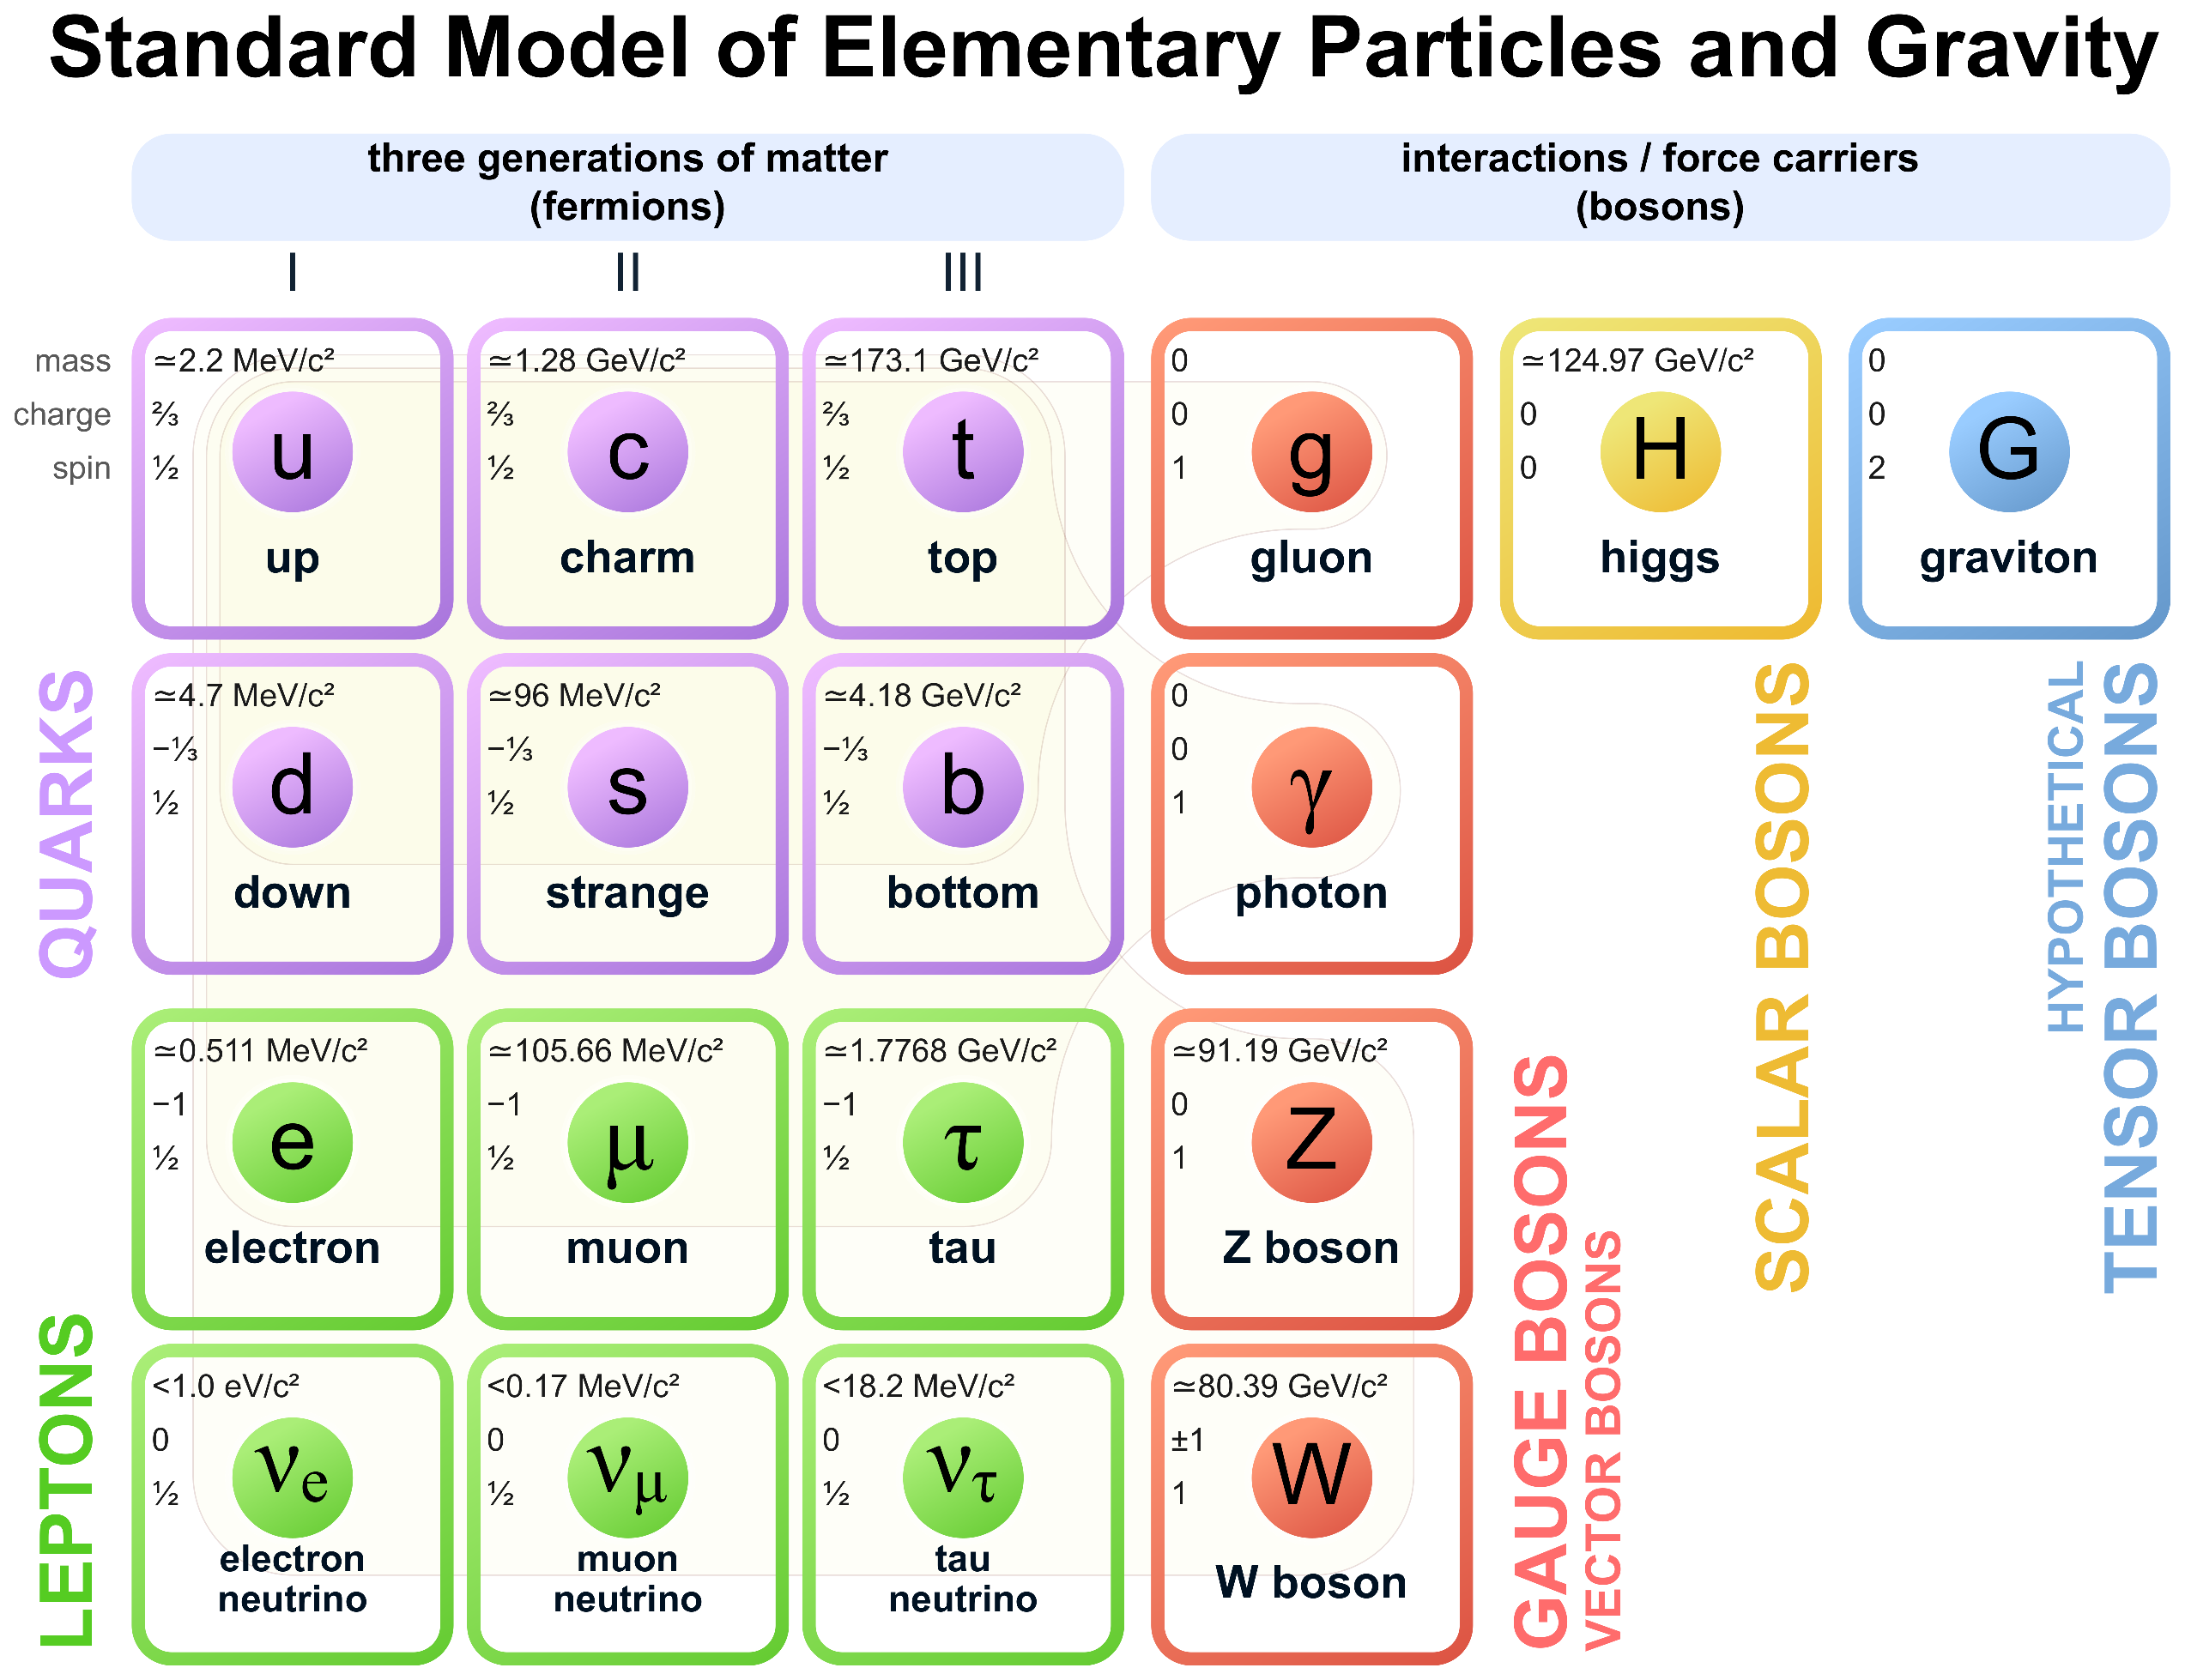
\includegraphics[scale=0.34]{MainContent/Figs/SM.eps}
	\caption{Standard Model. Fundamental particles are divided into Fermions and Bosons (force carriers). Fermions are divided into Quarks and Leptons and also in three differente generations. This figure was retrieved from}
	\label{fig:sm}
\end{figure}

\section{QCD}
\section{$B^0_s$}
\subsection{$B^0_s \to J/\psi\phi$}


% Chapter 2
\chapter{\leavevmode\newline The Large Hadron Collider}
\label{chap:chapter_2}

The Large Hadron Collider (LHC) is the largest particle collider in the world. It is located inside a 26.7 km long underground tunnel in the facilities of the European Organization for Nuclear Research (CERN), near Ginebra. This tunnel was used in the past for the Large Positron-Electron Collider (LEP) before it was shut down in 2000 \cite{stiller2016full, baron2018desarrollo}.

The LHC's initial goal was to detect the Higgs Boson. In order to accomplish this, it began operations in 2008, but due to a major incident known as "quench," it was shut down until the end of 2009 \cite{di2020measurement, oneill_2015}. The Higgs boson was finally detected in 2012 by CERN researchers \cite{cern_document_server_2012}. On top of that, many other predictions of the SM have been confirmed using the LHC experimental infrastructure, and it has also been possible to study the phenomena the SM cannot explain, as described in the previous chapter.
%https://www.universetoday.com/21895/first-images-emerge-of-damage-to-the-lhc/

To generate collisions in the LHC, two beams of target particles are generated using the Proton Synchrotron (PS) and the Super Proton Synchrotron (SPS), and then they are accelerated in opposite directions at energies of up to 460 GeV \cite{grummer2021search, bragagnolo2021measurement, mejia2012medida}. The target particles can be proton-proton (pp), lead ions (Pb-Pb) or proton-lead (p-Pb). There are four points where collisions occur, and there is a detector associated with each point, as shown in Fig. \ref{fig:LHC}. Two of these detectors are for general purposes: A Toroidal LHC Apparatus (ATLAS) and Compact Muon Solenoid (CMS) \cite{baron2018desarrollo, bonanomi2021response}. The other two are the LHC beauty detector (LHCb) used to study heavy-flavor physics and indirect CP violations in b-mesons, and A Large Ion Collider Experiment (ALICE) used for heavy-ion collisions \cite{stiller2016full, bonanomi2021response}.

The results and analysis presented in later chapters are based on CMS. Therefore, a detailed description of this detector will be given in the section \ref{section:cms}

\begin{figure}[htp!]
	\centering
	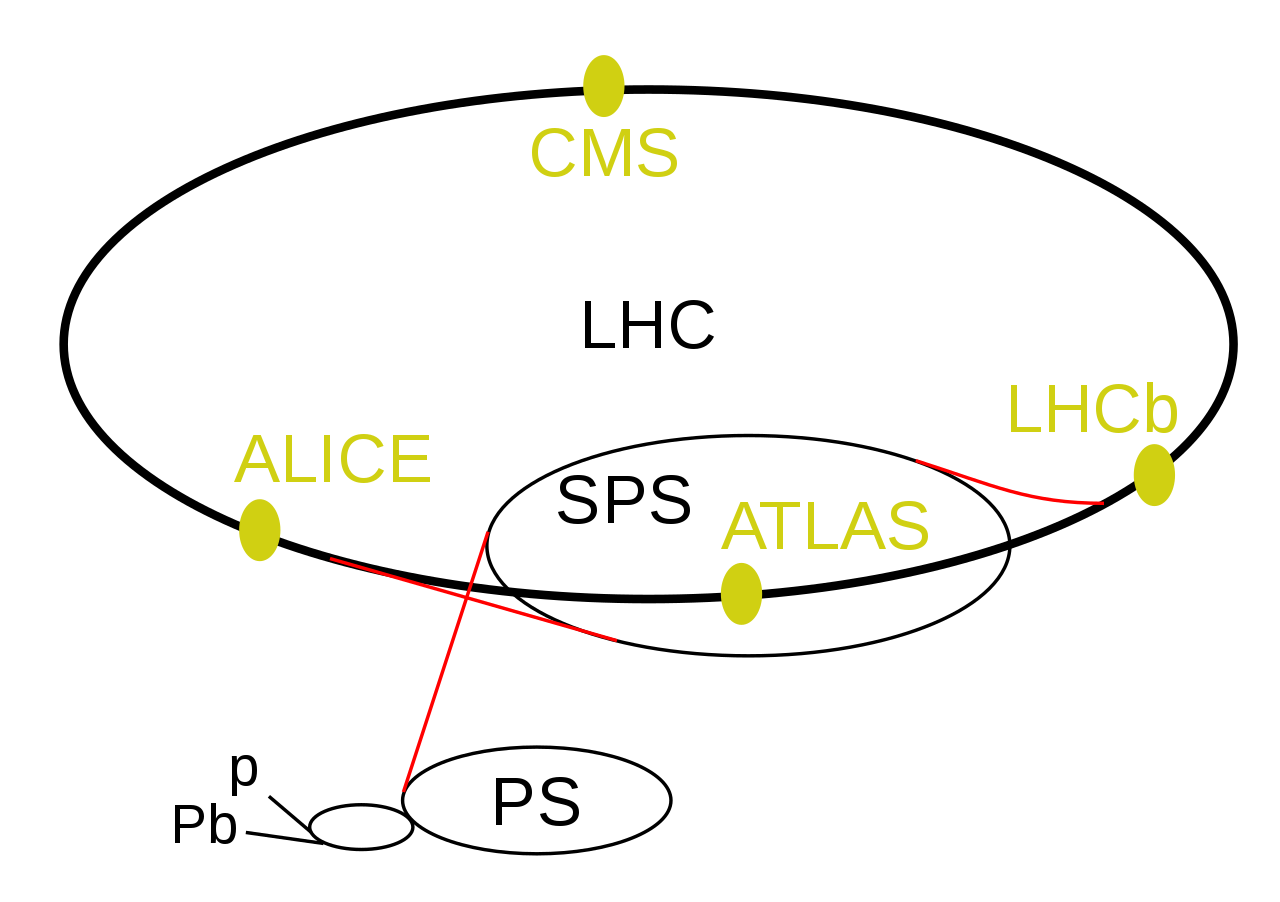
\includegraphics[scale=0.3]{MainContent/Figs/LHC.png}
	\caption{LHC experimental chain. The yellow dots represent the four main experiments. Retrieved from \cite{nobrega2013lhc}}
	\label{fig:LHC}
\end{figure}

\section{The CMS detector}
\label{section:cms}

CMS is a general purpose detector used to reconstruct the decay products in proton and heavy-ion collisions at high energies. It can detect nearly any particle, especially muons, with high precision. CMS is located in a cavern about 100 m underground near Cessy, France. It has a cylindrical geometry, with a full length of 21.5 m and a diameter of 15 m. With a total weight of 12500 t, it is the heaviest detector in the LHC \cite{bragagnolo2021measurement, mejia2012medida}. CMS is run by a large global collaboration of members, including over 4000 particle physicists, engineers, computer scientists, technicians, and students from over 200 institutes and universities in over 40 countries \cite{cms_collab}. Universidad de Antioquia is one of the collaborating universities through the Phenomenology and Fundamental Interactions Group (GFIF) \cite{restrepo2019udea}.

The physical structure of the detector consists of a superconducting solenoid able to produce an internal, uniform magnetic field of 4T. Inside the solenoid, there is a tracking system, also known as tracker, surrounded by a calorimetry system made up of the Electromagnetic Calorimeter (ECAL) and the Hadron Calorimeter (HCAL). Outside the solenoid, there is a muon detector chamber. The detector is depicted schematically in Fig. \ref{fig:CMS_structure}.

\begin{figure}[htp!]
	\centering
	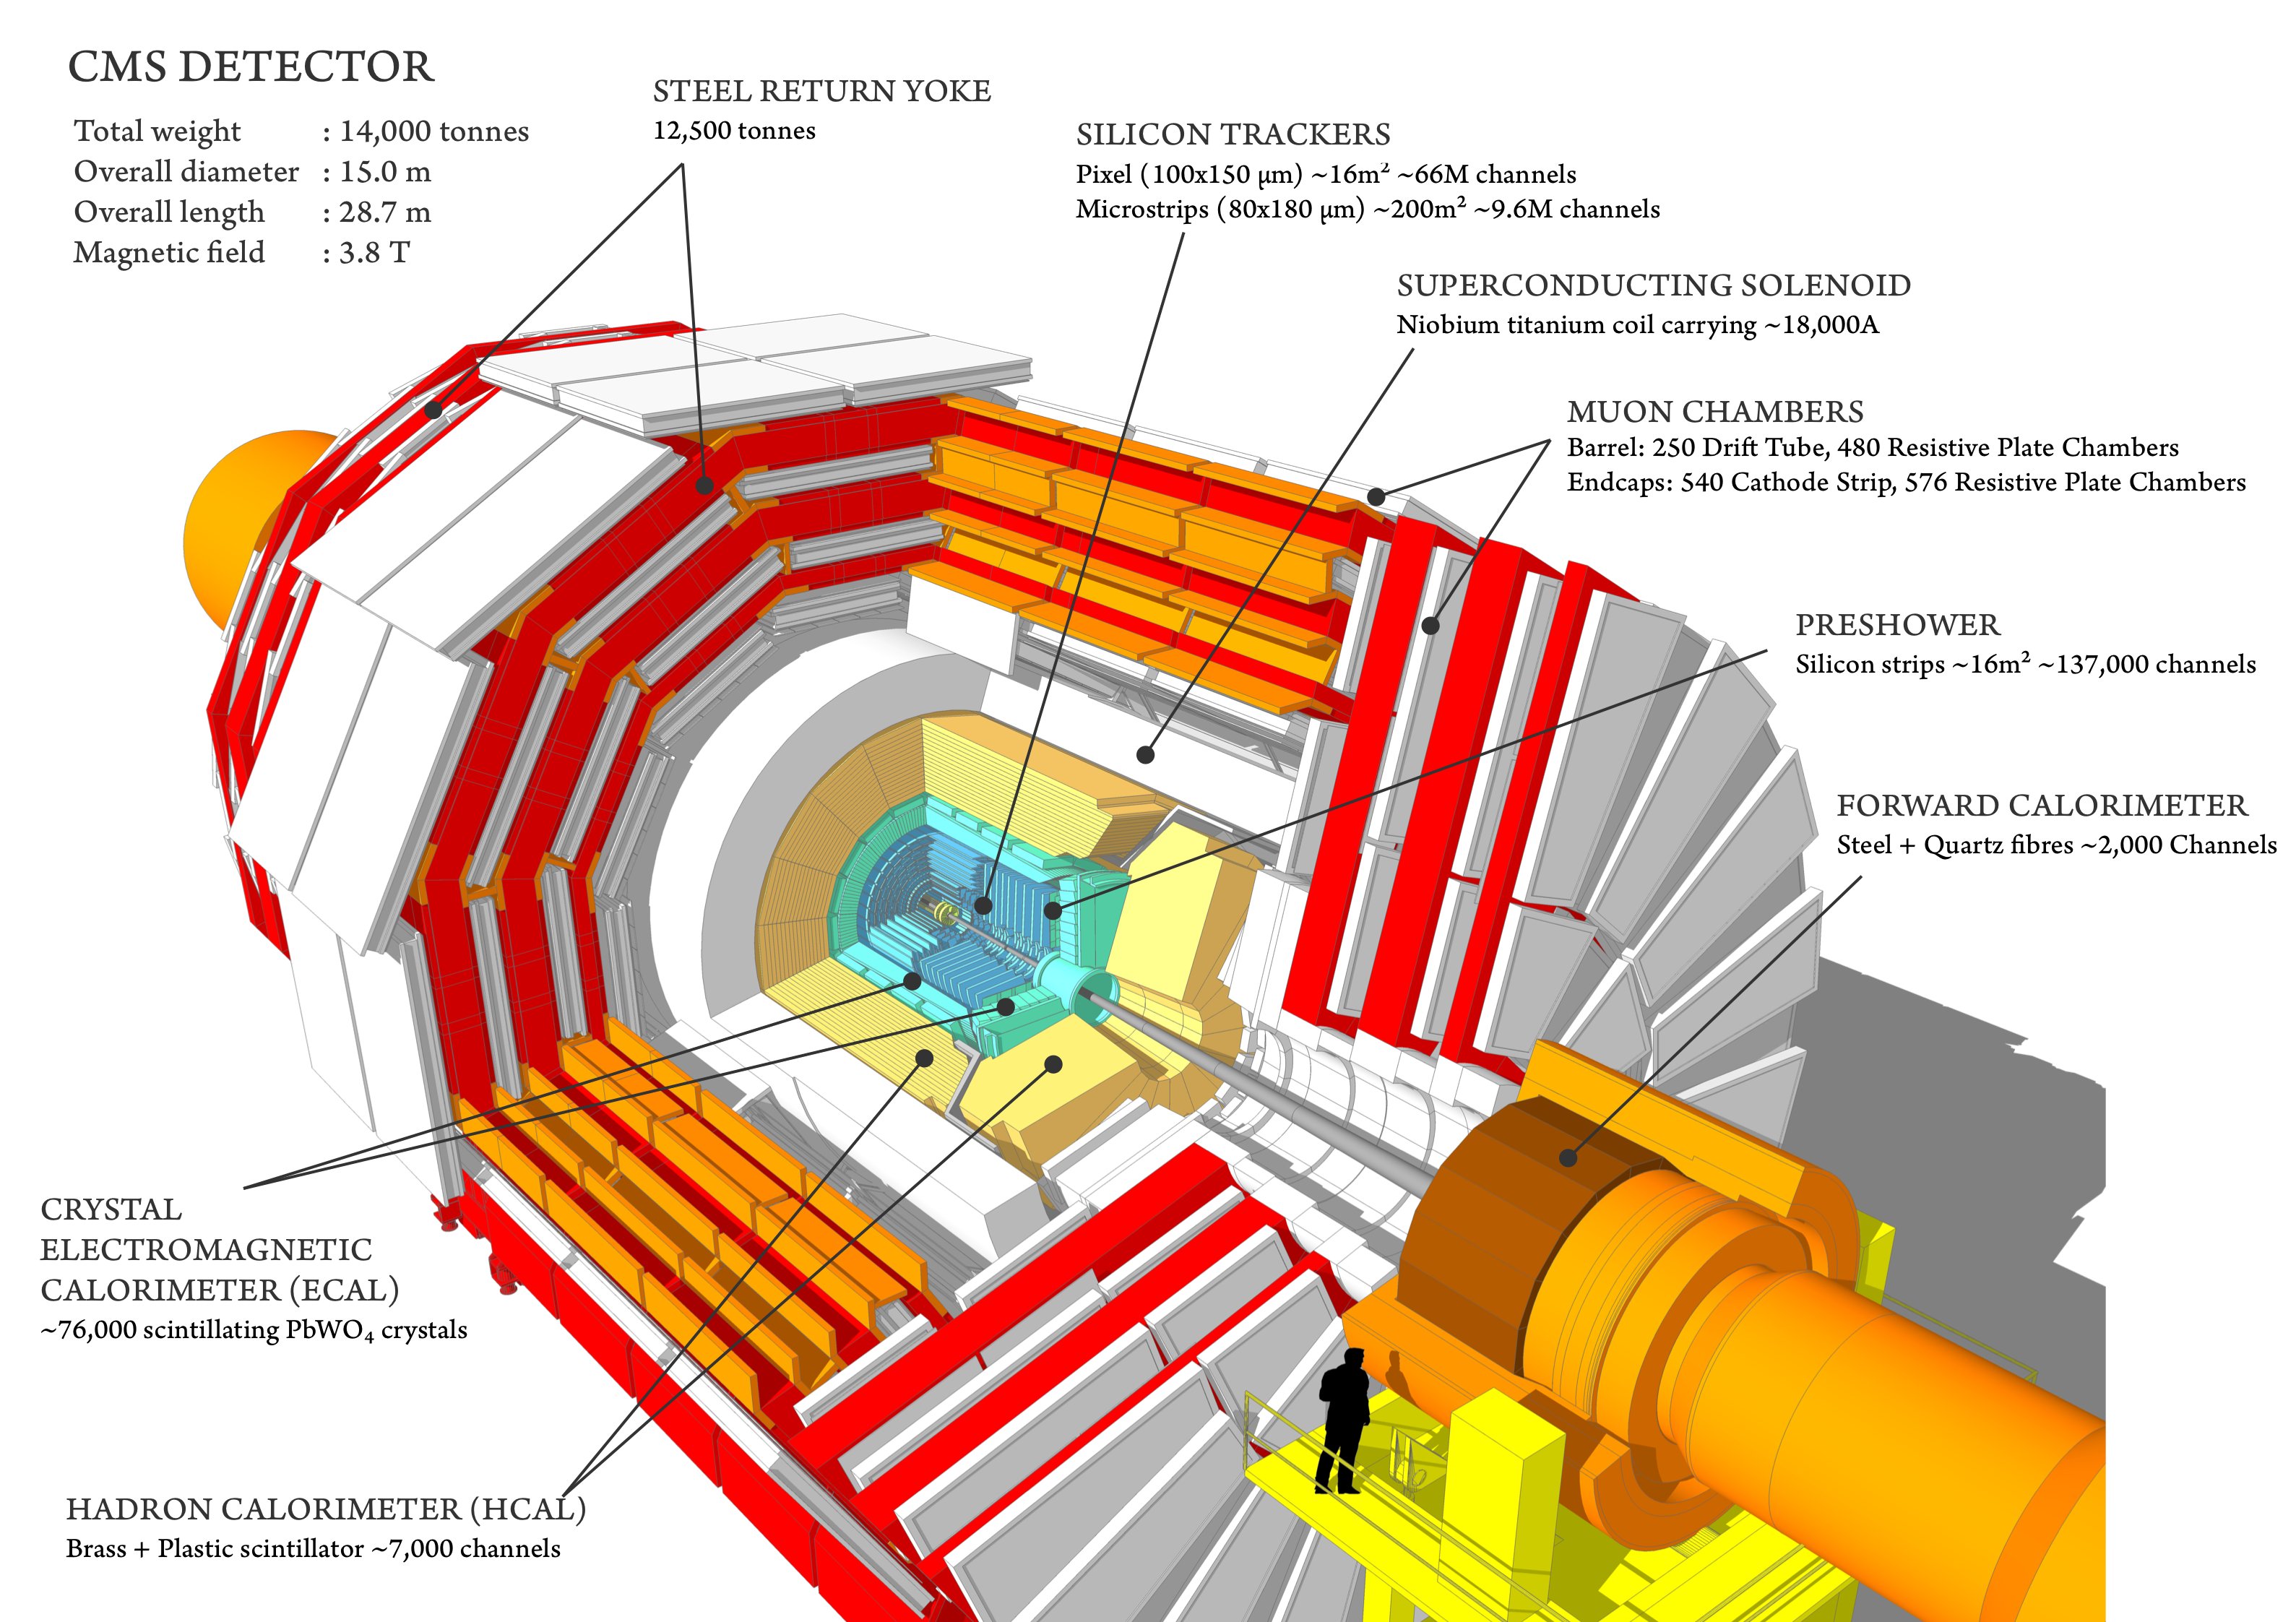
\includegraphics[scale=0.2]{MainContent/Figs/cms_structure.png}
	\caption{CMS internal structure with its main sub-systems. Retrieved from \cite{sanchez2020search}.}
	\label{fig:CMS_structure}
\end{figure}


Before delving deeper into the detector internal components, the coordinate system will be introduced in the following subsection.

\subsection{The coordinate system}
CMS uses a right-handed Cartesian coordinate system, with the origin at the center of the detector. The $x$-axis points towards the center of LHC, the $y$-axis points upwards, and the $z$-axis points in the counterclockwise direction of the beam. The $x-y$ plane is called the transverse plane and is perpendicular to the beam axis \cite{baron2018desarrollo, sanchez2020search, lechner2021measurement}. In this plane, two quantities can be defined: the azimuthal angle $\phi$ with respect to the x-axis and the particle transverse momentum, $p_T = \sqrt{p_x^2 + p_y^2}$. The polar angle $\theta$, on the other hand, is defined in the $z-y$ plane and measured from the $z$-axis. Fig. \ref{fig:cms_coordinate_system} illustrates the coordinate system.


\begin{figure}[htp!]
	\centering
	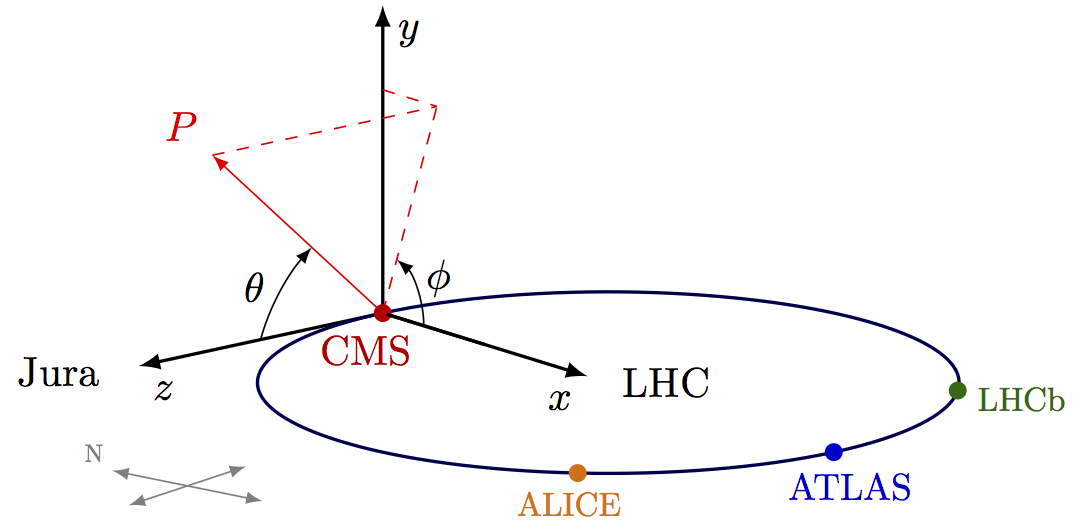
\includegraphics{MainContent/Figs/cms_coordinate_system.png}
	\caption{Illustration of the CMS coordinate system. Retrieved from \cite{bonanomi2021response}.}
	\label{fig:cms_coordinate_system}
\end{figure}

In this coordinate system, one can define two relativistic invariant quantities, the particle rapidity \cite{bonanomi2021response},

\begin{equation}
y = \frac{1}{2}\ln\left(\frac{E+p_z}{E-p_z}\right)
\end{equation}

and the pseudo-rapidity,

\begin{equation}
\eta = -\frac{1}{2}\ln\left(\frac{\theta}{2}\right)
\end{equation}

It is important to mention that the quantities $p_T$, $\eta$ and $y$ are considered in the reconstruction presented in \ref{chap:Chapter_3}, and the results from chapter \ref{chap:Chapter_4} and \ref{chap:Chapter_5}.
\subsection{Superconducting Solenoid}
Located at its center, the superconducting solenoid is the key part of the CMS detector. The solenoid is made up of four layers of Nb-Ti coils, has a length of 12.5 m and a diameter of 6 m. It works at a temperature of 4.5K and it can produce a constant magnetic field inside of 4T, however, it is normally operated at 3.8T \cite{baron2018desarrollo, bragagnolo2021measurement}. A return yoke made of iron reduces the magnetic field outside the solenoid to about 2T. The magnet stores a total energy of 2.6 GJ \cite{fedi2016studies}. The magnetic field is used to bend the trajectory of the charged particles after the collision, thus allowing to measure their transversal momentum, $p_T$, and charge sign. The stronger the magnetic field, the larger the bending, and, hence, more precise measurements can be achieved \cite{sanchez2020search, presilla2021lepton}.
\subsection{The tracker}
The tracker, which is placed at the interaction point, is made up of two parts: a silicon pixel detector in the center and a silicon strip detector around it, both of which are made of superconducting technology but have different sizes and granularities \cite{sanchez2020search}. The pixel detector is very granular and consists of 66 million pixels spaced out over a radius of 10 cm, each pixel has a dimension of $100 \times 150 \ \mu \text{m}^2$. The strip detector contains 9.6 million of strips and has a length of 5.5 m and a diameter of 2.4 m \cite{fedi2016studies, danilov2020measurement}.

An electron-hole pair is formed in the material when a charged particle passes through the tracker. This generates an electrical signal, which is amplified and used to reconstruct the trajectory or tracks with a 98$\%$ percent efficiency and a precision of about $10 \ \mu$m in the range $|\eta| < 2.5$ \cite{baron2018desarrollo, di2020measurement}. The momentum of a particle is calculated using the trajectory. The tracker can also estimate the location of the secondary vertices where decays occur \cite{fedi2016studies}.
\subsection{Calorimetry system}
\label{cal_sys}
The calorimetry system of CMS is placed after the tracker. The reason for this is that the calorimetry system measures the energy of most particles by fully absorbing them, with the exception of neutrinos and neutrons \cite{bragagnolo2021measurement}. To achieve high accuracy in measurements, the system is divided into two sub-detectors, the ECAL and the HCAL, which are located between the tracker and the superconducting solenoid, with the ECAL in the innermost part \cite{presilla2021lepton}.

ECAL is a cylindrical detector that measures electron and photon energies and covers the pseudo-rapidity, $|\eta| < 3$. The ECAL is made up of approximately 76000 scintillating crystals of lead tungstate (PbWO$_4$) \cite{fedi2016studies, mejia2012medida}. This material was chosen because of its high density, short radiation length, and small Moliere radius \cite{danilov2020measurement}. It is also highly transparent due to its low concentration of oxygen, this is particularly useful because when photons and electrons pass close by, it scintillates with a light with an intensity proportional to the particle's energy. Photodetectors are used to measure this light \cite{di2020measurement, mejia2012medida}.

HCAL is a sampling and hermetic calorimeter with brass layers and plastic scintillators. It measures the energy of charged and neutral hadrons (protons, pions, kaons, neutrons, and so on) in the region $|\eta| < 5$ \cite{li2021measurements, muhammad2021measurement}. To accomplish this, when a particle passes close by, the brass layers produce a secondary hadron shower, and when these secondary hadrons interact with the scintillators, light is produced, which is then converted into an electric signal by hybrid photodiodes \cite{baron2018desarrollo, muhammad2021measurement}. HCAL can also measure the missing energy in the transverse plane, $E^{\text{miss}}_T$, which is primarily associated with weakly interacting particles such as neutrinos \cite{di2020measurement}.
\subsection{Muon detector}
CMS's name derives from one of its primary goals: muon detection. Muons are not absorbed by the calorimetry system due to their high penetrative power \cite{baron2018desarrollo, di2020measurement}. As a result, a system of muon detectors is installed in the CMS's outermost region. This system not only detects muons with high efficiency in the $\eta < 2.4$ region, but also measures their momenta, charge, and triggers when they are present \cite{sanchez2020search}. The muon detection method is based on gaseous technology: a charged particle ionizes a gas, causing drift currents that are later read out \cite{baron2018desarrollo, danilov2020measurement}.

The system is composed of three gaseous chambers: Drift Tubes (DT), Chatode Strip Chambers (CSC), and Resistive Plate Chambers (RPC). There are a total of 250 DTs located in the barrel region, covering $|\eta| < 1.2$. This has a nearly uniform magnetic field and low rate of particles. DTs can provide measurements in the $r\phi$ plane and the $z$-direction \cite{bragagnolo2021measurement, di2020measurement, muhammad2021measurement}. CSCs, on the other hand, are found in the endcap where there is a strong and non-uniform magnetic field. They cover the pseudorapidity $0.9 < |\eta| < 1.2$ and provide measurements of the hit coordinates. There are four layers, each with 540 CSCs chambers \cite{lechner2021measurement, muhammad2021measurement}. Finally, the triggering is carried out using approximately 1056 RPCs modules. They have a high time resolution of about 1 ns. Each module is made up of two parallel plates separated by a gas and operated in avalanche mode. RPCs are placed in both the barrel and endcaps and cover the region $|\eta| < 1.9$ \cite{di2020measurement, lechner2021measurement}.

At the time of writing this manuscript, 144 new muon detectors known as Gas Electron Multipliers (GEMs) had been installed in the CMS detector. Their main goal is to improve muon track identification and enable wider measurements in the forward region (the endcaps), where high doses of radiation are present. It is expected that 288 additional GEMs will be installed between 2023 and 2024 and 216 during between 2025 and 2027 \cite{cern2020ls2, cerngems}. Universidad de Antioquia is a member of the GEMs team, primarily assisting with hardware tests and software development \cite{cms25udea}. GEMs are not significant for this dissertation because the data used for analysis was collected in 2016.

\subsection{Trigger System}
\label{subsection:trig_sys}
In a single second, the amount of data derived from collision events is approximately $1$ PB (Petabyte) \cite{baron2018desarrollo}. With today's technology, it is impossible to save all the data generated during an experiment and not all of this data is actually relevant to the CMS program. As a result, a trigger system is used to reduce the amount of data that must be processed. The filtering process in the trigger is divided into two stages \cite{muhammad2021measurement}. The data is first passed through a hardware-based filter known as the Level-1 (L1) trigger, and then it is passed through the High-Level Trigger (HLT).

The L1 trigger must decide whether an event is to be disregarded in a short time interval of about 4 $\mu$s \cite{bragagnolo2021measurement}. To do so, it takes the input from the sub-detectors in the calorimetry and muon system and processes it with hardware-based algorithms that run in parallel on several FPGAs and ASICs \cite{muhammad2021measurement}. This information is roughly processed and reconstructed into simple physics objects such as muons, photons, electrons, jets, and their associated transverse energy. An algorithm called \verb|Global Trigger| decides if the event is passed to the HLT trigger. The L1 trigger reduces the rate of event generation to around 100 KHz \cite{bragagnolo2021measurement, muhammad2021measurement}.

The HLT trigger uses a set of software-based algorithms that run in a farm of processors made up of commercial CPUs to process the events filtered by the L1 trigger \cite{bragagnolo2021measurement}. These algorithms are pre-selected based on the object of study. HLT uses data from all the detectors in the CMS to partially reconstruct the entire event \cite{bragagnolo2021measurement}. The decision time is approximately 200 ms, and HLT is capable of reducing the event production rate from 100KHz to approximately 200 Hz. This data can then be saved for offline use \cite{fedi2016studies, danilov2020measurement}.

% Chapter 3
\chapter[\leavevmode\newline Simulation and $B^0_s$ Reconstruction]{Simulation and $B^0_s$ Reconstruction}
\chaptermark{Simulation and $B^0_s$ Reconstruction}
\label{chap:Chapter_3}
\section{Data and Monte Carlo samples}
The official dataset used for analysis was the \verb|/PADoubleMuon/PARun2016C-PromptReco-v1/AO| dataset and it was collected with the CMS experiment during the 2016 proton-nucleus (p-Pb) collisions at $\sqrt{s_{NN}} = 8.16$ TeV, with a total integrated luminosity of 179.7 nb$^{-1}$. Monte Carlo (MC) samples are generated prior to using this dataset. These samples can be used to estimate the detector efficiency, the performance of measurement methods described in Chapter 4, and choosing the parameters for reconstruction  of the $B^0_s \to J/\psi \ \phi(1020)$ channel with the real dataset. In order to generate the MC examples, the general-purpose generator \verb|PYTHIA 8| is used to simulate the particle production and hadronization process. The decay of the b hadrons is modeled with the \verb|EVTGEN| package. The \verb|EVTGEN| module \verb|PHOTOS| calculates the final state radiation (FSR). Lastly, the response of the CMS detector is simulated by the software \verb|GEANT4|. This software is set up with the same triggers and reconstruction algorithms used for the dataset of the collision. %The total number MC samples generated was 

\section{Triggers}
As explained in \ref{subsection:trig_sys} a trigger needs to be implemented in order to select the events of real interest. For the current work, a high level filter labeled as \verb|HLT_PAL1DoubleMuOpen_v1| is used. This is a rather loose trigger that softens the preselection criteria of the two muon candidates to maximize detection efficiency. It should be noted that a trigger prescale is sometimes used, this refers to the selection of only one event from a set of events that bypass the trigger requirements while disregarding the rest \cite{dorigo_2014}. However, no prescaling was used during the 2016 p-Pb collisions, resulting in a higher statistical precision.

\section{Reconstruction and selection criteria}%triggers
To reconstruct the $B^0_s$ meson via the chosen channel, the $J/\psi$ and $\phi (1020)$ mesons must first be reconstructed. For the $J/\psi$ meson, two muon candidates are required, and two kaons are required for the $\phi (1020)$ meson. The specific selection criteria for such candidates will be described in the following sub-sections.
\subsection{J/$\psi$ reconstruction}

Only pairs of muons with opposite charge sign are considered ($\mu^{+}\mu^{-}$). Both muons are required to classify as Soft Muons. They must originate from a common vertex, with a  $\chi^2$ vertex probability, $J_{pro} > 1\%$. It is also necessary for both muons to have $|\eta| < 2.4$ and the following $p_T$:

\[ \begin{cases} 
	p_T > 3.3 \ \text{GeV} & |\eta| < 1.1 \\
	p_T > \left(5.5 - 2.0 \times |\eta|\right) \ \text{GeV} & 1.1 \leq |\eta| < 2.1 \\
	p_T > 1.5 \ \text{GeV} & 2.1 \leq |\eta| < 2.4 
\end{cases}
\] 

As a final condition for selecting a muon pair, the dimuon invariant mass must be in the range $[2.9, 3.3]$ GeV.
\subsection{$\phi(1020)$ reconstruction}
After selecting the appropriate muon candidate tracks, and because the CMS detector cannot correctly identify the tracks, it is assumed that the remaining tracks are kaon tracks, and thus all of them are initially considered for the $\phi(1020)$ reconstruction. However, in order for two pairs of kaons to be valid candidates, they must have opposite charge ($K^{+}K^{-}$), $|\eta| < 2.4$ and $p_T > 0.8$ GeV and have high purity. The invariant mass of the kaon-pair must be between $0.010$ GeV around the reported mass for $\phi(1020)$ in the PDG of $1.01946$ GeV.
\subsection{$B_s^0$ reconstruction}
Once the $J/\psi$ and $\phi(1020)$ candidates are properly reconstructed, they are required to have a common vertex, which corresponds to the $B_s^0$ vertex. The invariant mass of the $J/\psi$ - $\phi$ pair must be in the range $[5.240, 5.490]$ GeV, also the $p_T$ for the $B_0^s$ candidate must be in the range $[7, 50]$ GeV. 

Several variables are used to reconstruct the $B_0^s$ meson, and due to the presence of high combinational background, it is desirable to find the optimal parameters for these variables that maximize the statistical significance of the signal:

\begin{equation}
	S = \frac{N_{\text{signal}}}{\sqrt{N_{\text{signal}} + N_{\text{bkg}}}}
\end{equation}

This optimization was performed using the MC samples. The variables used and their corresponding optimal value were: decay-length significance, $c\tau / \sigma_{c\tau}< 6.0 $, one of the kaons $p_T > 0.9$ and a $\chi^2$ vertex probability $B_{pro} > 3 \%$.

A summary of the selection criteria for the reconstruction of the three objects is presented in table \ref{table:sel_criteria}.
\begin{section}{CMSSW Framework}
The simulation and event reconstruction described above were all carried out using \verb|CMSSW|, a \verb|C++|-based framework provided by CMS. \verb|Python| is widely used as well. \verb|CMSSW| was designed to make it easier to analyze and process data from detectors \cite{di2020measurement, twiki2013}. To do so, it employs an event data model, in which for each event that passes the trigger selection, a \verb|C++| class known as \verb|Event| is generated \cite{fedi2016studies, muhammad2021measurement}. This class contains all the necessary information about the event. After processing the data with  \verb|CMSSW|, a structured and user-friendly file format known as  \verb|ROOT| is generated, which can then be used for analysis by physicists, such as the one described in the following chapter \cite{di2020measurement}.
\end{section}
\setlength{\tabcolsep}{0.5em} % for the horizontal padding
{\renewcommand{\arraystretch}{1.4}% for the vertical padding
	\begin{table}[!htp]
		\label{table:sel_criteria}
		\begin{center}
		\begin{tabular}{cc}
			\hline                                                         \multirow{2}{*}{\textbf{Reconstruction}}    & \multirow{2}{*}{\textbf{Selection Criteria}}                                                                                                                                                                            \\
			&                                                                                                                                                                                                                         \\ \hline
			\multirow{5}{*}{$J/\psi \to \mu^{+}\mu{-}$} & Soft-Muon                                                                                                                                                                                                               \\ \cline{2-2} 
			& $|\eta|_{\mu_i} < 2.4$                                                                                                                                                                                                          \\ \cline{2-2} 
			& \begin{tabular}[c]{@{}c@{}}$(p_T)_{\mu_i} > 3.3 \text{GeV if } |\eta|_{\mu_i} < 1.1$\\ $(p_T)_{\mu_i} > \left(5.5 - 2.0 \times |\eta|_{\mu_i}\right) \text{GeV if }  1.1 \leq |\eta|_{\mu_i} < 2.1$\\ $(p_T)_{\mu_i} > 1.5 \text{GeV if } 2.1 \leq |\eta|_{\mu_i} < 2.4$\end{tabular} \\ \cline{2-2} 
			& $M(\mu^{+}\mu^{-}) \in [2.9, 3.3] GeV$                                                                                                                                                                                  \\ \cline{2-2} 
			& $\chi^2$ vertex probability $ > 1 \%$                                                                                                                                                                                   \\ \hline
			\multirow{4}{*}{$\phi(1020) \to K^{+}K{-}$} & High-Purity Track                                                                                                                                                                                                       \\ \cline{2-2} 
			& $|\eta|_{K_i} < 2.4$                                                                                                                                                                                                          \\ \cline{2-2} 
			& $(p_T)_{K_i} > 0.8$ GeV                                                                                                                                                                                                         \\ \cline{2-2} 
			& $|M(K^{+}K^{-}) - M_{PDG}(\phi)| <  0.010$ GeV                                                                                                                                                                          \\ \hline
			\multirow{4}{*}{$B^0_s \to J/\psi \phi$}    & $p_T \in [7.0, 50.0]$ GeV                                                                                                                                                                                               \\ \cline{2-2} 
			& $M(J/\psi \phi) \in [5.240, 5.490] $ GeV                                                                                                                                                                                \\ \cline{2-2} 
			& $c\tau / \sigma_{c\tau}< 6.0 $                                                                                                                                                                                          \\ \cline{2-2} 
			& $\chi^2$ vertex probability $ > 3 \%$                                                                                                                                                                         \\ \hline
		\end{tabular}
		\caption{Criteria for the selection and reconstruction of the $B^0_s \to J/\psi \phi$ decay using the $J/\psi \phi \to \mu{+}\mu{-}$ and $\phi(1020) \to K^{+}K^{-}$ decays.}
		\end{center}
	\end{table}

% Chapter 4
\chapter[\leavevmode\newline Analysis Methods]{Analysis Methods}
\chaptermark{Analysis Methods}
\label{chap:Chapter_4}

The experiments performed in CMS are of random nature. This refers to an experiment in which the output cannot be precisely predicted given a set of known inputs and initial conditions. Moreover, with each try, a different value may be obtained even if the inputs and conditions are the same. As a result, the various outputs or outcomes must be statistically treated in order to estimate the probability of getting a given output \cite{vsirca2016probability}. This chapter will explain the statistical methods used for analysis in the current thesis.
\section{Probability Density Function}

Given a continuous random variable $X$, a probability density function (PDF) $f_X$ is a mathematical function that describes the probability that $X$ has a value in the range $[a, b]$ \cite{bragagnolo2021measurement, vsirca2016probability}:

\begin{equation}
	\int_{a}^{b} f_X(x) \ dx = P(a < X < b)
\end{equation}

with the properties that it is normalized, $\int_{-\infty}^{\infty} f_X(x) \ dx = 1$ and it is non-negative, $f_X(x) \geq 0$.

If the invariant mass of the $B^0_s$ is regarded as a random variable, then a PDF can be used to model its distribution or spectra. Since this mass spectra is the primary focus of this manuscript, a detailed description of the chosen PDF will be provided in the following section.
\section{PDF for the invariant mass of $B^0_s$}
The data associated to the mass distribution can be classified as either signal or background data. The signal data are events that truly correspond to the $B^0_s$ decaying in the desired channel, whereas the background data can be either partially reconstructed $B^0_s$ mesons or events that, while meeting selection criteria, do not correspond to this meson \cite{mejia2012medida}.

The signal data is modeled using a PDF consisting of the sum of two gaussian distributions with the same mean value but different standard deviations:

\begin{equation}
S_{PDF}(M_i) = \frac{1}{\sqrt{2\pi}} \left(f_s \cdot \frac{1}{\sigma_1}e^{-\frac{1}{2}\left(\frac{M_i-\mu}{\sigma_1}\right)^2} + (1 - f_s) \cdot \frac{1}{\sigma_2}e^{-\frac{1}{2}\left(\frac{M_i-\mu}{\sigma_2}\right)^2}\right)
\end{equation}

Where $M_i$ is the value of the invariant mass, $\mu$ is the mean value and $\sigma_1, \sigma_2$ are the standard deviations of each gaussian. $f_s$ is the fraction of $S_{PDF}$ that corresponds to the first gaussian and $1-f_s$ to the second gaussian. 

The PDF used to model the background data corresponds to an exponential function:

\begin{equation}
B_{PDF}(M_i) = A \cdot e^{-cM_i}
\end{equation}

With $A$ the normalization constant. 

Finally, the PDF for the mass is obtained by adding both PDFs:

\begin{equation}
M_{PDF}(M_i) = N_s \cdot S_{PDF}(M_i)  + N_b \cdot B_{PDF}(M_i)
\label{eq:masspdf}
\end{equation}

Where $N_s$ and $N_b$ refer to the number of signal and background events respectively. This PDF is used for both the collision and MC data.

\section{Maximum likelihood method}
\label{mlmethod}
The parameters used to define the PDF of a random variable $X$ are usually unknown. If the value of $X$ is measured several times, the values of the unknown parameters can be determined using the maximum likelihood (ML) method, as described below.

Let $f_X(\vec{x}, \vec{\Theta} )$ be a PDF described by $N$ measured values of $X$, $\vec{x} = \{x_1, x_2, ..., x_N\}$, and $M$ unknown parameters, $\vec{\Theta} = \{\Theta_1, \Theta_2, ..., \Theta_M \}$, then the likelihood function is defined as the product of the values of the PDF for each observation \cite{bonanomi2021response,vsirca2016probability}:

\begin{equation}
L(\vec{x} \ | \ \vec{\Theta}) = \prod_{i = 1}^{N} f_X(x_i, \vec{\Theta}) 
\end{equation}

Where $|$ denotes the fact that this is a joint probability. The ML method consists of estimating the optimal values for the parameters $\Theta$ by maximizing the logarithm of the likelihood function \cite{mejia2012medida},

\begin{equation}
	l(\vec{x} \ | \ \vec{\Theta}) = \log L(\vec{x} \ | \ \vec{\Theta}) = \sum_{i = 1}^{N} \log f_X(x_i, \vec{\Theta})
\end{equation} 

with respect to $\Theta$:

\begin{equation}
	\frac{\partial{l(\vec{x} \ | \ \vec{\Theta})}}{\partial \Theta_j} = \sum_{i = 1}^{N} \frac{1}{f_X(\vec{x}, \vec{\Theta})} \frac{\partial{f_X(\vec{x}, \vec{\Theta})}}{\partial \Theta_j} = 0
\end{equation} 

\begin{equation}
	\frac{\partial^2{l(\vec{x} \ | \ \vec{\Theta})}}{\partial \Theta_j ^2} < 0
	\label{eq:ml}
\end{equation}

with $ j = 1, 2, ..., M$. The optimal value for the unknown parameter, $\Theta_j$, can be obtained by solving the respective differential equation.

There is a extended version of the ML method, used when the number of of measured values $N$ is also an unknown parameter. In this version, it is assumed that $N$ follows a Poisson distribution, therefore, the likelihood function changes to \cite{bonanomi2021response}:

\begin{equation}
	L(\vec{x} \ | \ \vec{\Theta}, \nu) = \frac{e^{-\nu} \nu^N}{N!} L(\vec{x} \ | \ \vec{\Theta})
\end{equation}

where $\nu$ is the expected number of observations. 
If $\nu$ does not depend of $\Theta$, then $\nu = N$. 

Typically, no analytical solution exists for this maximization problem, necessitating the use of numerical methods. As a result, an algorithm in \verb|C++| is written in which the library \verb|ROOTFIT| is used to perform the ML method in the extended version. This version was chosen because the number of signal and background events, $N_s$ and $N_b$, are of interest and their values are unknown in advance.

The fit is done initially on the MC data, with all parameters set free. Then, when using the real dataset, the parameters $\sigma_1, \ \sigma_2$, and $f_s$ in the signal PDF are fixed to the values obtained with the MC data. The complexity of the fit is considerably decreased in this manner since there are less parameters to be determined by the ML extended method. The background PDF, on the other hand, has no alteration. The real data of the invariant mass is fitted and the values for the number of signal and background events, $N_s$ and $N_b$ are obtained. 

\section{Significance}
\label{sec:sig}
Because of the high combinational background, it's important to find a set of additional conditions in the selection of the $B^0_s$ candidates, among the many that may be established, that reduces the number of background events while increasing the number of signal events. This can be accomplished by maximizing the signal's statistical significance, which is defined as:

\begin{equation}
	\label{eq:sig}
	S = \frac{N_{\text{s}}}{\sqrt{N_{\text{s}} + N_{\text{b}}}}
\end{equation}

With respect to a set of parameters. The parameters used in this case were the decay-length significance, $c\tau / \sigma_{c\tau}$, $p_T$ of kaons and $\chi^2$ vertex probability of $B^0_s$, $B_{pro}$ and the following conditions where imposed:

\begin{itemize}
	\item  $(p_T)_{K_i} > a$, with $a \in [0.5, 1.2]$ GeV.
	\item $B_{pro} > b$ with $b \in [1, 10] \%$ 
	\item $c\tau / \sigma_{c\tau} < c$ with $c \in [1, 7]$
\end{itemize}

$a$, $b$, and $c$ are the values for which $S$ is maximum, and they were calculated by combining various alternative values for $a$, $b$, and $c$. A fit of the invariant mass is done for each combination, and $S$ is determined. The different values are compared, and $max(S)$ is found.
\section{Systematic and statistical uncertainties}
The uncertainties in the measurement of a quantity during a physics experiment can be classified by two types. The first type are the statistical uncertainties, which are related to the fact, as mentioned in the introduction of this chapter, that multiple measurements of the same quantity can yield different results. Therefore, the value of such quantity is not precise, but fluctuates within a range. The measurement of this range is the statistical uncertainty \cite{sinervo2003definition}. The statistical uncertainties are calculated by \verb|ROOTFIT|, and in the case of the ML method, these are determined by the covariance matrix $\mathrm{var}[\vec{\Theta}]$ \cite{vsirca2016probability}:

\begin{equation}
	\mathrm{var}[\vec{\Theta}] = 
	\left(-E\left[ \frac{\partial^2 l(x | \vec{\Theta}) }{\partial \vec{\Theta} ^2}\right]_{\Theta = \hat{\Theta}}\right)^{-1}
\end{equation}

with $E[X]$ the expected value of $X$. The diagonals are the variance of the parameters $\vec{\Theta}$ and the uncertainty is the square root of the variance, 

\begin{equation}
	\delta \Theta_i = \sqrt{\mathrm{var}[\Theta_i]}
\end{equation}

On the other hand, given a set of $N$ random variables $\vec{X}$ and a respective covariance matrix $\mathrm{var}[\vec{X}]$, if a function $f = f(\vec{X})$ depends on these variables, then the variance associated to $f$ is calculated by \cite{vsirca2016probability}:

\begin{equation}
	\mathrm{var}[f(\vec{X})] = \sum_{i=1}^N \sum_{j=1}^N \left(\frac{\partial f}{\partial X_i} \frac{\partial f}{\partial X_j} \right)_{X = \mu} \mathrm{var}[\vec{X}]_{i,j}
\end{equation}

with the partial derivatives evaluated at the mean value of $X$, $\mu$. When there is no correlation between variables, the previous equation reduces to:

\begin{equation}
	\label{totaluncertainty}
	\mathrm{var}[f(\vec{X})] = \sum_{i=1}^N  \left(\frac{\partial f}{\partial X_i}\right)^2_{X = \mu} \mathrm{var}[X_i]
\end{equation}

Revise \cite{vsirca2016probability} for more information on expected values, variance, and their relation to uncertainties. Alternatively, any statistical book on the subject would suffice.

The second type are systematic uncertainties. They are related to the nature of the instrument used, the specific model chosen for the data, the assumptions made about the experiment beforehand, among other factors. It should be noted that by taking more measurements of the quantity, the value of the statistical uncertainty can be minimized. For systematic uncertainties, however, this is not the case \cite{sinervo2003definition}. The uncertainties from different measurements are correlated, which means that they are not independent of one another. After a thorough examination and testing of the potential sources of uncertainty, systematic uncertainties can be calculated and possibly reduced. The total systematic uncertainty is calculated as:

\begin{equation}
	\delta_{sys} = \sqrt{\sum_{i}^{N} \delta_{{sys}_{i}}^2}
\end{equation}

where $\delta_{{sys}_i}$ represents each one of the individual systematic uncertainties.
%\begin{equation}
%	\delta_T = \sqrt{\delta_{stat}^2 + \delta_{sys}^2}
%\end{equation}

\section{$p_T$ and $|y|$ bins}

The influence of transverse momentum $p_T$ of the $B_0^s$ on the mass distribution is investigated. The dataset is partitioned into multiple regions or bins of $p_T$, to accomplish this. These bins have been chosen in order to provide helpful information on the statistics of the mass. The following boundaries determine the bins: $[7, 10, 15, 20, 50]$ GeV. In each of these regions, the mass spectrum is fitted. Similarly, the influence of rapidity $|y|$ of $B_0^s$ is investigated. And the boundaries for the bins were set at $[0, 0.5, 1, 1.6, 2.4]$ GeV.



% Chapter 5
\chapter[\leavevmode\newline Differential cross-section of $B^0_s \to J/\psi \phi$]{Differential cross-section of $B^0_s \to J/\psi \phi$}
\chaptermark{Differential cross-section of $B^0_s \to J/\psi \phi$}
\label{chap:Chapter_5}

\section{Total efficiency}

The acceptance $\alpha$ is defined as the ratio of the number of $B^0_s$ mesons that meet the filter criteria for the kaons and muons candidates to the total number of $B^0_s$ mesons created in the MC simulation,

\begin{equation}
\alpha(p_T, |y|) = \frac{N(B^0_s; \ p_T, |y| ; \ \mathrm{filter \ criteria})}{N(B^0_s; \ p_T, |y| )}
\end{equation}

This value depends on the desired region for both $p_T$ and $|y|$. Because this manuscript takes into account several bins for these variables, a separate acceptance is obtained for each bin, as well as a total acceptance for the entire region. 

The reconstruction efficiency, $\epsilon$, is defined as the ratio of the number of $B^0_s$ mesons that meet all of the selection criteria from table \ref{table:sel_criteria} to the number of $B^0_s$ mesons that meet the filter criteria for kaons and muons candidates (the numerator of acceptance),

\begin{equation}
	\epsilon(p_T, |y|) = \frac{N(B^0_s; \ p_T, |y| ; \ \mathrm{full \ selection \ criteria})}{N(B^0_s; \ p_T, |y| ; \ \mathrm{filter \ criteria})}
\end{equation}

The total efficiency $\alpha \cdot \epsilon$, is the fraction of the generated $B^0_s$ mesons that actually correspond to the required candidates for investigation, that is, the mesons that decay through the channel studied in this work,

\begin{equation}
	\alpha \cdot \epsilon = \frac{N(B^0_s; \ p_T, |y| ; \ \mathrm{full \ selection \ criteria})}{N(B^0_s; \ p_T, |y|)}
\end{equation}

Fig. \ref{fig:effy_ptbins} shows the acceptance, efficiency and total efficiency for the $p_T$ bins and Fig. for the $|y|$ bins. It is observed that for increasing $p_T$, all of the ratios increase as well. % and $|y|$ bins respectively. 

\begin{figure}[htp!]
	\centering
	\begin{subfigure}[b]{0.475\textwidth}
		\centering
		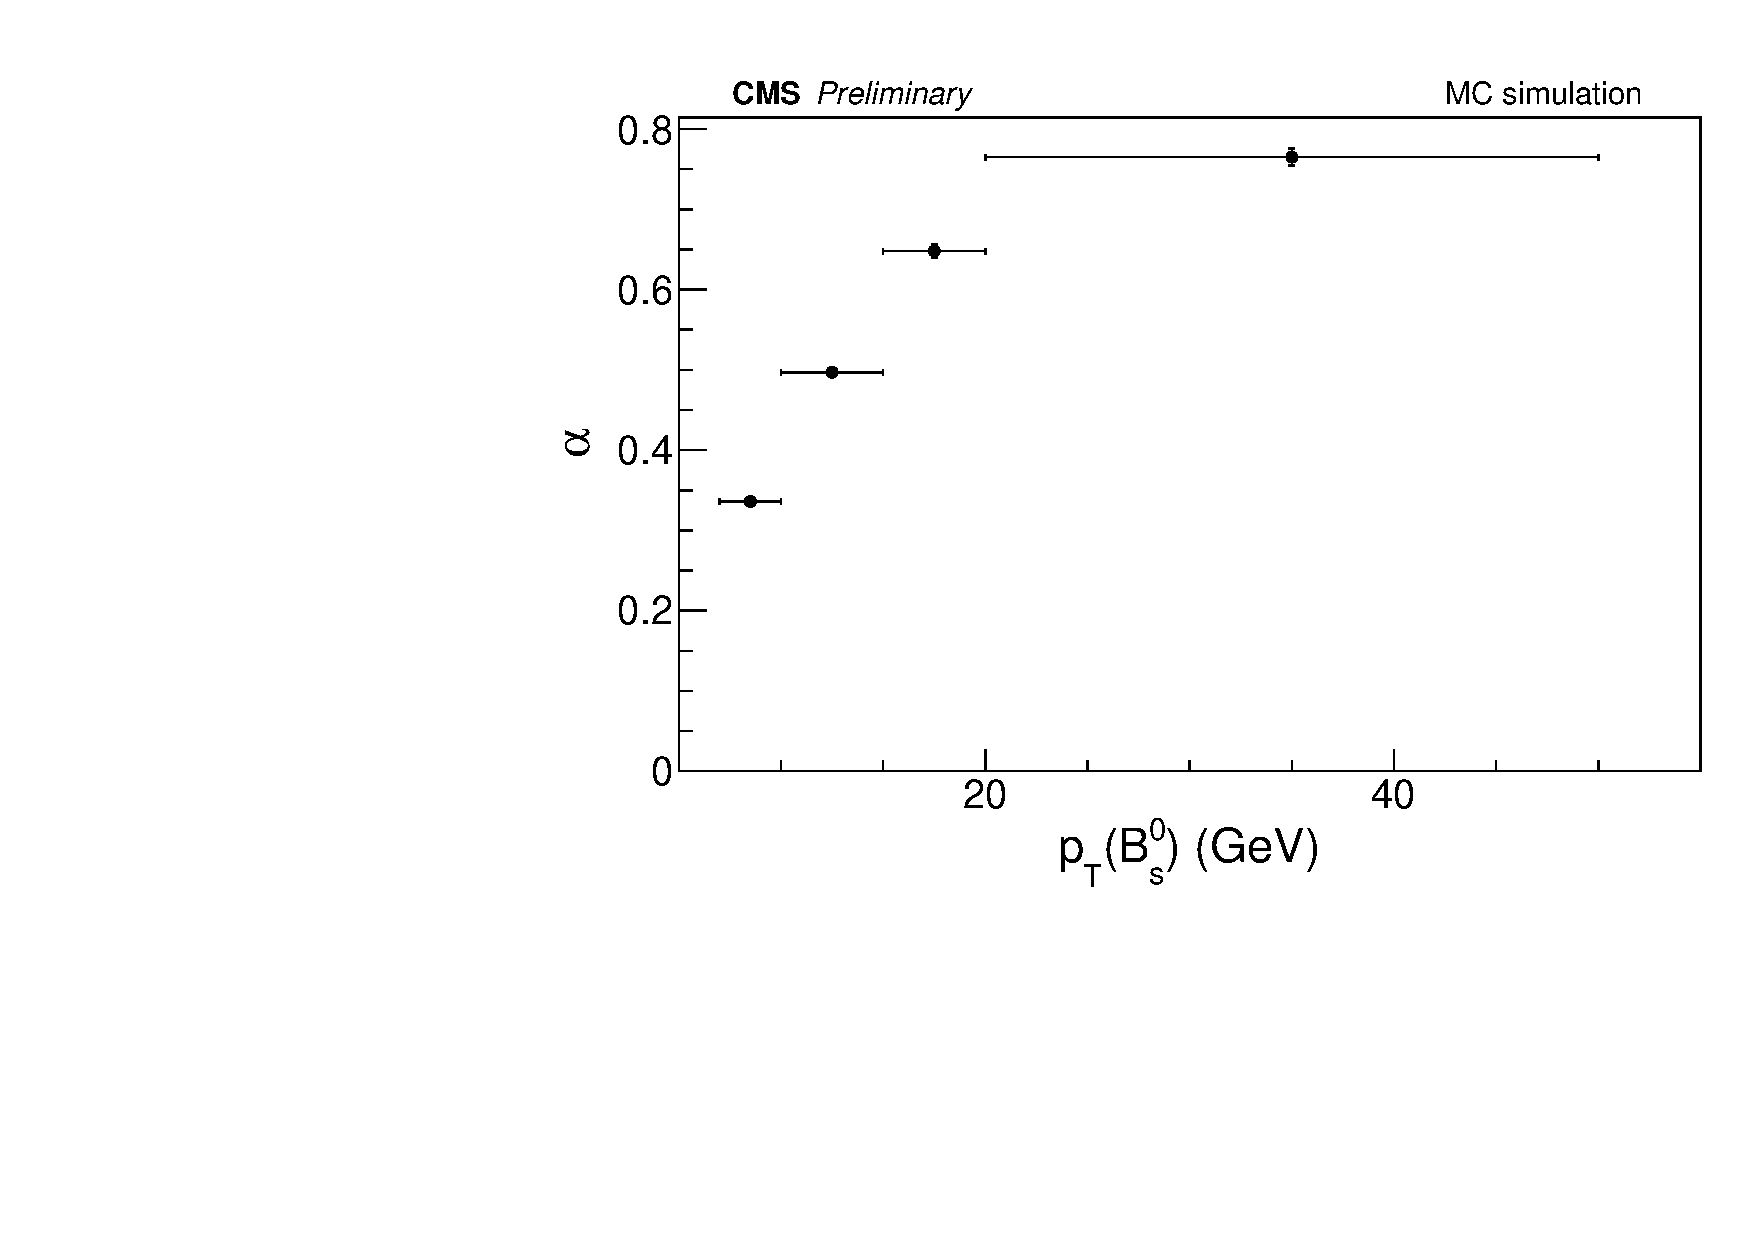
\includegraphics[width=\textwidth]{MainContent/Figs/effy/alpha_ptbins.PDF}
		\caption{}%
	\end{subfigure}
	\begin{subfigure}[b]{0.475\textwidth}
	\centering
	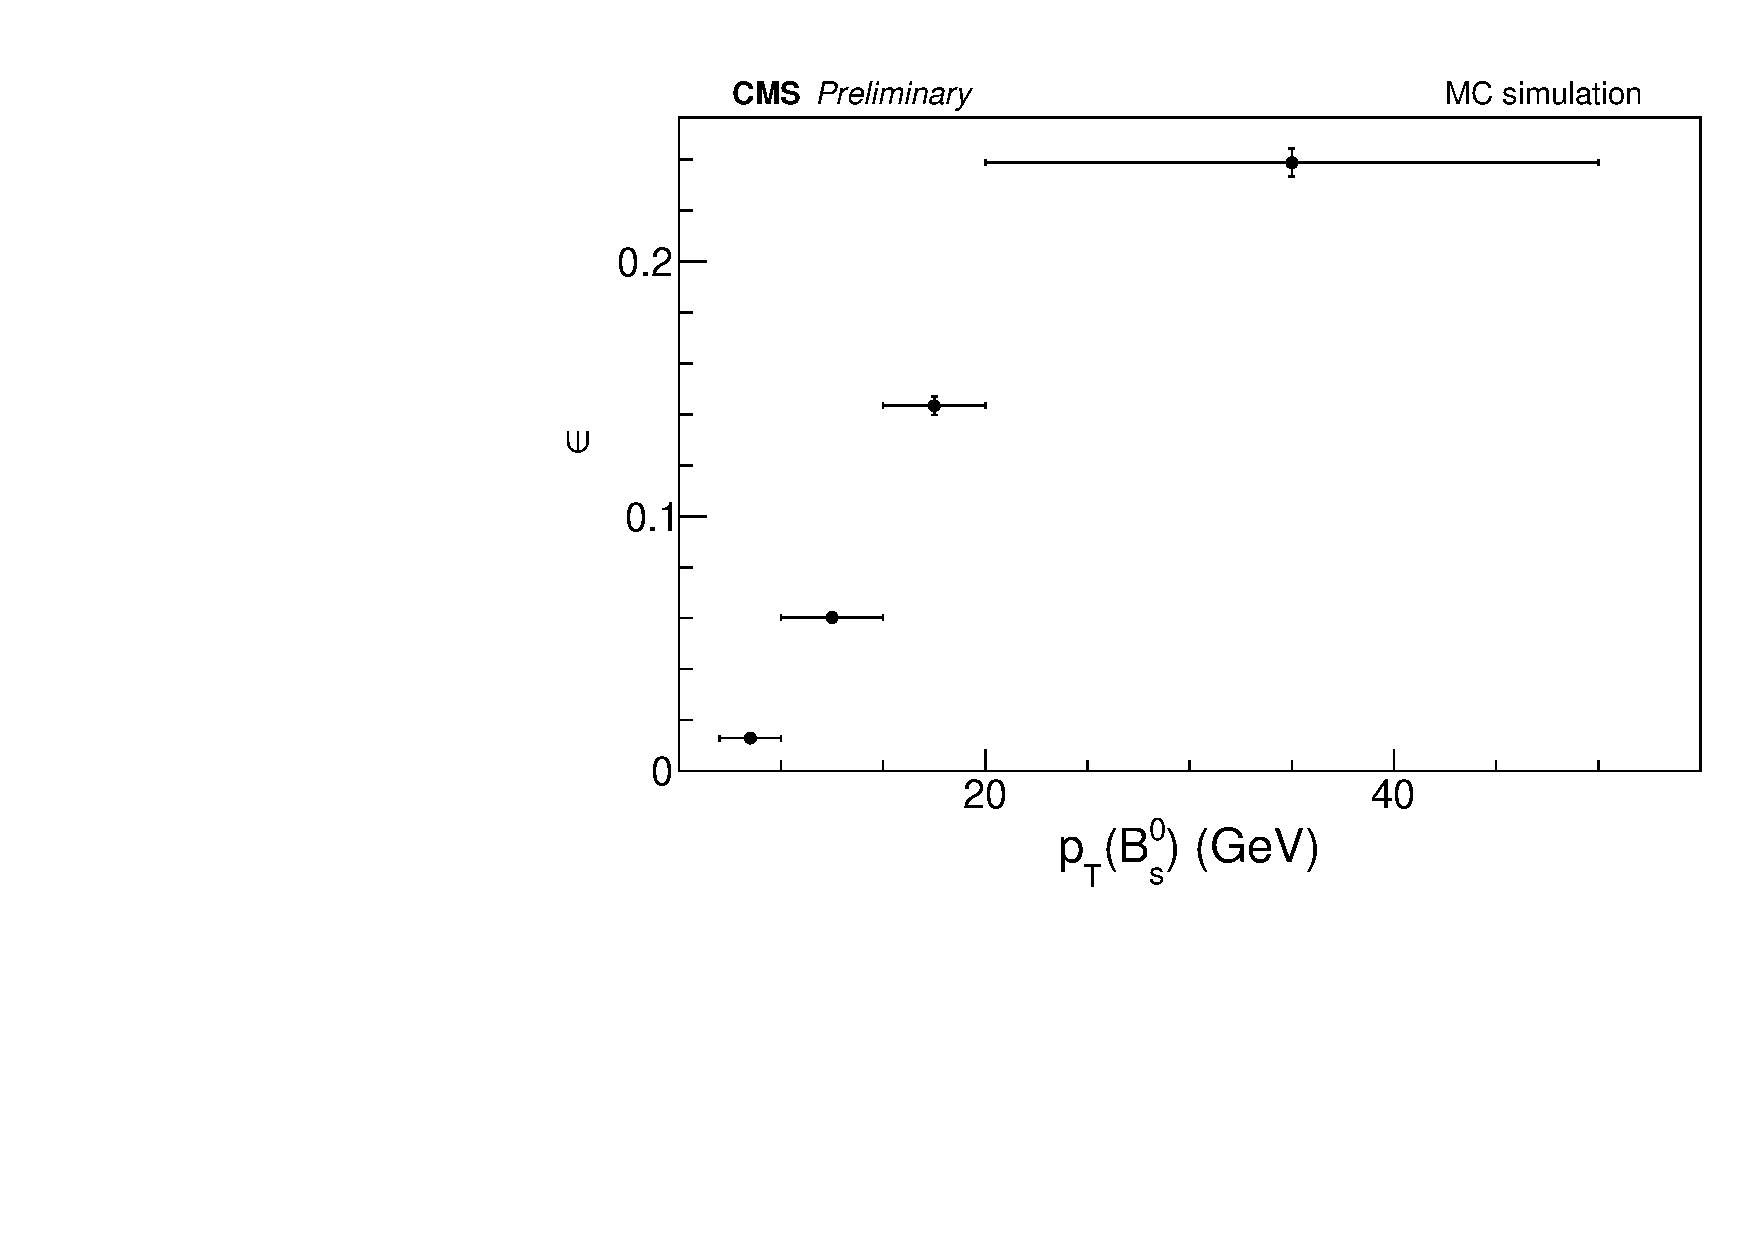
\includegraphics[width=\textwidth]{MainContent/Figs/effy/epsilon_ptbins.PDF}
	\caption{}%
\end{subfigure}
	\vskip\baselineskip
	\begin{subfigure}[b]{0.8\textwidth}
		\centering
		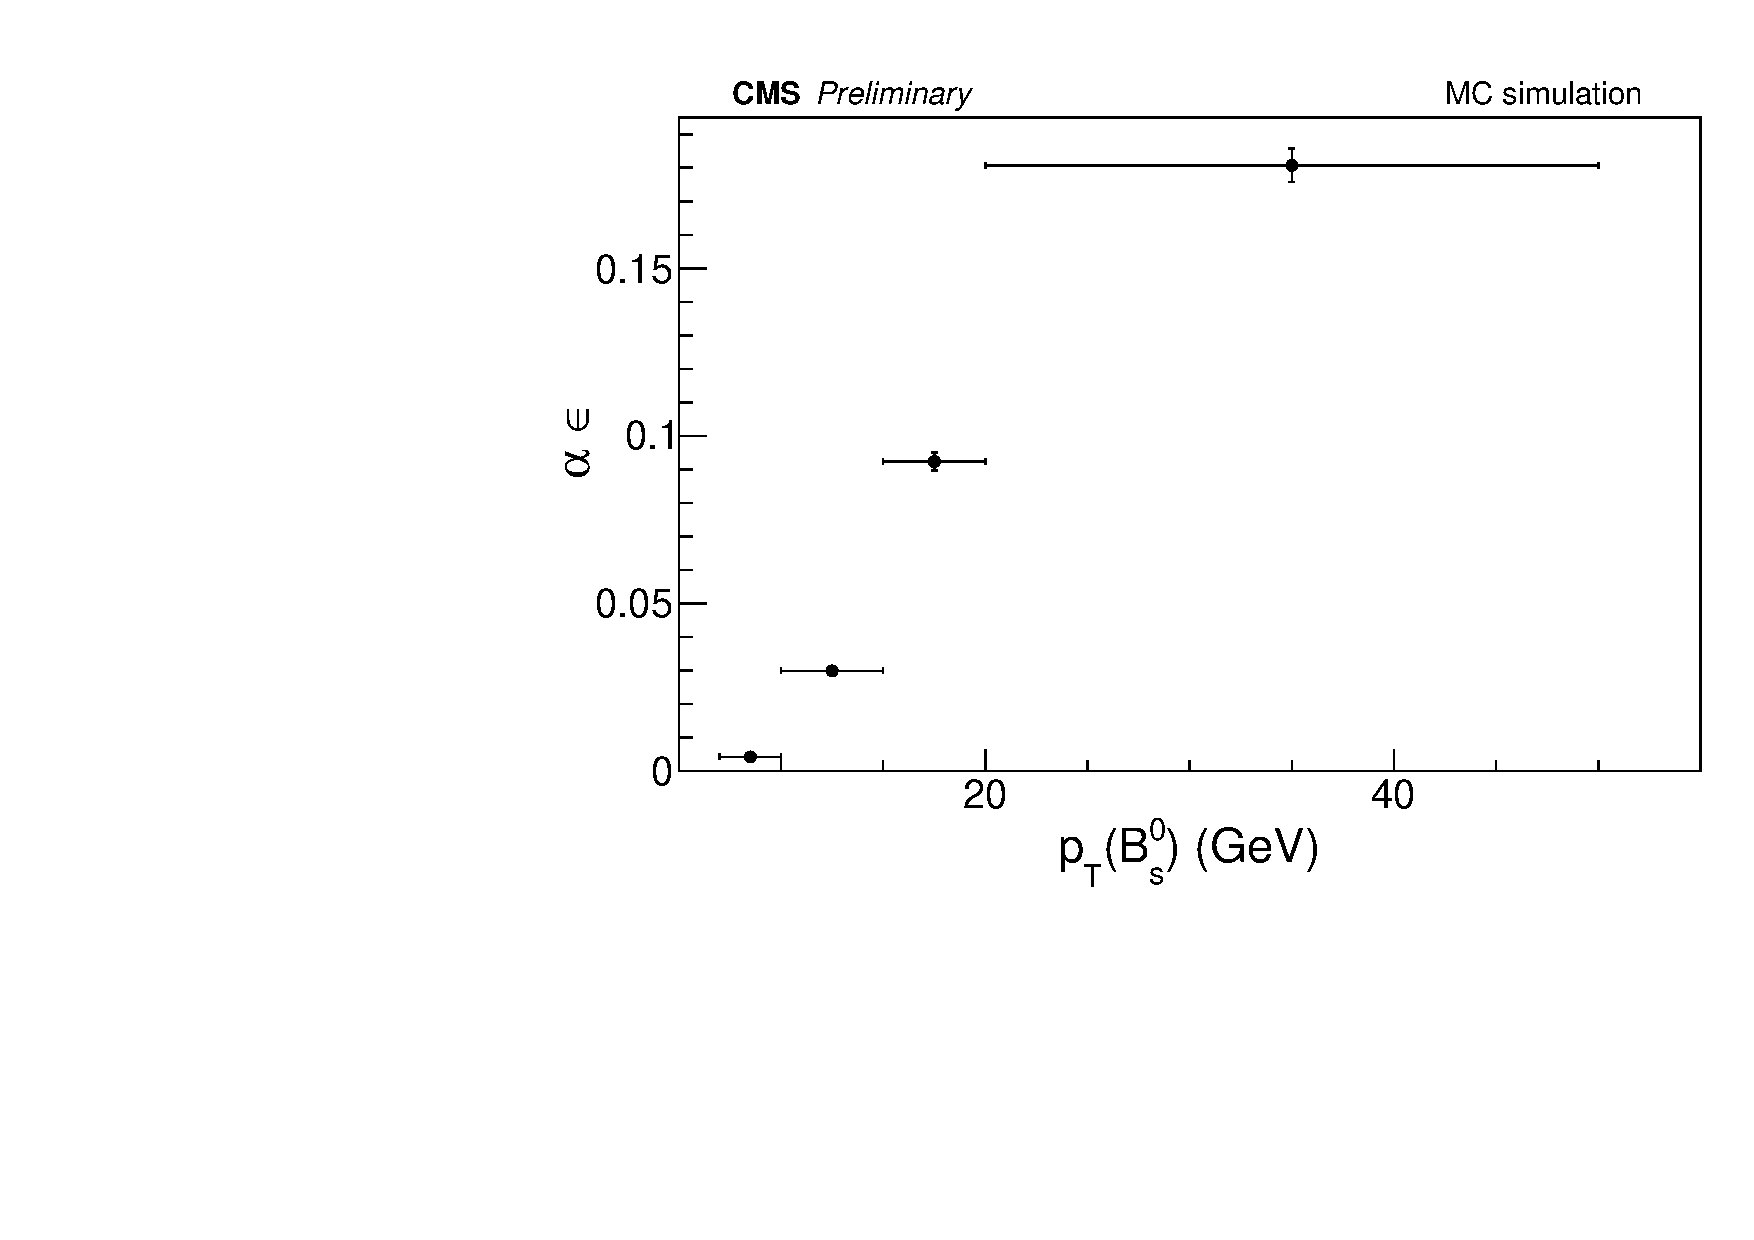
\includegraphics[width=\textwidth]{MainContent/Figs/effy/totaleffy_ptbins.PDF}
		\caption{}%
	\end{subfigure}
	\caption{(a) Acceptance, (b) efficiency and (c) total efficiency for the MC simulation using $p_T$ bins.}
	\label{fig:effy_ptbins}
\end{figure}

\begin{figure}[htp!]
	\centering
	\begin{subfigure}[b]{0.475\textwidth}
		\centering
		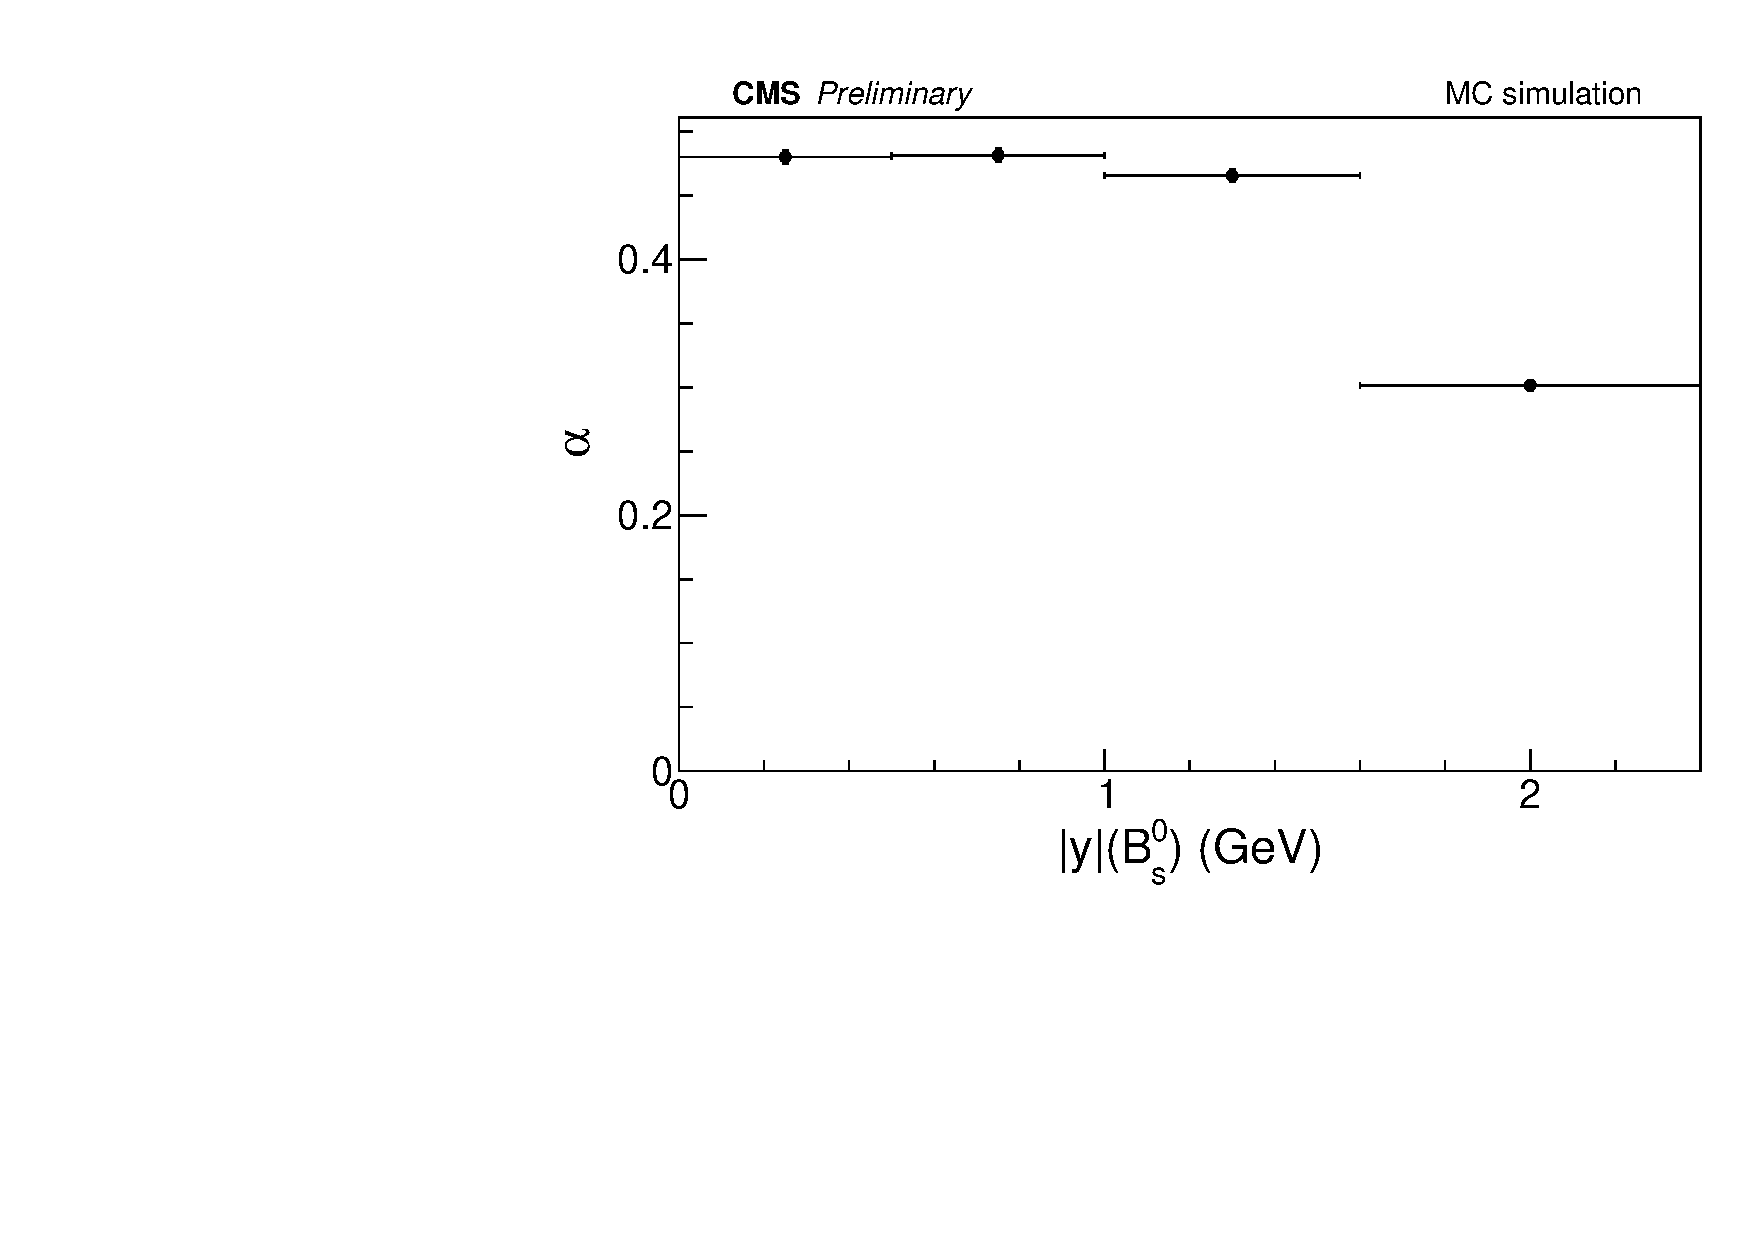
\includegraphics[width=\textwidth]{MainContent/Figs/effy/alpha_ybins.PDF}
		\caption{}%
	\end{subfigure}
	\begin{subfigure}[b]{0.475\textwidth}
		\centering
		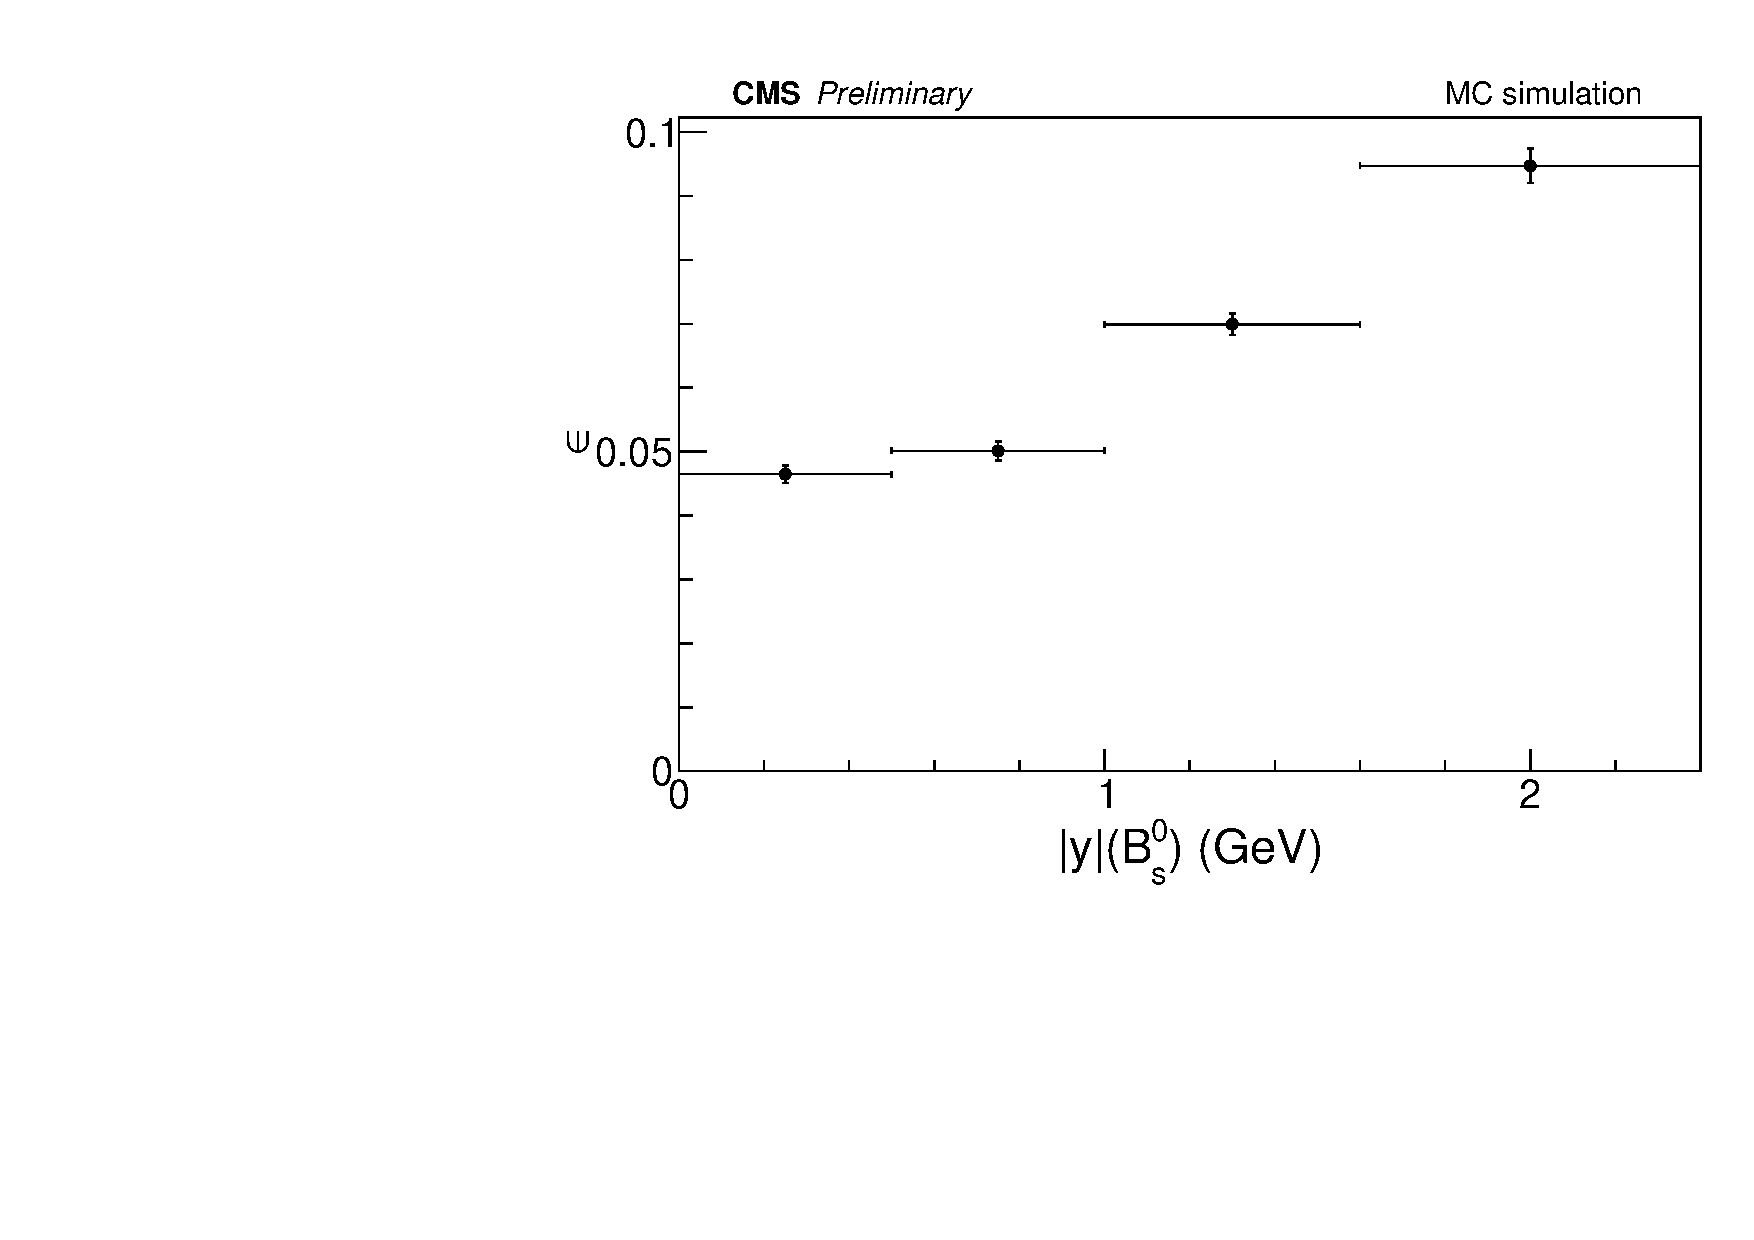
\includegraphics[width=\textwidth]{MainContent/Figs/effy/epsilon_ybins.PDF}
		\caption{}%
	\end{subfigure}
	\vskip\baselineskip
	\begin{subfigure}[b]{0.8\textwidth}
		\centering
		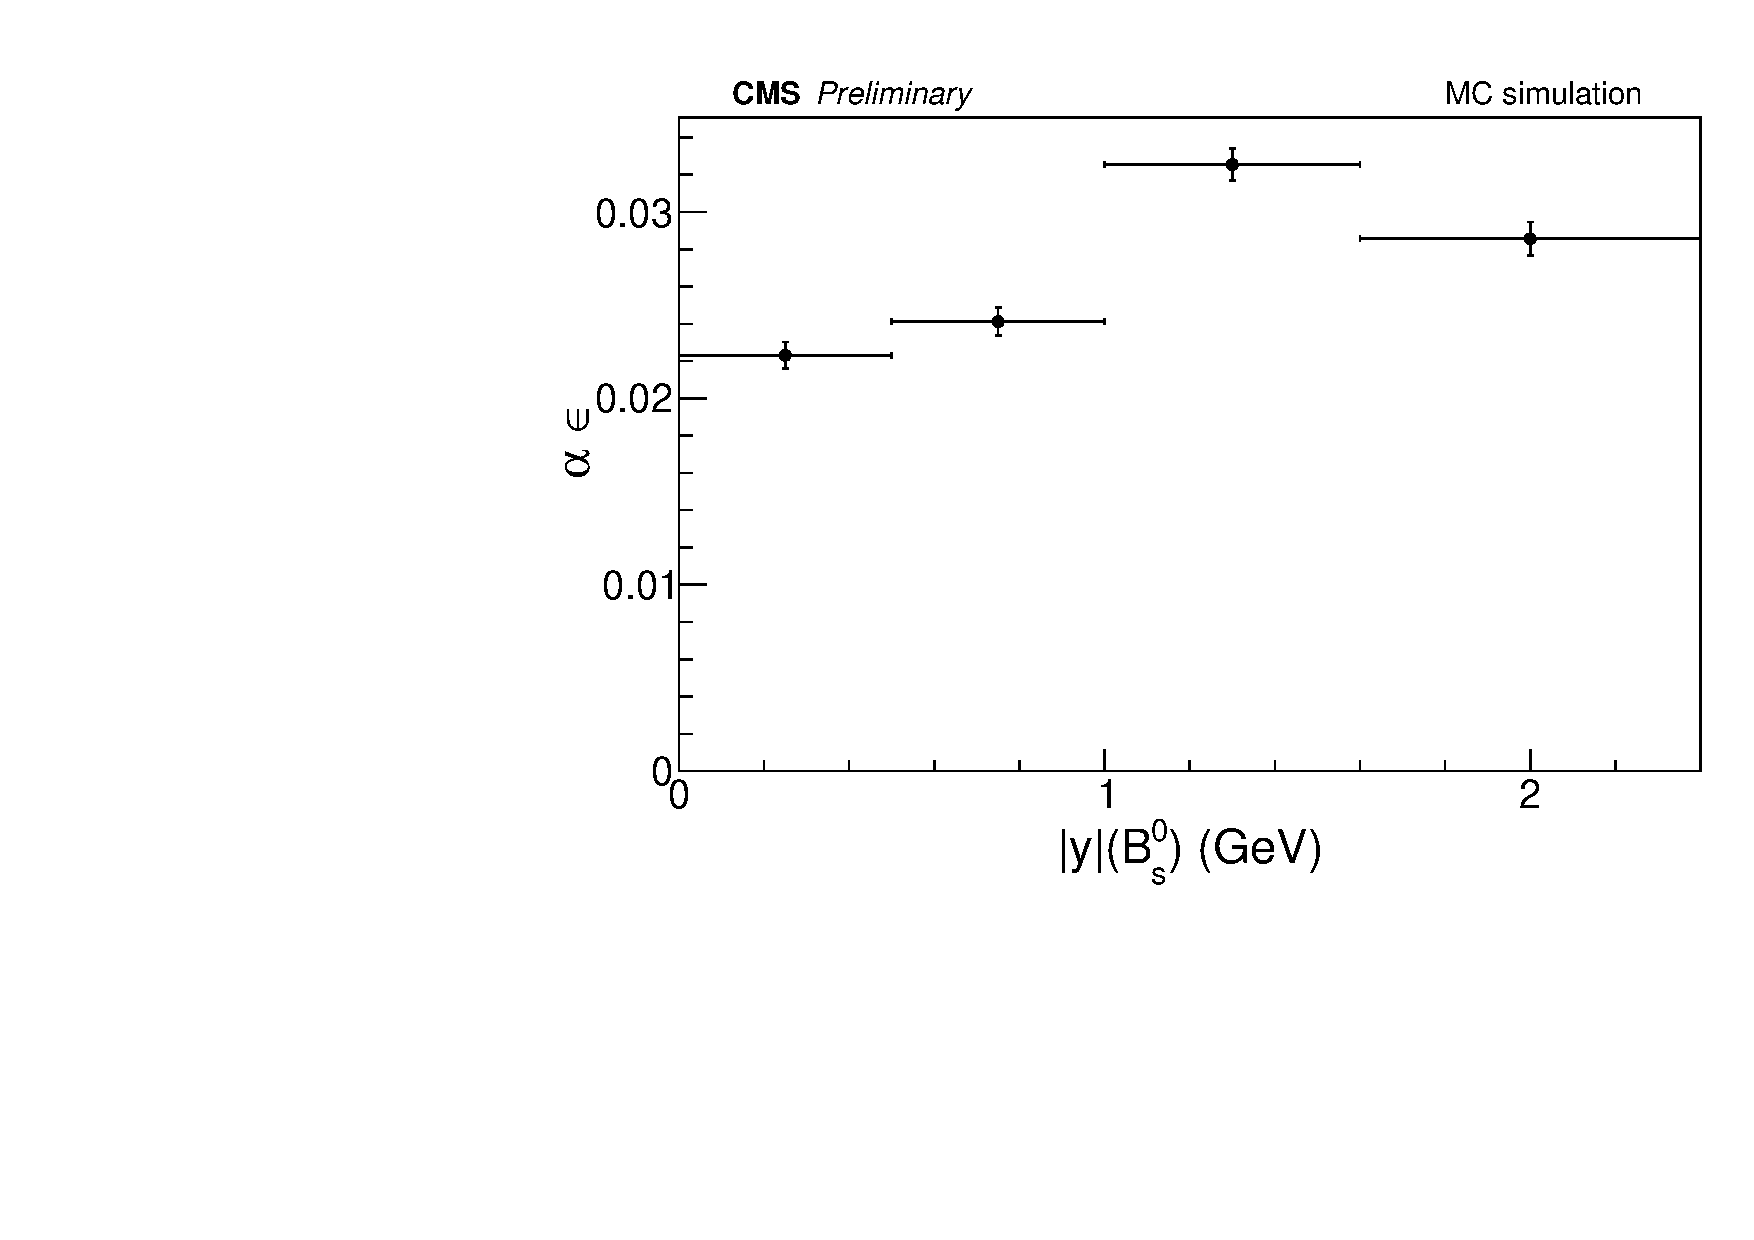
\includegraphics[width=\textwidth]{MainContent/Figs/effy/totaleffy_ybins.PDF}
		\caption{}%
	\end{subfigure}
	\caption{(a) Acceptance, (b) efficiency and (c) total efficiency for the MC simulation using $|y|$ bins.}
	\label{fig:effy_ybins}
\end{figure}

\section{Differential cross-section}

In particle physics, the term cross-section is used to express the probability of a given event occurring \cite{thomson2013modern}. More specifically, the probability that two colliding particles would interact and generate a certain event, such as the production of a specific particle \cite{pivarski2013}. The cross-section will be used in this thesis to refer to the probability of producing a $B^0_s$ meson during p-Pb collisions that decays in the manner described in \ref{subsec:channel}.

It is sometimes desirable to investigate how the cross-section is distributed with respect to a specific kinematic quantity  \cite{thomson2013modern}. This could be valuable in gaining a better understanding of the interaction. For this, the differential cross-section might be used. The differential cross-section with respect to the transverse momentum, $p_T$, is calculated as follows \cite{abe1995measurement}: 

\begin{equation}
	\label{eq:cs}
\frac{d \sigma(B_s^0 \to J/\psi\phi)}{dp_T} = \frac{N_{B^0_s}}{2 \Delta p_T \cdot \alpha \cdot \epsilon \cdot BR \cdot \mathcal{L}}
\end{equation}

where $\Delta p_T$ is the width of the $p_T$ region, $\alpha \cdot \epsilon$ is the total efficiency, BR is the branching ratio of the total decay chain, eq. \ref{eq:br}, and $\mathcal{L} = 179.7$ nb$^{-1}$  is the total integrated luminosity. Due to the quick transitions between particle and antiparticle, indicated in \ref{sec:b0s}, both $B^0_s$ and $\bar{B^0_s}$ are formed in the collision, but only $B^0_s$ is considered, for this reason, the factor $\frac{1}{2}$ is included in the equation above. Similarly, the differential cross-section for the $|y|$ bins is defined as: 

\begin{equation}
	\label{eq:cs_y}
	\frac{d \sigma(B_s^0 \to J/\psi\phi)}{d|y|} = \frac{N_{B^0_s}}{2 \Delta |y| \cdot \alpha \cdot \epsilon \cdot BR \cdot \mathcal{L}}
\end{equation}

Table \ref{table:result_raw_fdfu} shows the number of signal events, the total reconstruction efficiency and the value for the differential cross-section for the different $p_T$ bins. The top of Fig. \ref{fig:cs} depicts the results of the $p_T$ differential cross-section. The plot shows a comparison with the fixed-order plus next-to-leading-logarithm (FONLL) predictions \cite{FONLL}. The FONLL data has been calculated for pp collisions and the $B$ meson. A data escalation was performed by multiplying by the number of nucleons in the Pb nucleus, 208, and by the world average $B^{0}_s$ production fraction, $10.0 \%$ \cite{khachatryan2016study, pdgadmixture}. The error bars for the calculated differential cross-section represent systematic and statistical uncertainty. These will be discussed further in the following section. Table \ref{table:mc_ybins} and fig. \ref{fig:cs_y} show the results for the $|y|$ bins. 

\begin{table}[htbp] \begin{center}\begin{tabular}{|c|c|c|c|}\hline\textbf{$\mathbf{p_T}$ bin (GeV)} & \textbf{$\mathbf{N_{B_s^{0}}}$} & \textbf{$\mathbf{B_s^{0}}$ Total Efficiency} & \textbf{${\mathbf{\frac{d \sigma}{dp_T}}}$ ($\mu$b/GeV)} \\\hline{[}7, 10{)} &  56  $\pm$  8 &   0.0044  $\pm$  0.0002 &   375.37  $\pm$  55.77 \\{)}10, 15{)} &  116  $\pm$  12 &   0.0300  $\pm$  0.0008 &   68.17  $\pm$  6.93 \\{[}15, 20{)} &  89  $\pm$  10 &   0.0929  $\pm$  0.0026 &   16.74  $\pm$  1.92 \\{[}20, 50{)} &  104  $\pm$  11 &   0.1826  $\pm$  0.0049 &   1.67  $\pm$  0.18 \\\hline\end{tabular}\caption{The $N_{B_s^{0}}$ values obtained and efficiencies computed are shown with their respective statistical uncertainties. The value of ${\frac{d \sigma}{dp_T}}$ computed directly from these results is also shown. For ${\frac{d \sigma}{dp_T}}$, just the $N_{B_s^{0}}$ error propagation is present.}\label{table:result_raw_fdfu}\end{center}\end{table}

\begin{table}[htbp] \begin{center}\begin{tabular}{|c|c|c|c|}\hline\textbf{$\mathbf{|y|}$ bin (GeV)} & \textbf{$\mathbf{N_{B_s^{0}}}$} & \textbf{$\mathbf{B_s^{0}}$ Total Efficiency} & \textbf{${\mathbf{\frac{d \sigma}{d|y|}}}$ ($\mu$b/GeV)} \\\hline{[}0.0, 0.5{)} &  71  $\pm$  9 &   0.0223  $\pm$  0.0007 &   556.21  $\pm$  68.54 \\{[}0.5, 1.0{)} &  72  $\pm$  9 &   0.0241  $\pm$  0.0007 &   522.83  $\pm$  65.87 \\{)}1.0, 1.6{)} &  126  $\pm$  12 &   0.0325  $\pm$  0.0008 &   568.55  $\pm$  54.33 \\{[}1.6, 2.4{)} &  100  $\pm$  12 &   0.0286  $\pm$  0.0009 &   385.95  $\pm$  45.13 \\\hline\end{tabular}\caption{The $N_{B_s^{0}}$ values obtained and efficiencies computed are shown with their respective statistical uncertainties. The value of ${\frac{d \sigma}{d|y|}}$ computed directly from these results is also shown. For ${\frac{d \sigma}{d|y|}}$, just the $N_{B_s^{0}}$ error propagation is present.}\label{table:result_raw_fdfu_y}\end{center}\end{table}


It is observed that the in the center region of $p_T$, $[10, 20)$ GeV, the experimental data is closer to the FONLL prediction than in the regions of lower $p_T$, $[7, 10)$ GeV and higher $p_T$, $[20, 50)$ GeV. Nevertheless, when the double of the uncertainty for both FONLL and the experimental data is taken into account, the values fall into the $95\%$ \cite{vsirca2016probability} confidence interval. The FONLL prediction for a wider range of values is shown in the bottom of Fig. \ref{fig:cs}. The data is fitted with a curve. The total $p_T$ differential cross-section is estimated as $\frac{d \sigma}{dp_T} = (24.834 \pm 1.435(stat) \pm 5.680(sys)) \ \mu\text{b}/\text{GeV}$.

On the other hand, when considering the rapidity $|y|$, the values from FONLL and the experimental results agree when considering the total uncertainty. The value of the total $|y|$ differential cross-section is 
$\frac{d \sigma}{d|y|} = (507.34 \pm 29.31(stat) \pm 115.54(sys)) \ \mu\text{b}/\text{GeV}$.
\begin{figure*}
	\centering
	\begin{subfigure}[b]{0.7\textwidth}
		\centering
		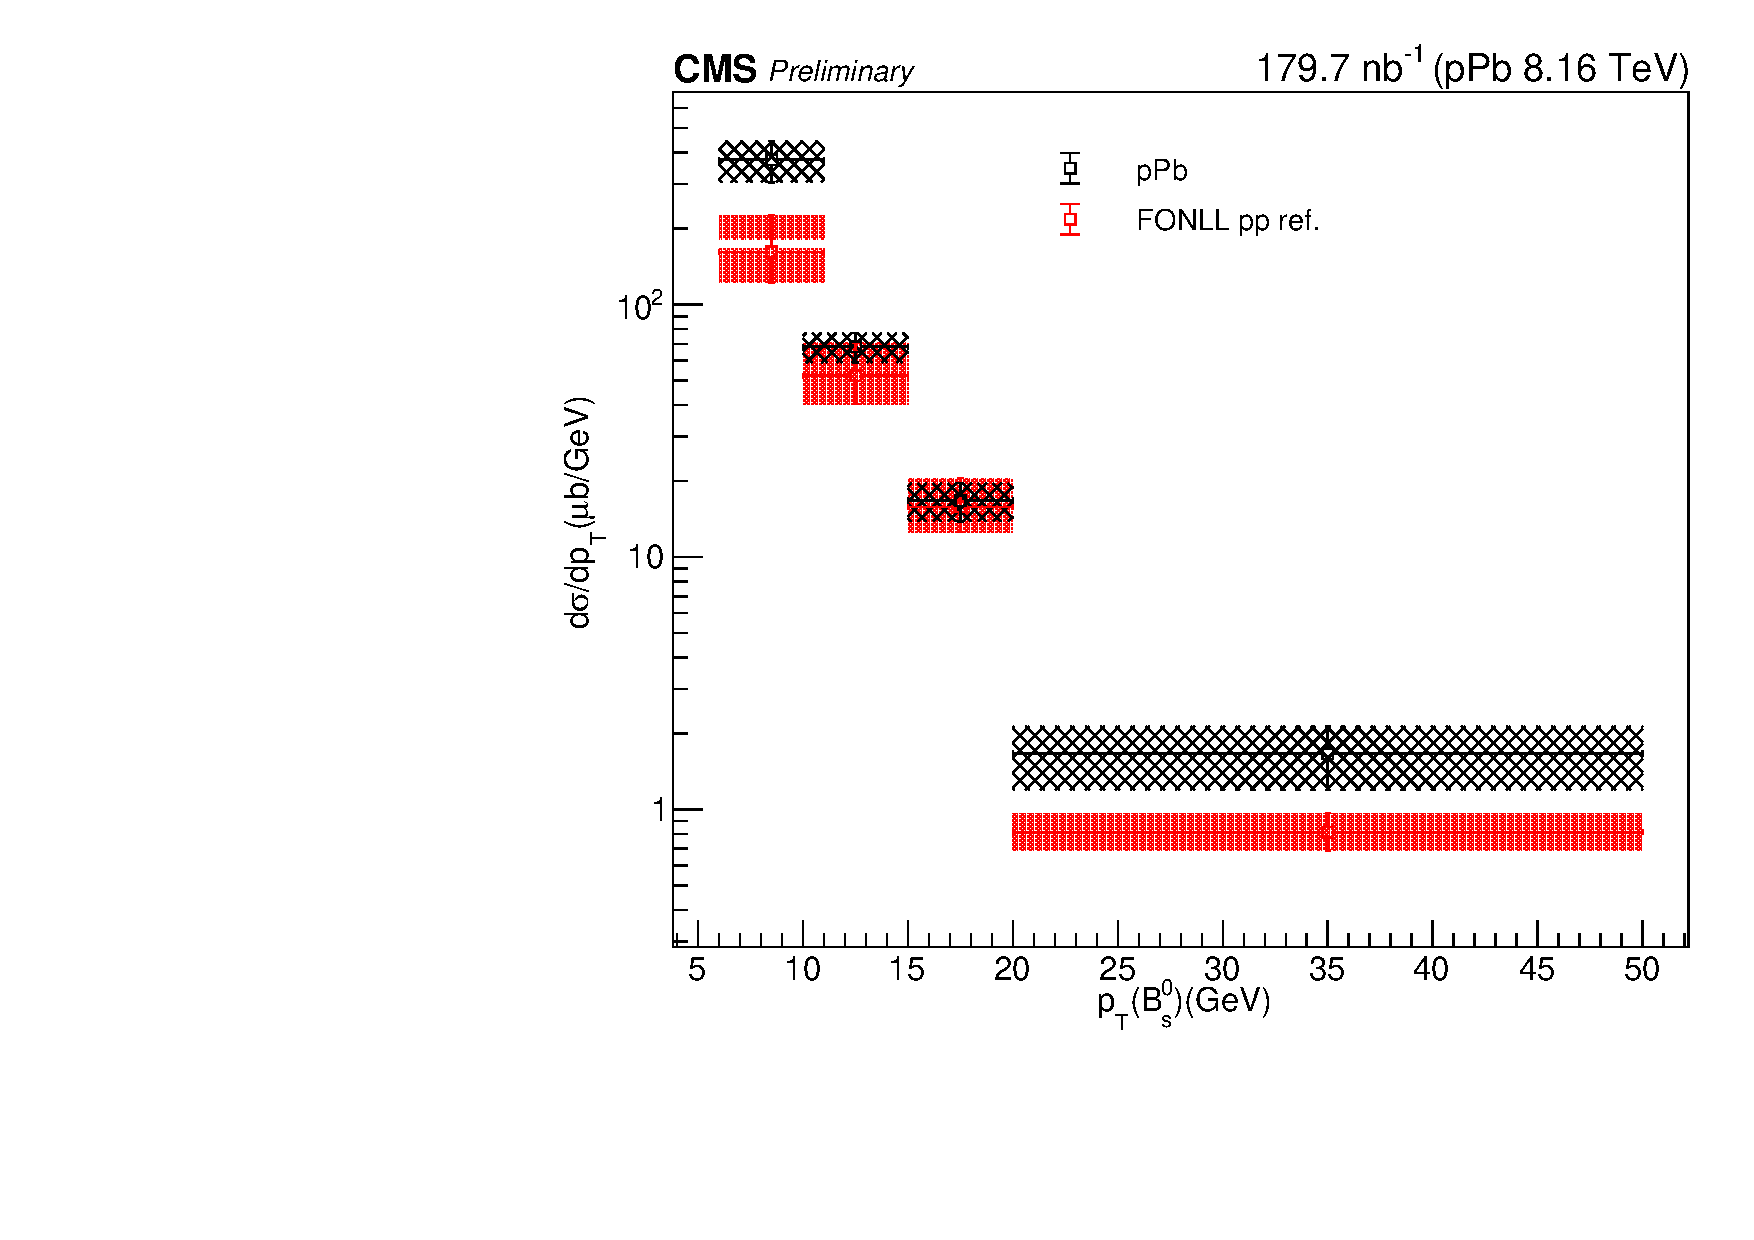
\includegraphics[width=\textwidth]{MainContent/Figs/effy/Histo_Bs_CS_pt_FONLL_8Tev.PDF}
		\caption{}%
	\end{subfigure}
	\vskip\baselineskip
	\begin{subfigure}[b]{0.7\textwidth}
		\centering
		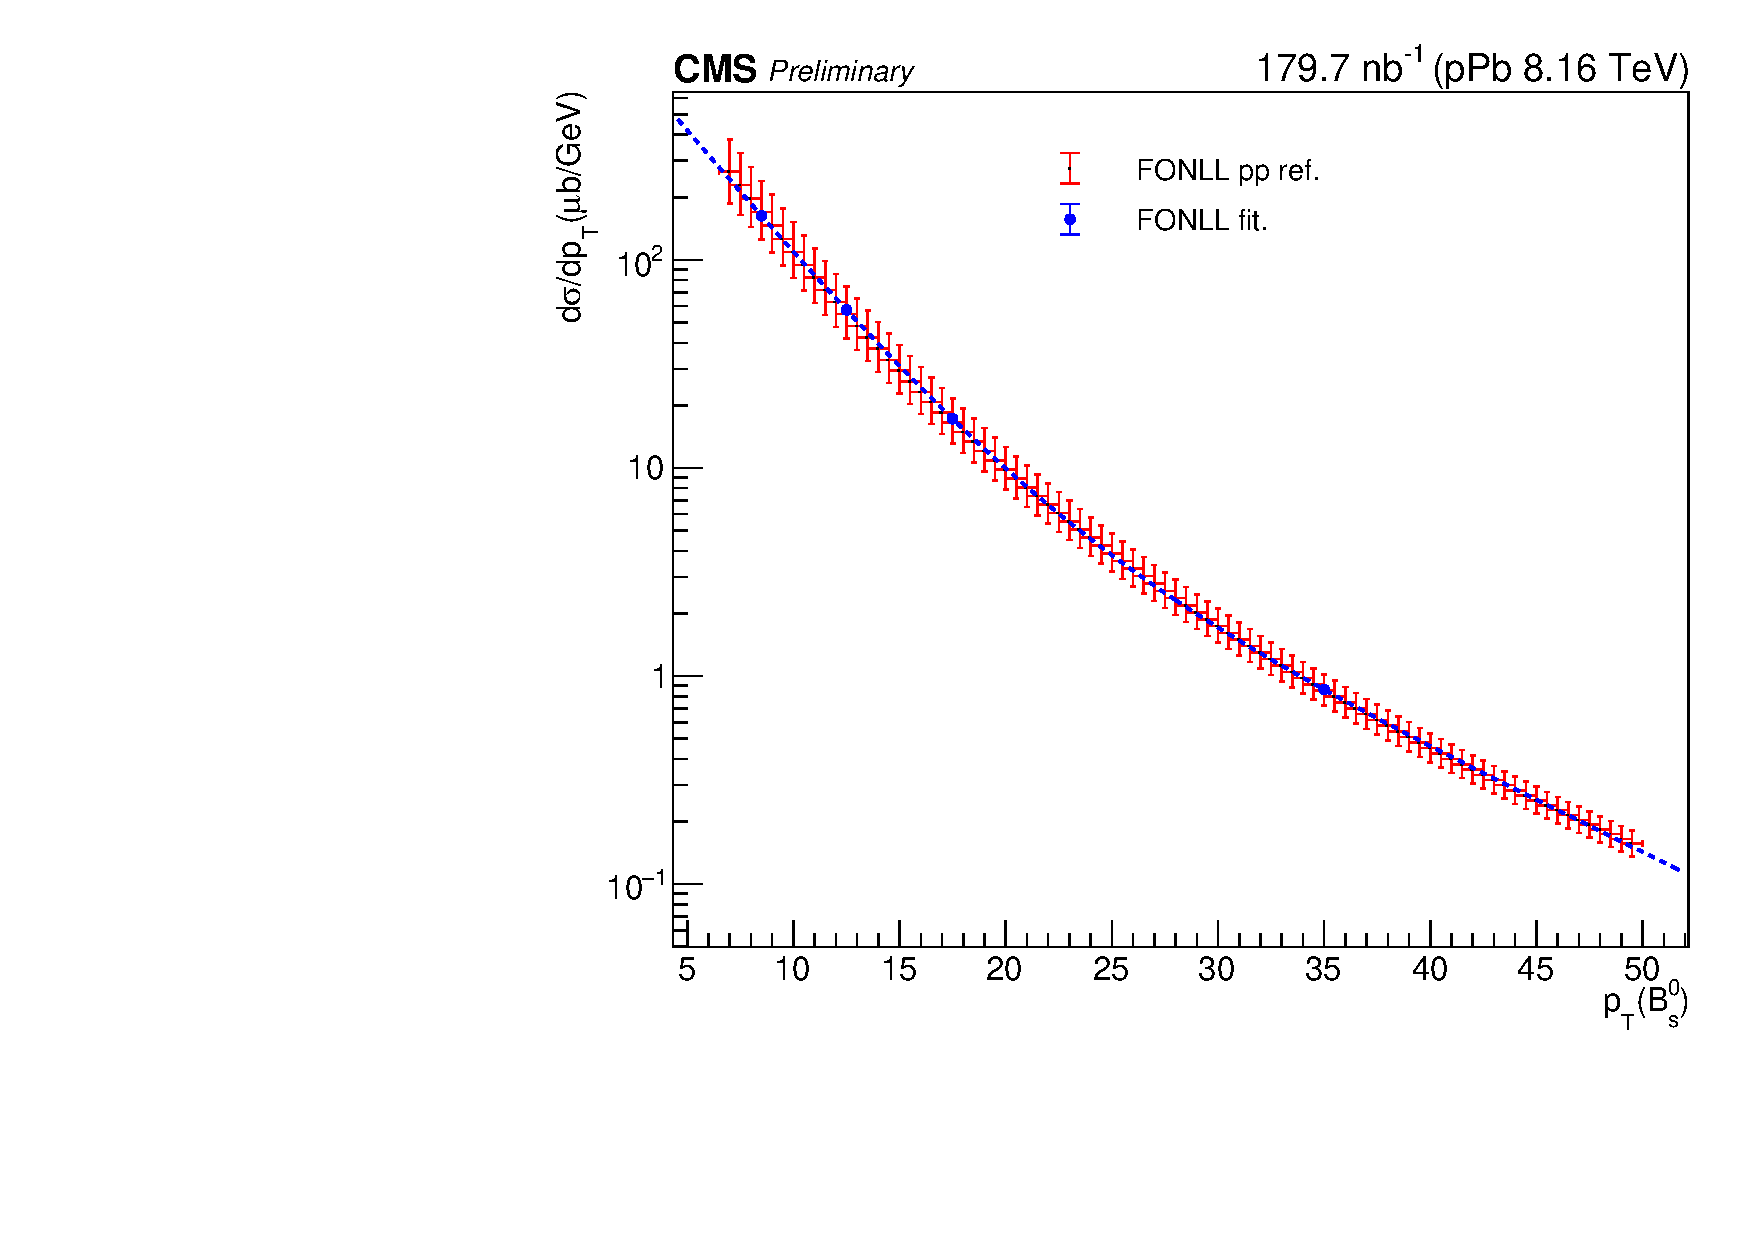
\includegraphics[width=\textwidth]{MainContent/Figs/effy/Histo_Bs_CS_pt_FONLL_8Tev_curve.PDF}
		\caption{}%
	\end{subfigure}
	\caption{$p_T$ Differential cross-section for the $B^0_s$ meson, where a) corresponds to a comparison between predicted and calculated values and b) full plot of predicted values.}
	\label{fig:cs}
\end{figure*}

\begin{figure*}
	\centering
	\begin{subfigure}[b]{0.7\textwidth}
		\centering
		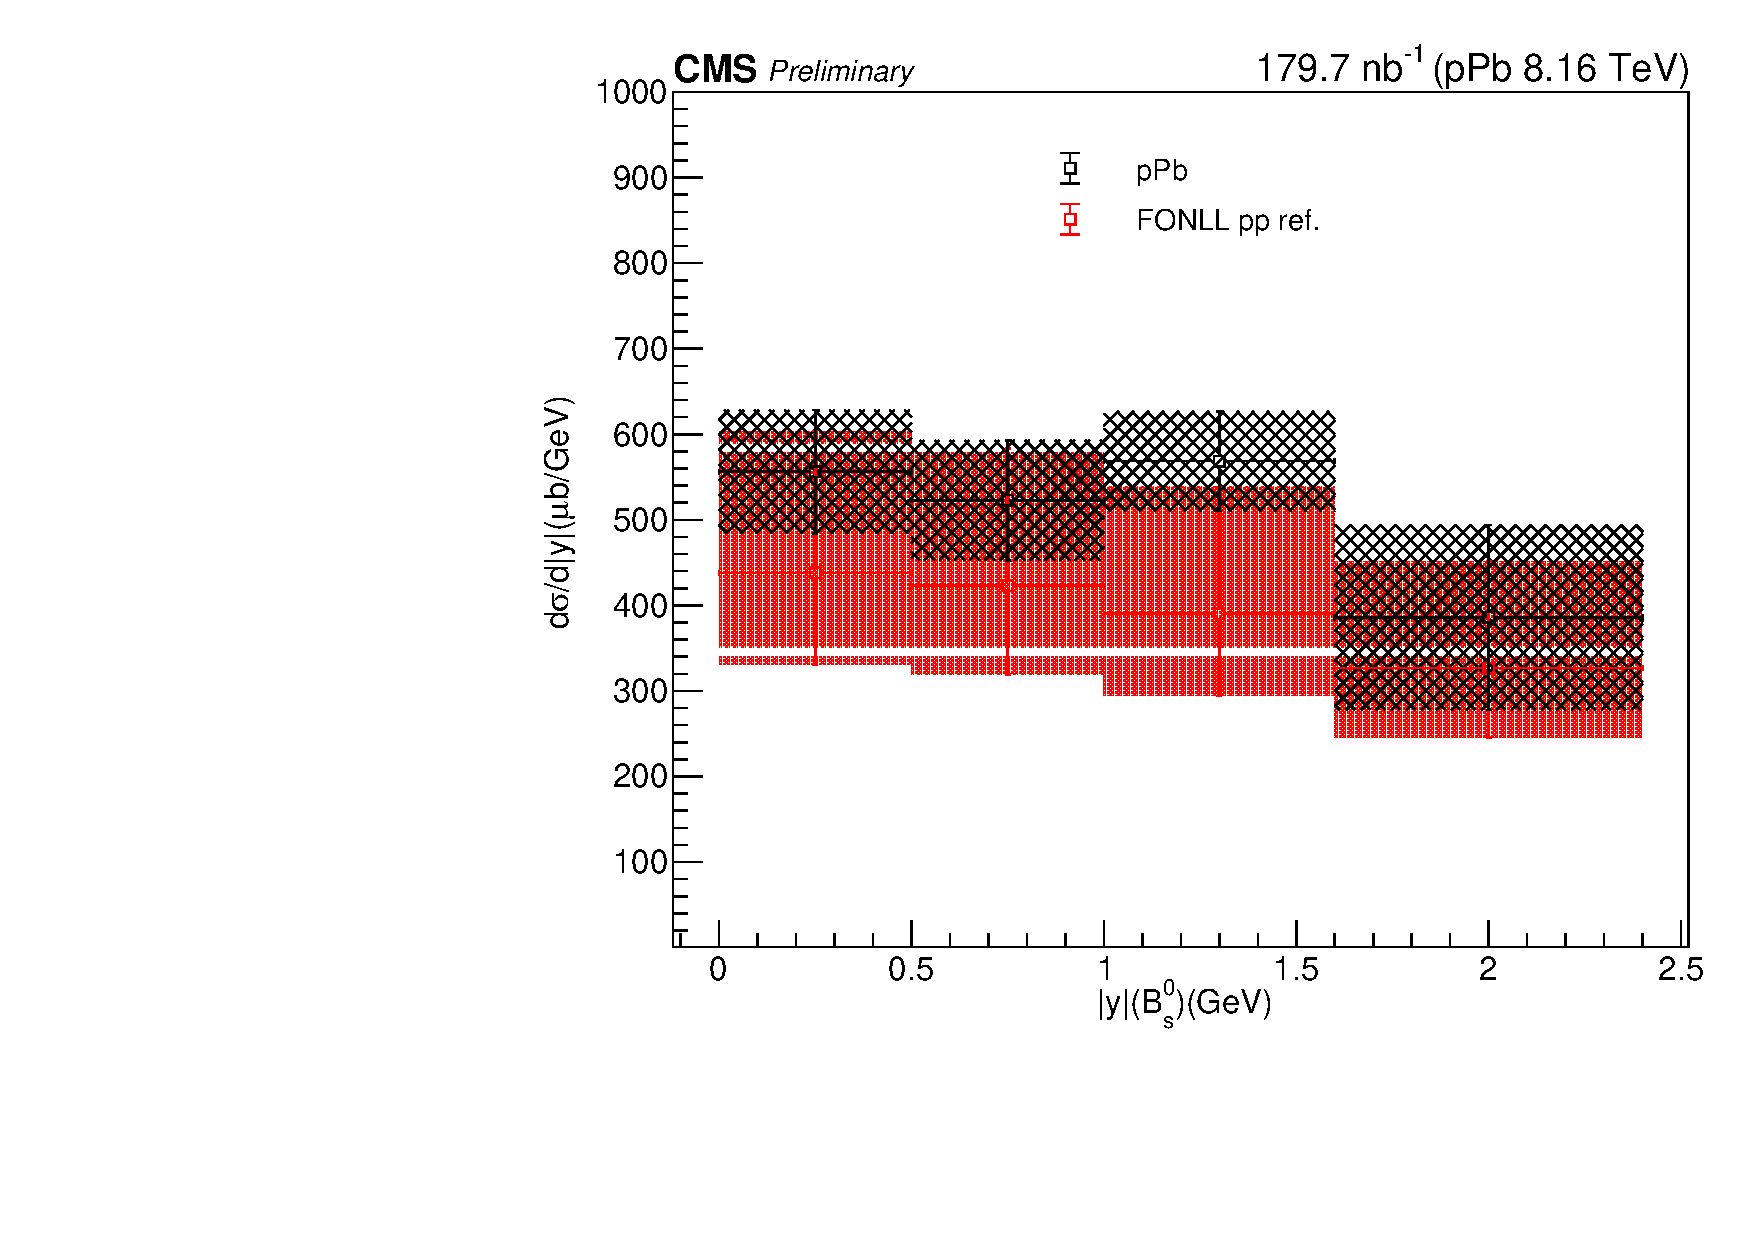
\includegraphics[width=\textwidth]{MainContent/Figs/effy/Histo_Bs_CS_y_FONLL_8Tev.PDF}
		\caption{}%
	\end{subfigure}
	\vskip\baselineskip
	\begin{subfigure}[b]{0.7\textwidth}
		\centering
		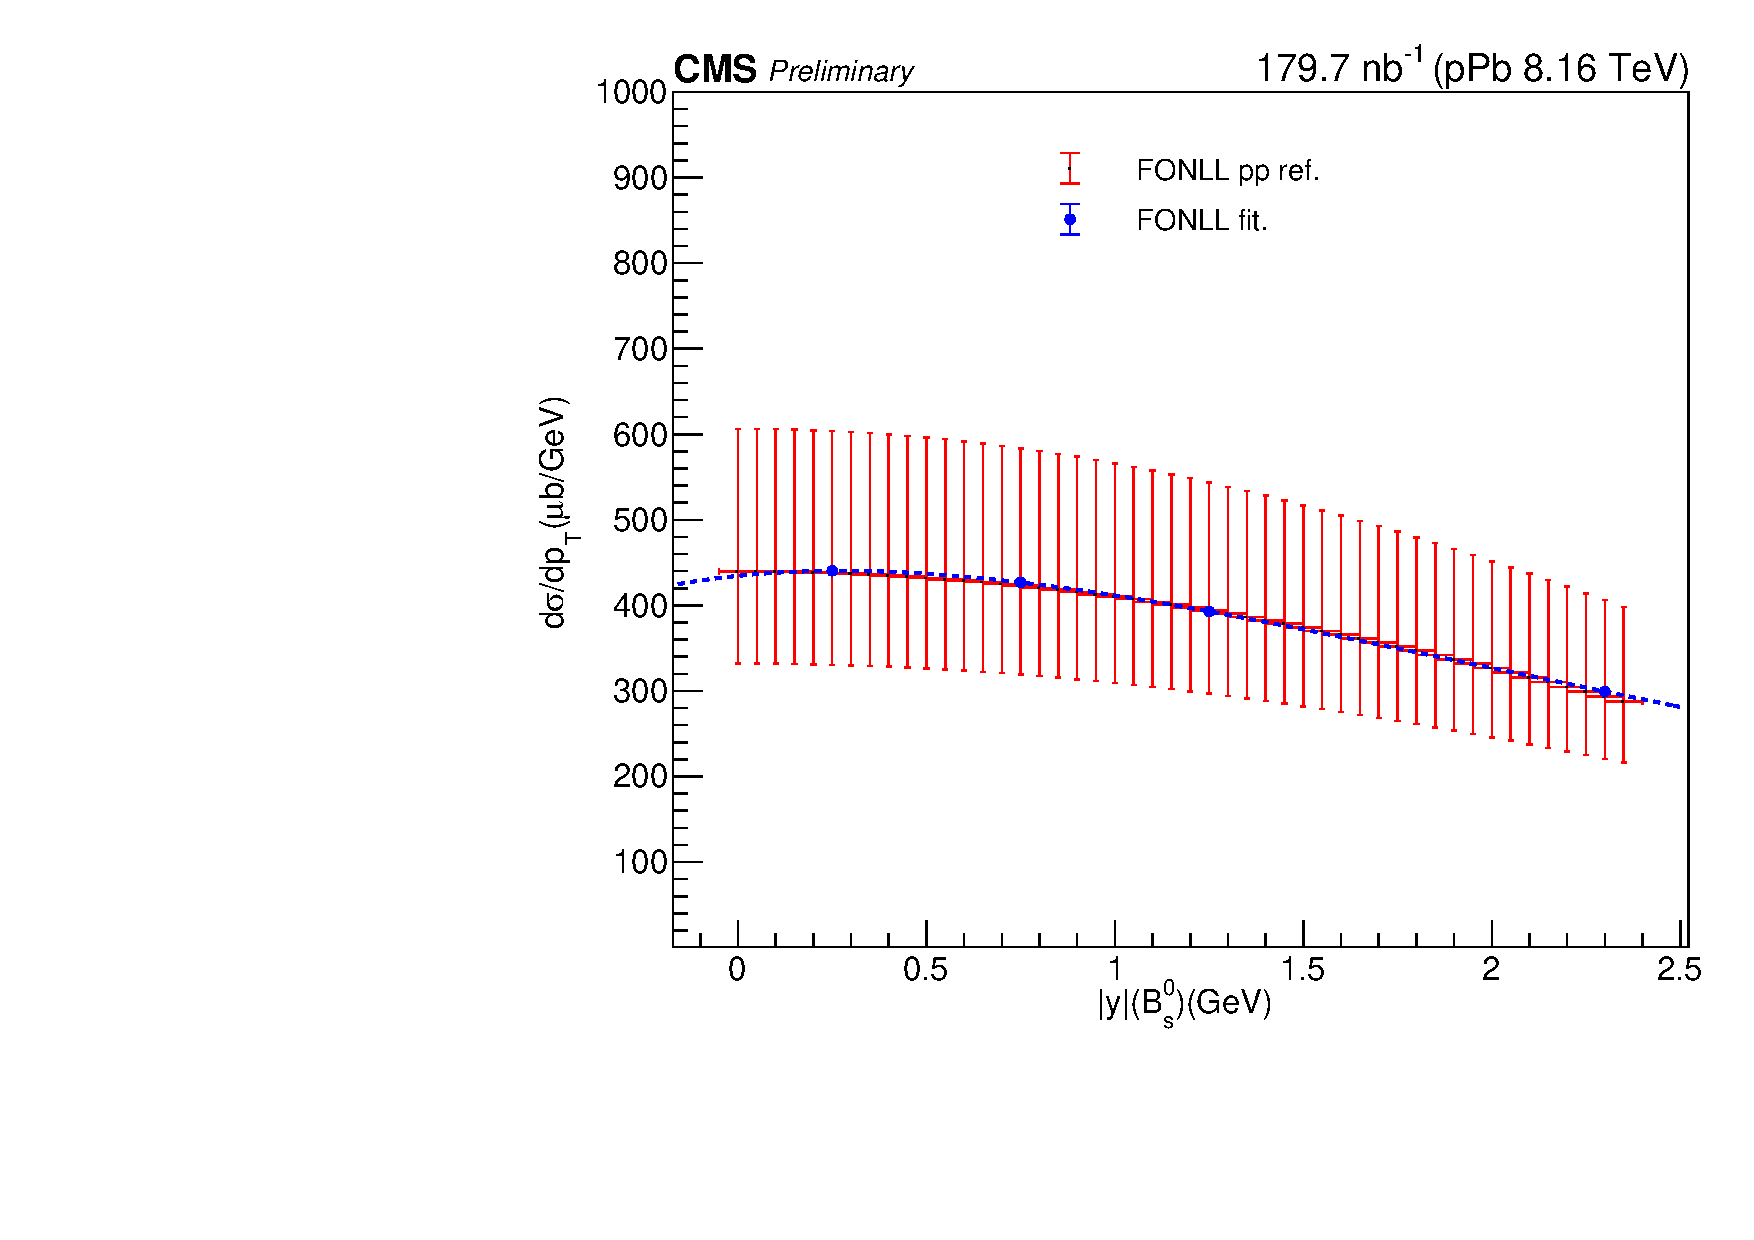
\includegraphics[width=\textwidth]{MainContent/Figs/effy/Histo_Bs_CS_y_FONLL_8Tev_curve_ybins.PDF}
		\caption{}%
	\end{subfigure}
	\caption{$|y|$ differential cross-section for the $B^0_s$ meson, where a) corresponds to a comparison between predicted and calculated values and b) full plot of predicted values.}
	\label{fig:cs_y}
\end{figure*}

 \cleardoublepage
\section{Uncertainty in the differential cross-section}
The uncertainties in the measurement of a quantity during a physics experiment can be classified by two types. The first type are the statistical uncertainties, which are related to the fact that multiple measurements of the same quantity can yield different results. Therefore, the value of such quantity is not precise, but fluctuates within a range. The measurement of this range is the statistical uncertainty \cite{sinervo2003definition}. The statistical uncertainties are calculated by \verb|ROOTFIT|, and in the case of the ML method, these are determined by the covariance matrix $\mathrm{var}[\vec{\Theta}]$ \cite{vsirca2016probability}:

\begin{equation}
	\mathrm{var}[\vec{\Theta}] = 
	\left(-E\left[ \frac{\partial^2 l(x | \vec{\Theta}) }{\partial \vec{\Theta} ^2}\right]_{\Theta = \hat{\Theta}}\right)^{-1}
\end{equation}

with $E[X]$ the expected value of $X$. The diagonals are the variance of the parameters $\vec{\Theta}$ and the uncertainty is the square root of the variance, 

\begin{equation}
	\delta \Theta_i = \sqrt{\mathrm{var}[\Theta_i]}
\end{equation}

On the other hand, given a set of $N$ random variables $\vec{X}$ and a respective covariance matrix $\mathrm{var}[\vec{X}]$, if a function $f = f(\vec{X})$ depends on these variables, then the variance associated to $f$ is calculated by \cite{vsirca2016probability}:

\begin{equation}
	\mathrm{var}[f(\vec{X})] = \sum_{i=1}^N \sum_{j=1}^N \left(\frac{\partial f}{\partial X_i} \frac{\partial f}{\partial X_j} \right)_{X = \mu} \mathrm{var}[\vec{X}]_{i,j}
\end{equation}

with the partial derivatives evaluated at the mean value of $X$, $\mu$. When there is no correlation between variables, the previous equation reduces to:

\begin{equation}
	\label{totaluncertainty}
	\mathrm{var}[f(\vec{X})] = \sum_{i=1}^N  \left(\frac{\partial f}{\partial X_i}\right)^2_{X = \mu} \mathrm{var}[X_i]
\end{equation}

Revise \cite{vsirca2016probability} for more information on expected values, variance, and their relation to uncertainties. Alternatively, any statistical book on the subject would suffice.

The second type are systematic uncertainties. They are related to the nature of the instrument used, the specific model chosen for the data, the assumptions made about the experiment beforehand, among other factors. It should be noted that by taking more measurements of the quantity, the value of the statistical uncertainty can be minimized. For systematic uncertainties, however, this is not the case \cite{sinervo2003definition}. The uncertainties from different measurements are correlated, which means that they are not independent of one another. After a thorough examination and testing of the potential sources of uncertainty, systematic uncertainties can be calculated and possibly reduced. The total systematic uncertainty is calculated as:

\begin{equation}
	\delta_{sys} = \sqrt{\sum_{i}^{N} \delta_{{sys}_{i}}^2}
\end{equation}

where $\delta_{{sys}_i}$ represents each one of the individual systematic uncertainties.
%\begin{equation}
%	\delta_T = \sqrt{\delta_{stat}^2 + \delta_{sys}^2}
%\end{equation}

In the estimation of the uncertainty of the differential cross-section, several sources of statistical and systematic uncertainties are to be considered. By using eq. \ref{totaluncertainty} in eq. \ref{eq:cs} and eq. \ref{eq:cs_y}, the total statistical uncertainty can be obtained:

\begin{equation}
	\delta \left(\frac{d\sigma(B_s^0)}{dp_T} \right)_{stat} 
 =\frac{d \sigma(B_s^0)}{dp_T}\left| \frac{\delta N_{B_s^{0}}}{N_{B_s^{0}}}\right|
 \end{equation}

\begin{equation}
	\delta \left(\frac{d\sigma(B_s^0)}{d|y|} \right)_{stat} 
	=\frac{d \sigma(B_s^0)}{d|y|}\left| \frac{\delta N_{B_s^{0}}}{N_{B_s^{0}}}\right|
\end{equation}

In this situation, only the number of signal events $N_{B_s^{0}}$ is taken into account. An explanation on how to determine the sources of systematic uncertainties is provided below. 

\subsection{Fit model}

The influence of the signal and background PDFs is analyzed independently to establish the systematic uncertainty deriving from the chosen invariant mass PDF. To accomplish this, one of the PDFs is maintained unmodified, while the other is replaced with a PDF that is also suitable for the data.

As described in section \ref{mlmethod}, the signal PDF has fixed parameters, therefore, a PDF with free parameters is used. Once the fit is completed, a second value for the number of signal events is obtained $N_{B_s^{0}}'$, and the difference between the original value and $N_{B_s^{0}}'$ is considered the source of systematic uncertainty in the signal model, $\sigma_{sig}$.

The systematic uncertainties from the background are calculated in a similar fashion. The background PDF is replaced by a PDF consisting of a linear combination of Chebyshev polynomials of the first kind:

\begin{equation}
	B_{PDF}^{'}(M_i) = \sum_{i=0}^{N} c_i T_i(M_i) 
\end{equation}

with \cite{mason2002chebyshev} $T_i(M_i) = \cos(iM_i)$ and $c_i$ the coefficients. The \verb|ROOTFIT| library assumes that for $T_0 = 1$, the coefficient is simply $c_i = 1$ \cite{chebyshev}. Using this model, the number of background events may change, leading to a different value in the number of signal events  $N_{B_s^{0}}''$, thus, a systematic uncertainty from the background model, $\sigma_{bkg}$, can be calculated from the difference between $N_{B_s^{0}}$ and $N_{B_s^{0}}''$. The results in $p_T$ bins for systematic signal model are presented in Fig. \ref{fig:mass_ptbins_syssig} and for the background model in Fig. \ref{fig:mass_ptbins_sysbkg}. The total region is considered in Fig. \ref{fig:mass_ptbins_sys} for both cases. Figs. \ref{fig:mass_ybins_syssig} and \ref{fig:mass_ybins_sysbkg} present these results for the case of the $|y|$ bins. When comparing different models for signal and background, there are minor differences in the invariant mass and $\sigma$, as well as more significant differences in the number of signal events. However, the number of background events does not change. Since there is a small number of background events, the complexity of the fit is relatively low and both models perform similarly.

\begin{figure}[htp!]
	\centering
	\centering
	\begin{subfigure}[b]{0.475\textwidth}
		\centering
		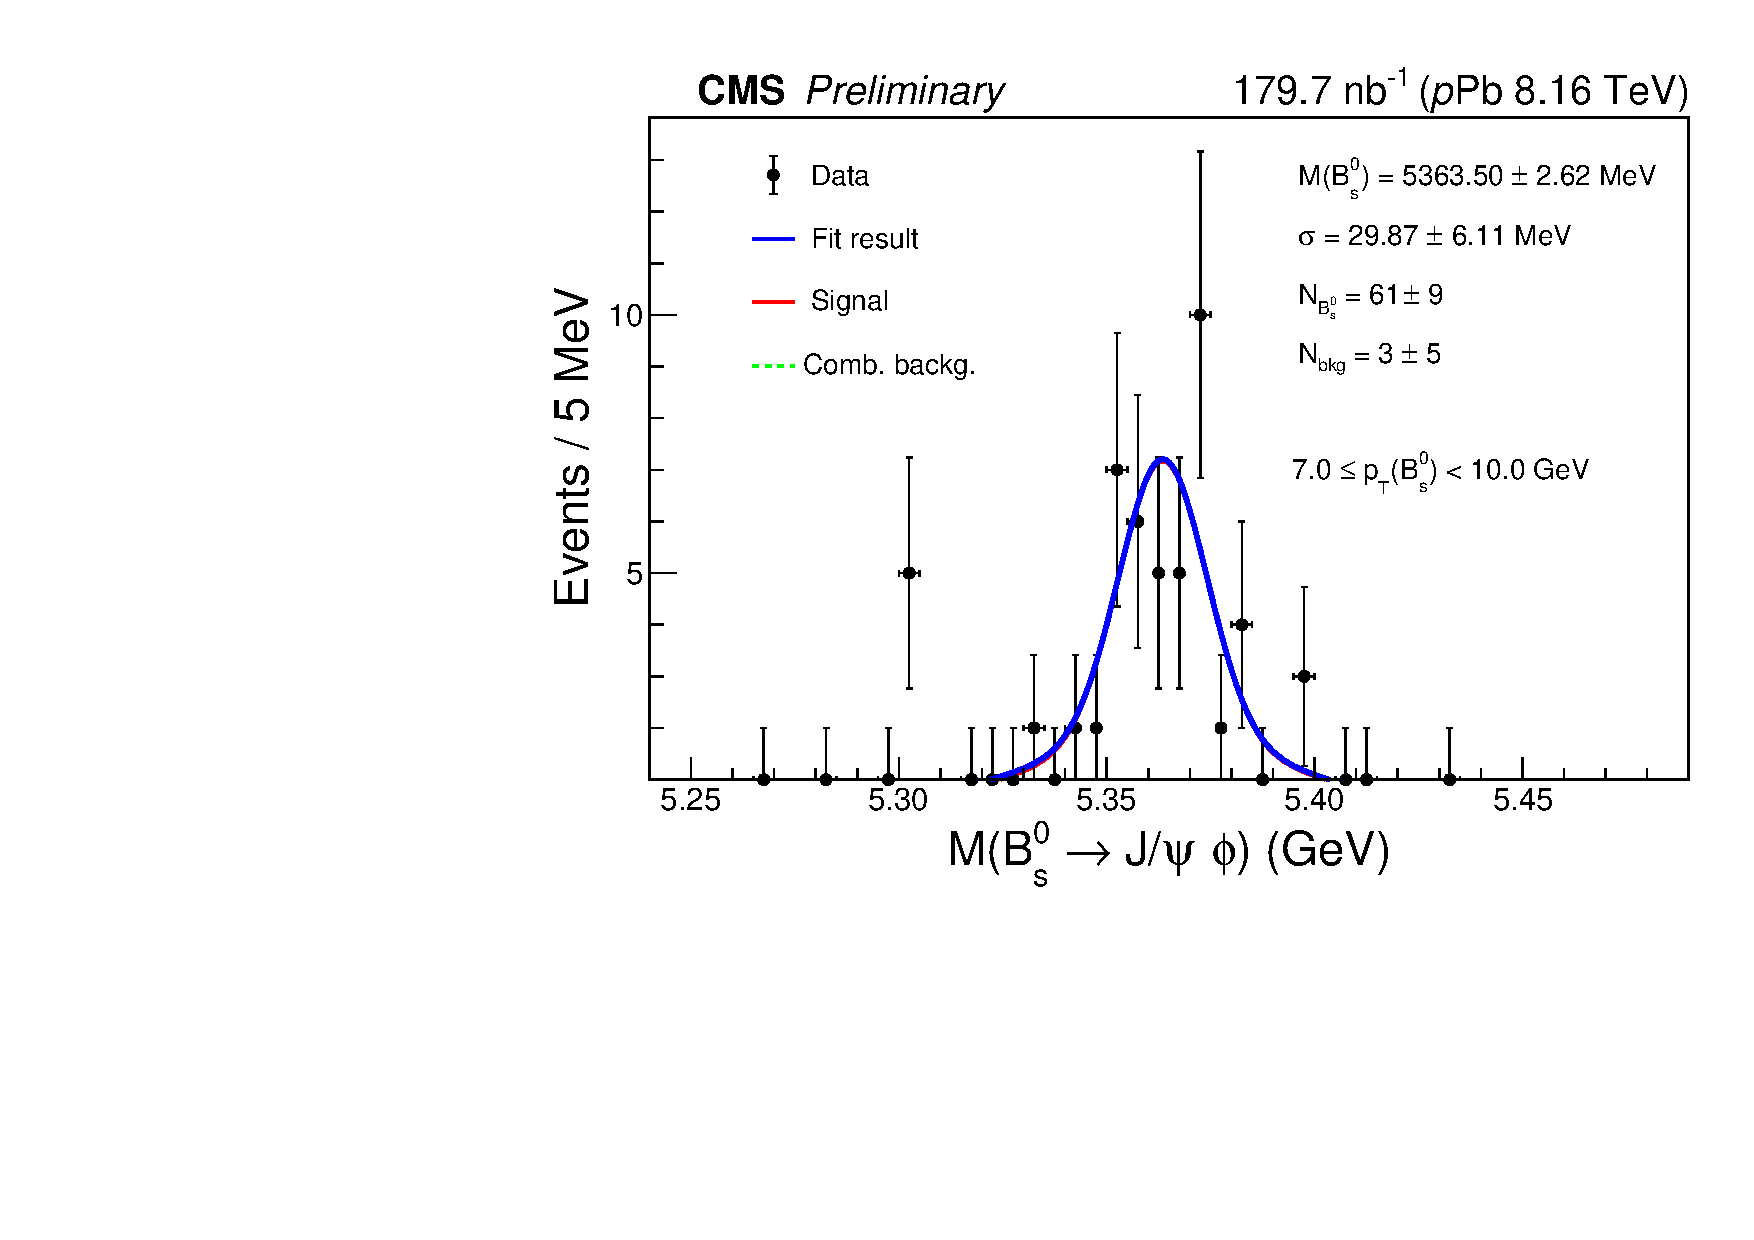
\includegraphics[width=\textwidth]{MainContent/Figs/mass/mass_BsFit_ptbins_syssig_7_10.PDF}
		\caption{}%
	\end{subfigure}
	\hfill
	\begin{subfigure}[b]{0.475\textwidth}
		\centering
		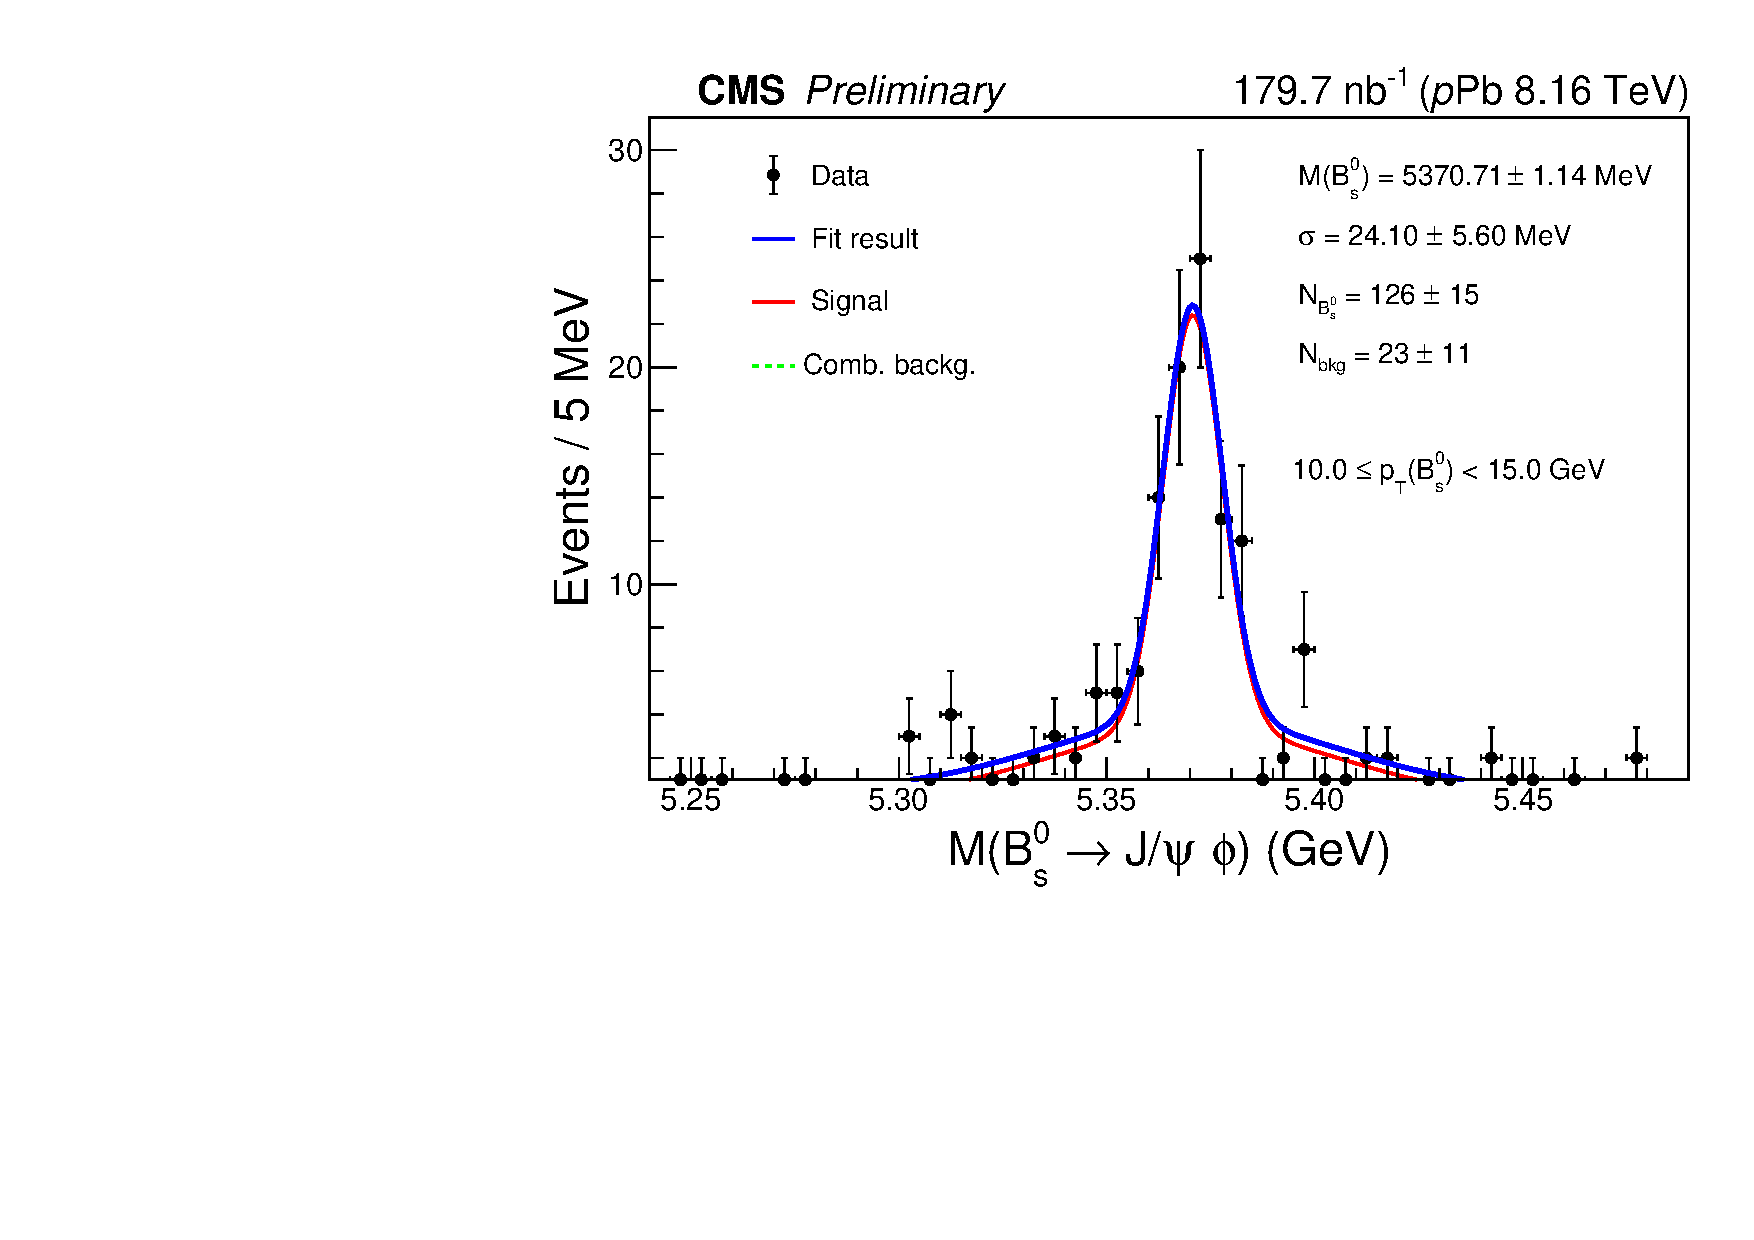
\includegraphics[width=\textwidth]{MainContent/Figs/mass/mass_BsFit_ptbins_syssig_10_15.PDF}
		\caption{}%
	\end{subfigure}
	\vskip\baselineskip
	\begin{subfigure}[b]{0.475\textwidth}
		\centering
		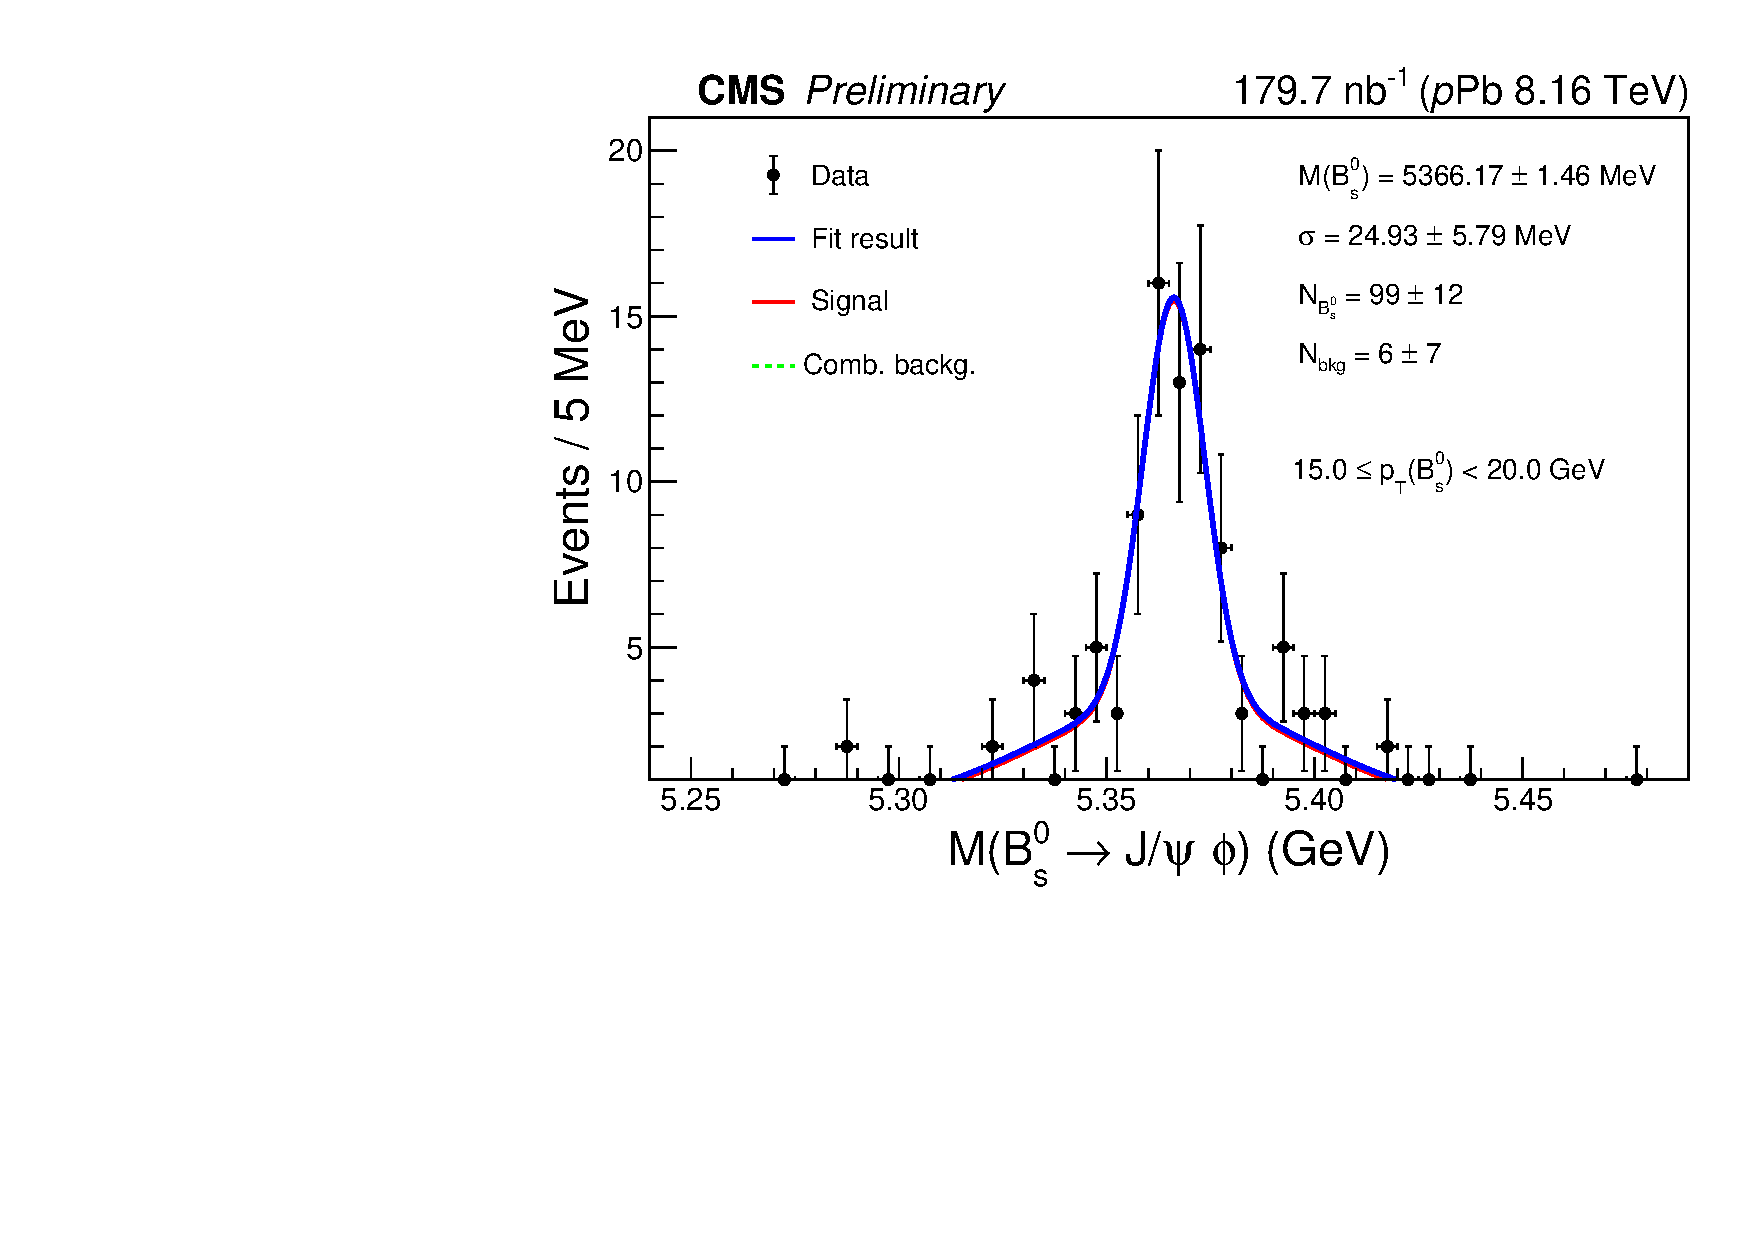
\includegraphics[width=\textwidth]{MainContent/Figs/mass/mass_BsFit_ptbins_syssig_15_20.PDF}
		\caption{}
	\end{subfigure}
	\hfill
	\begin{subfigure}[b]{0.475\textwidth}
		\centering
		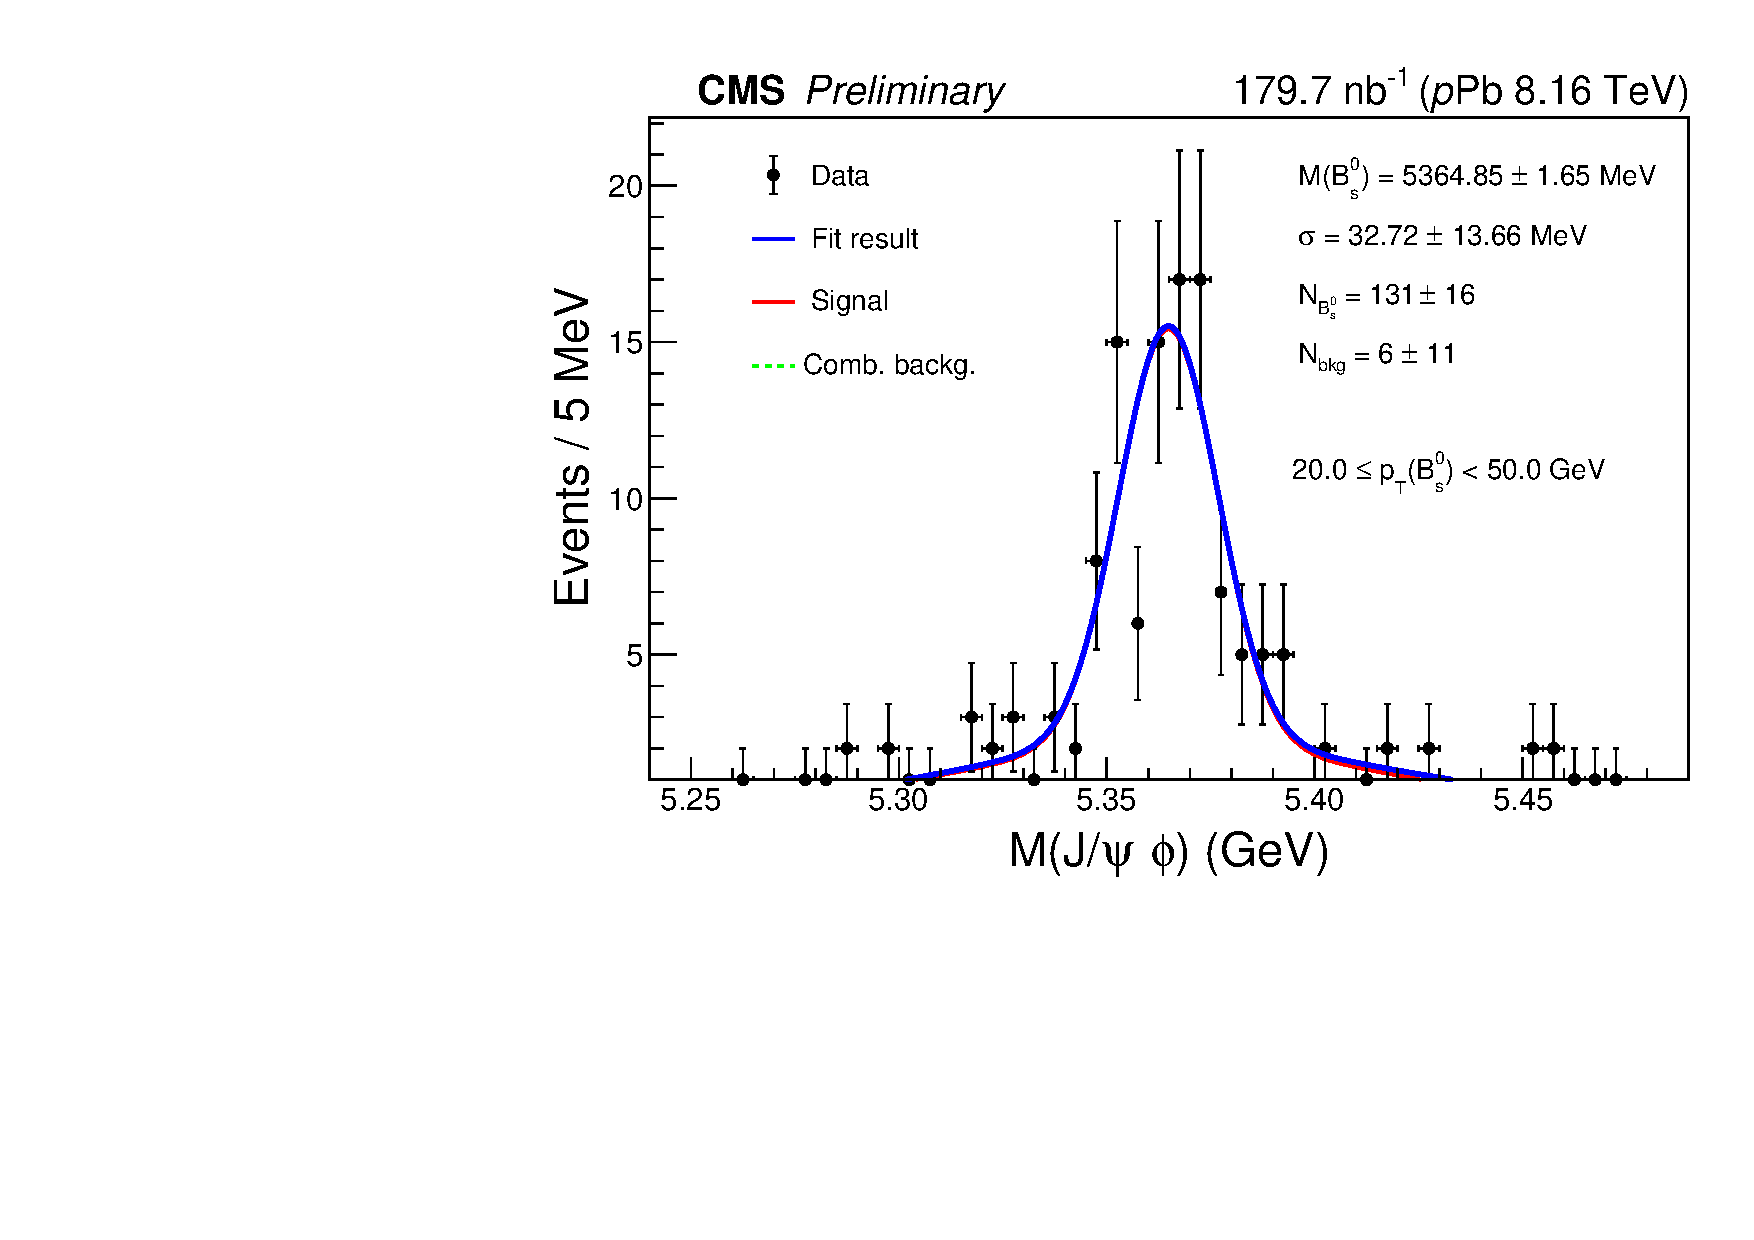
\includegraphics[width=\textwidth]{MainContent/Figs/mass/mass_BsFit_ptbins_syssig_20_50.PDF}
		\caption{}%
	\end{subfigure}
	\caption{Invariant mass spectra for $B^0_s$ meson reconstructed from the combined system $J/\psi \phi$ and considering a systematic model for signal. Four intervals for the transverse momentum $p_T(B^0_s)$ have been considered.}
	\label{fig:mass_ptbins_syssig}
	%%%%%%%%%%%%%%%%%%%%%%%%%%%%%%%%%%%%second row
	
\end{figure}

\begin{figure}[htp!]
	\centering
	\centering
	\begin{subfigure}[b]{0.475\textwidth}
		\centering
		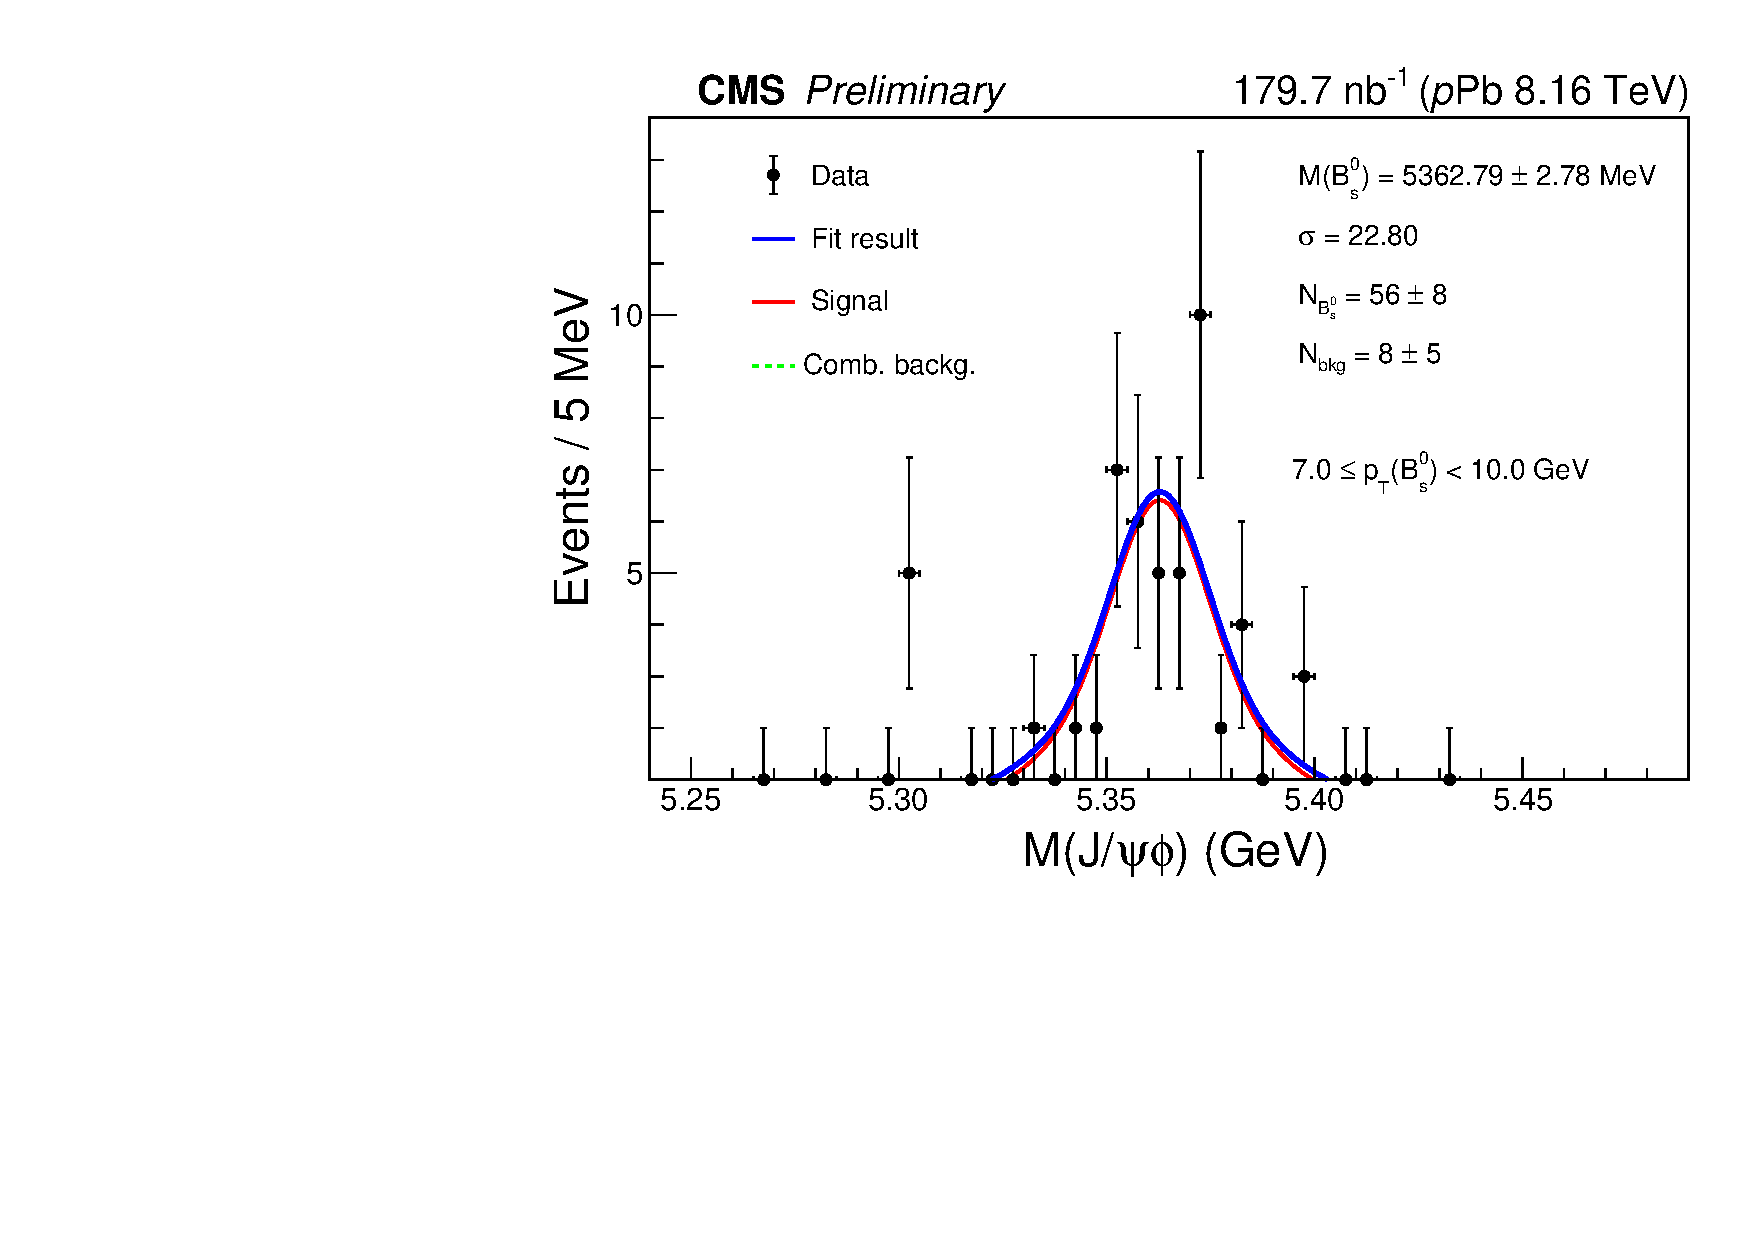
\includegraphics[width=\textwidth]{MainContent/Figs/mass/mass_BsFit_ptbins_sysbkg_7_10.PDF}
		\caption{}%
	\end{subfigure}
	\hfill
	\begin{subfigure}[b]{0.475\textwidth}
		\centering
		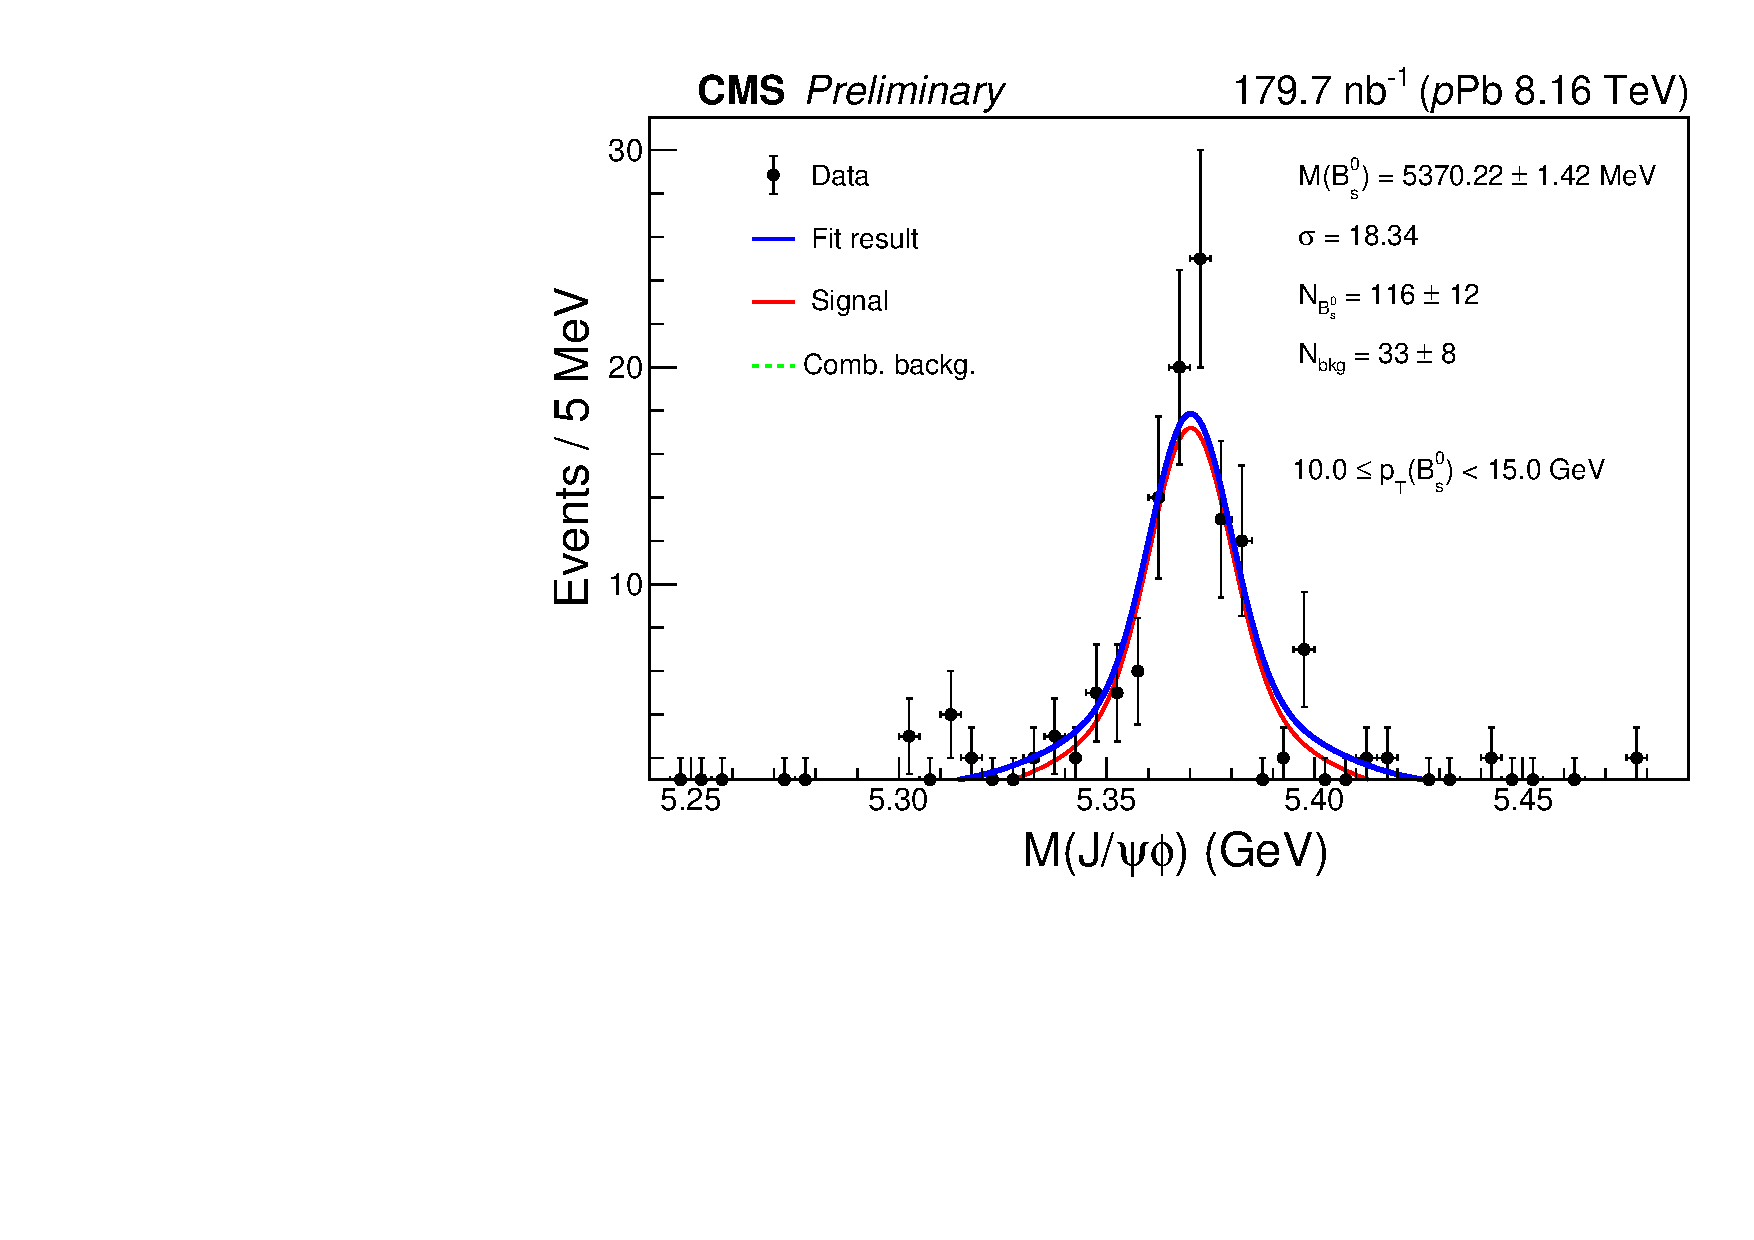
\includegraphics[width=\textwidth]{MainContent/Figs/mass/mass_BsFit_ptbins_sysbkg_10_15.PDF}
		\caption{}%
	\end{subfigure}
	\vskip\baselineskip
	\begin{subfigure}[b]{0.475\textwidth}
		\centering
		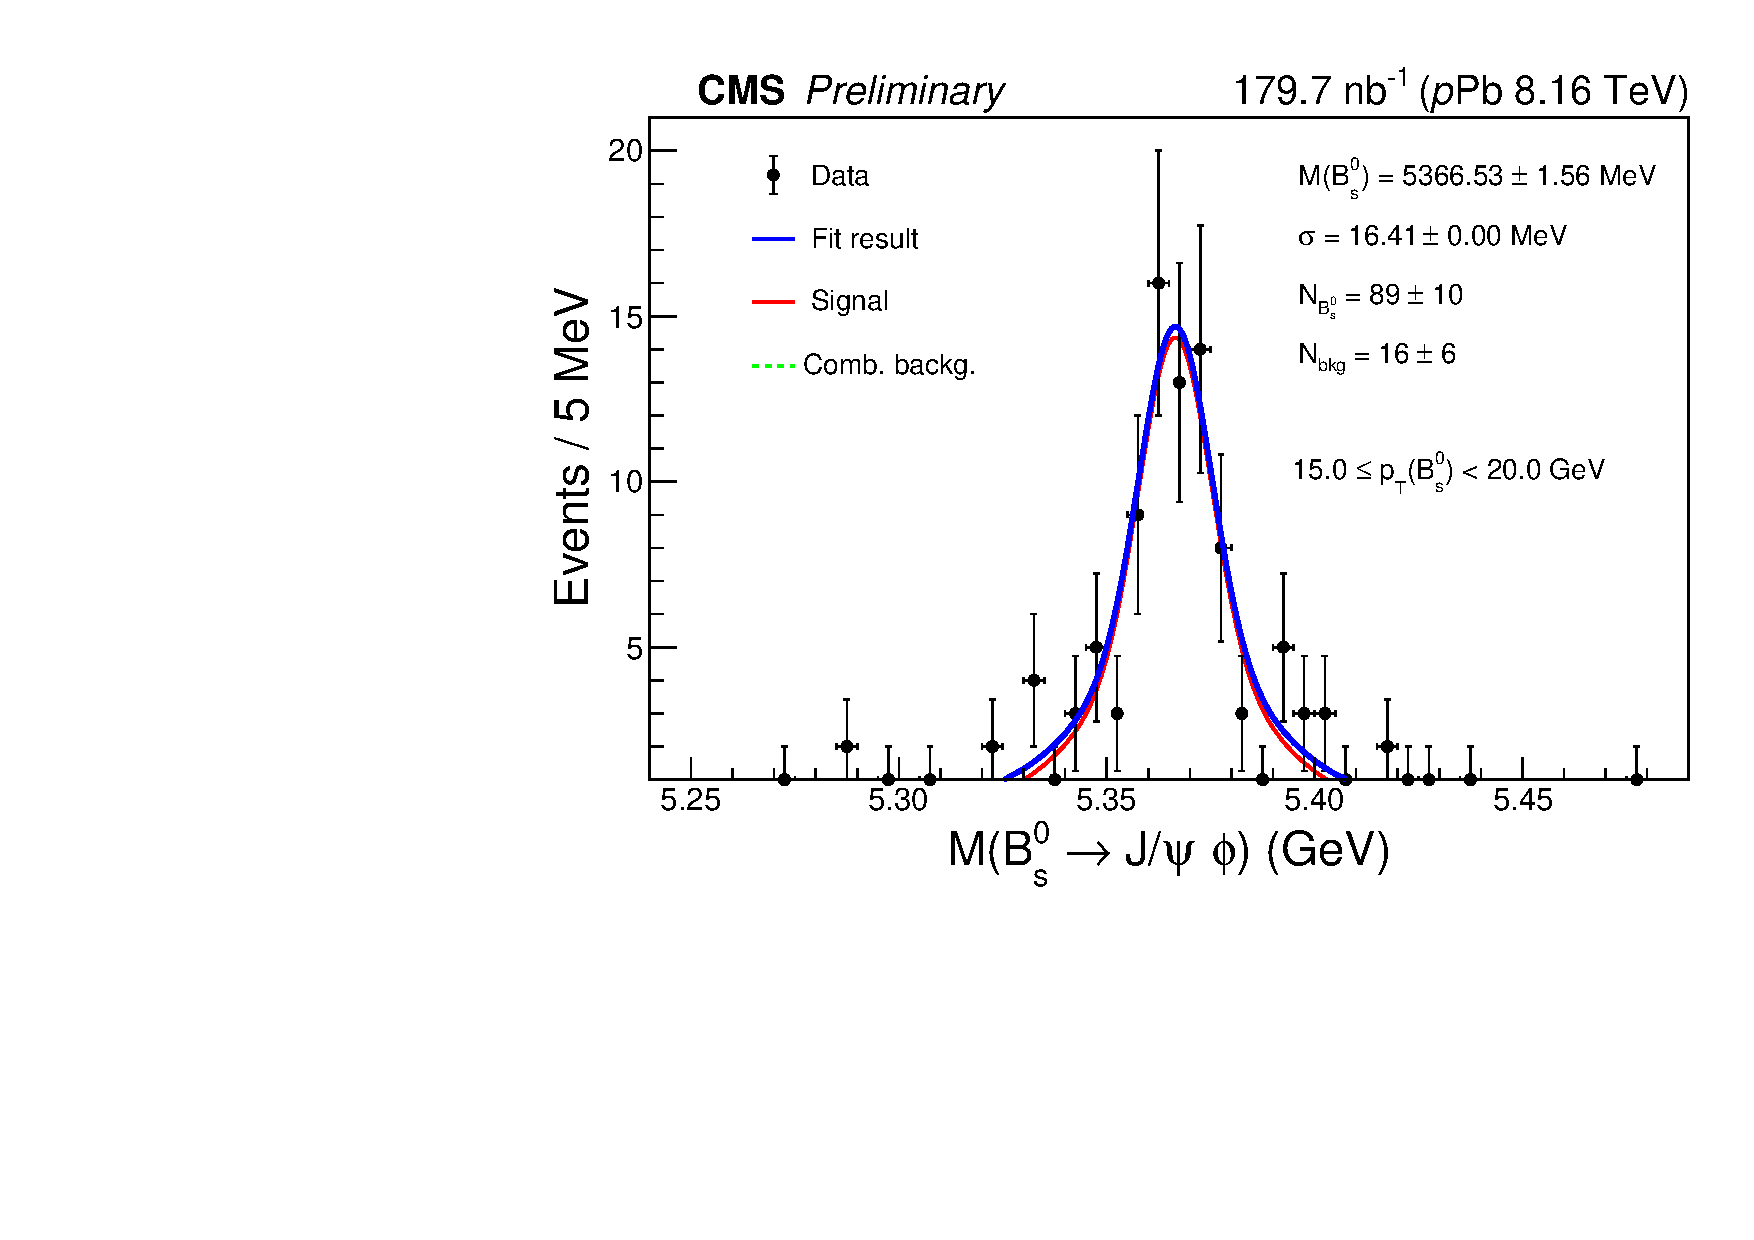
\includegraphics[width=\textwidth]{MainContent/Figs/mass/mass_BsFit_ptbins_sysbkg_15_20.PDF}
		\caption{}
	\end{subfigure}
	\hfill
	\begin{subfigure}[b]{0.475\textwidth}
		\centering
		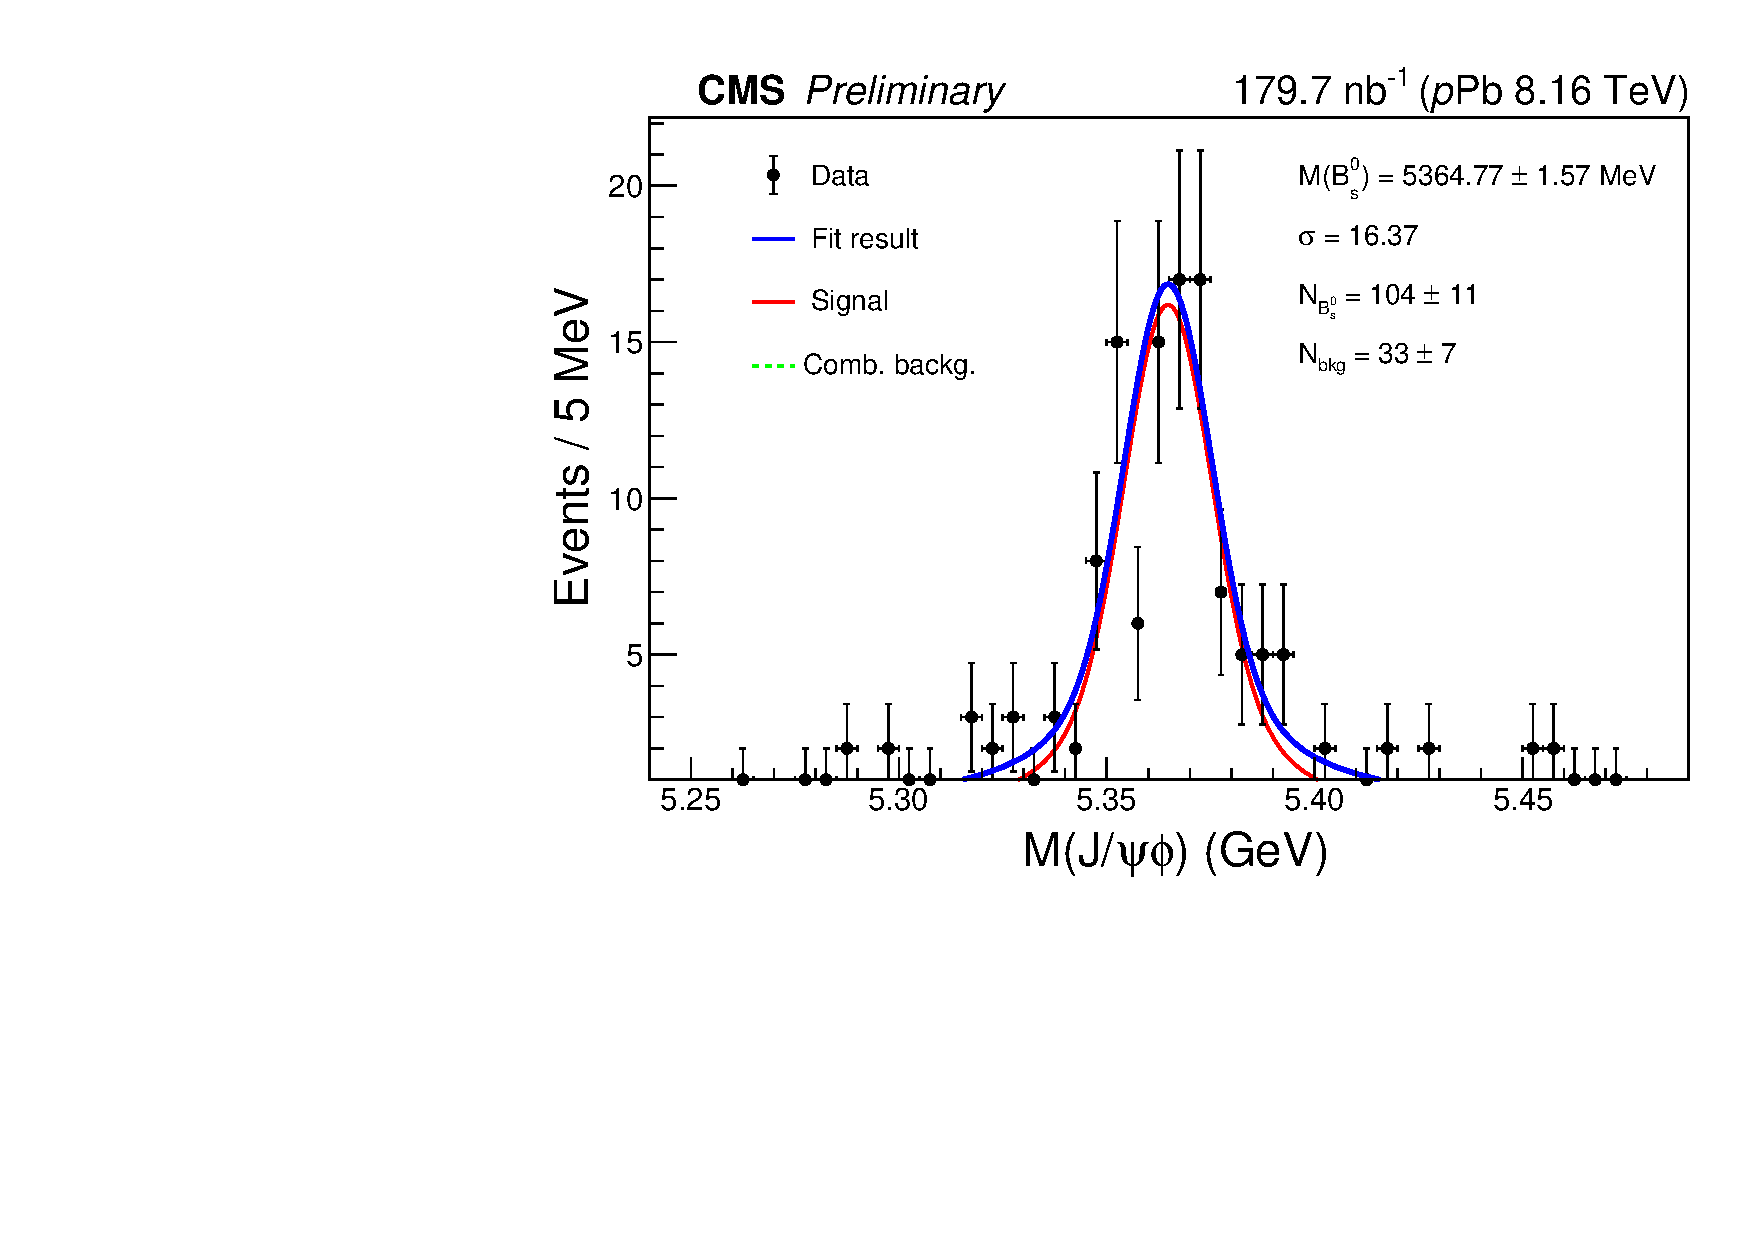
\includegraphics[width=\textwidth]{MainContent/Figs/mass/mass_BsFit_ptbins_sysbkg_20_50.PDF}
		\caption{}%
	\end{subfigure}
	\caption{Invariant mass spectra for $B^0_s$ meson reconstructed from the combined system $J/\psi \phi$ and considering a systematic model for background. Four intervals for the transverse momentum $p_T(B^0_s)$ have been considered.}
	\label{fig:mass_ptbins_sysbkg}
	%%%%%%%%%%%%%%%%%%%%%%%%%%%%%%%%%%%%second row
	
\end{figure}



\begin{figure*}
	\centering
	\begin{subfigure}[b]{0.7\textwidth}
		\centering
		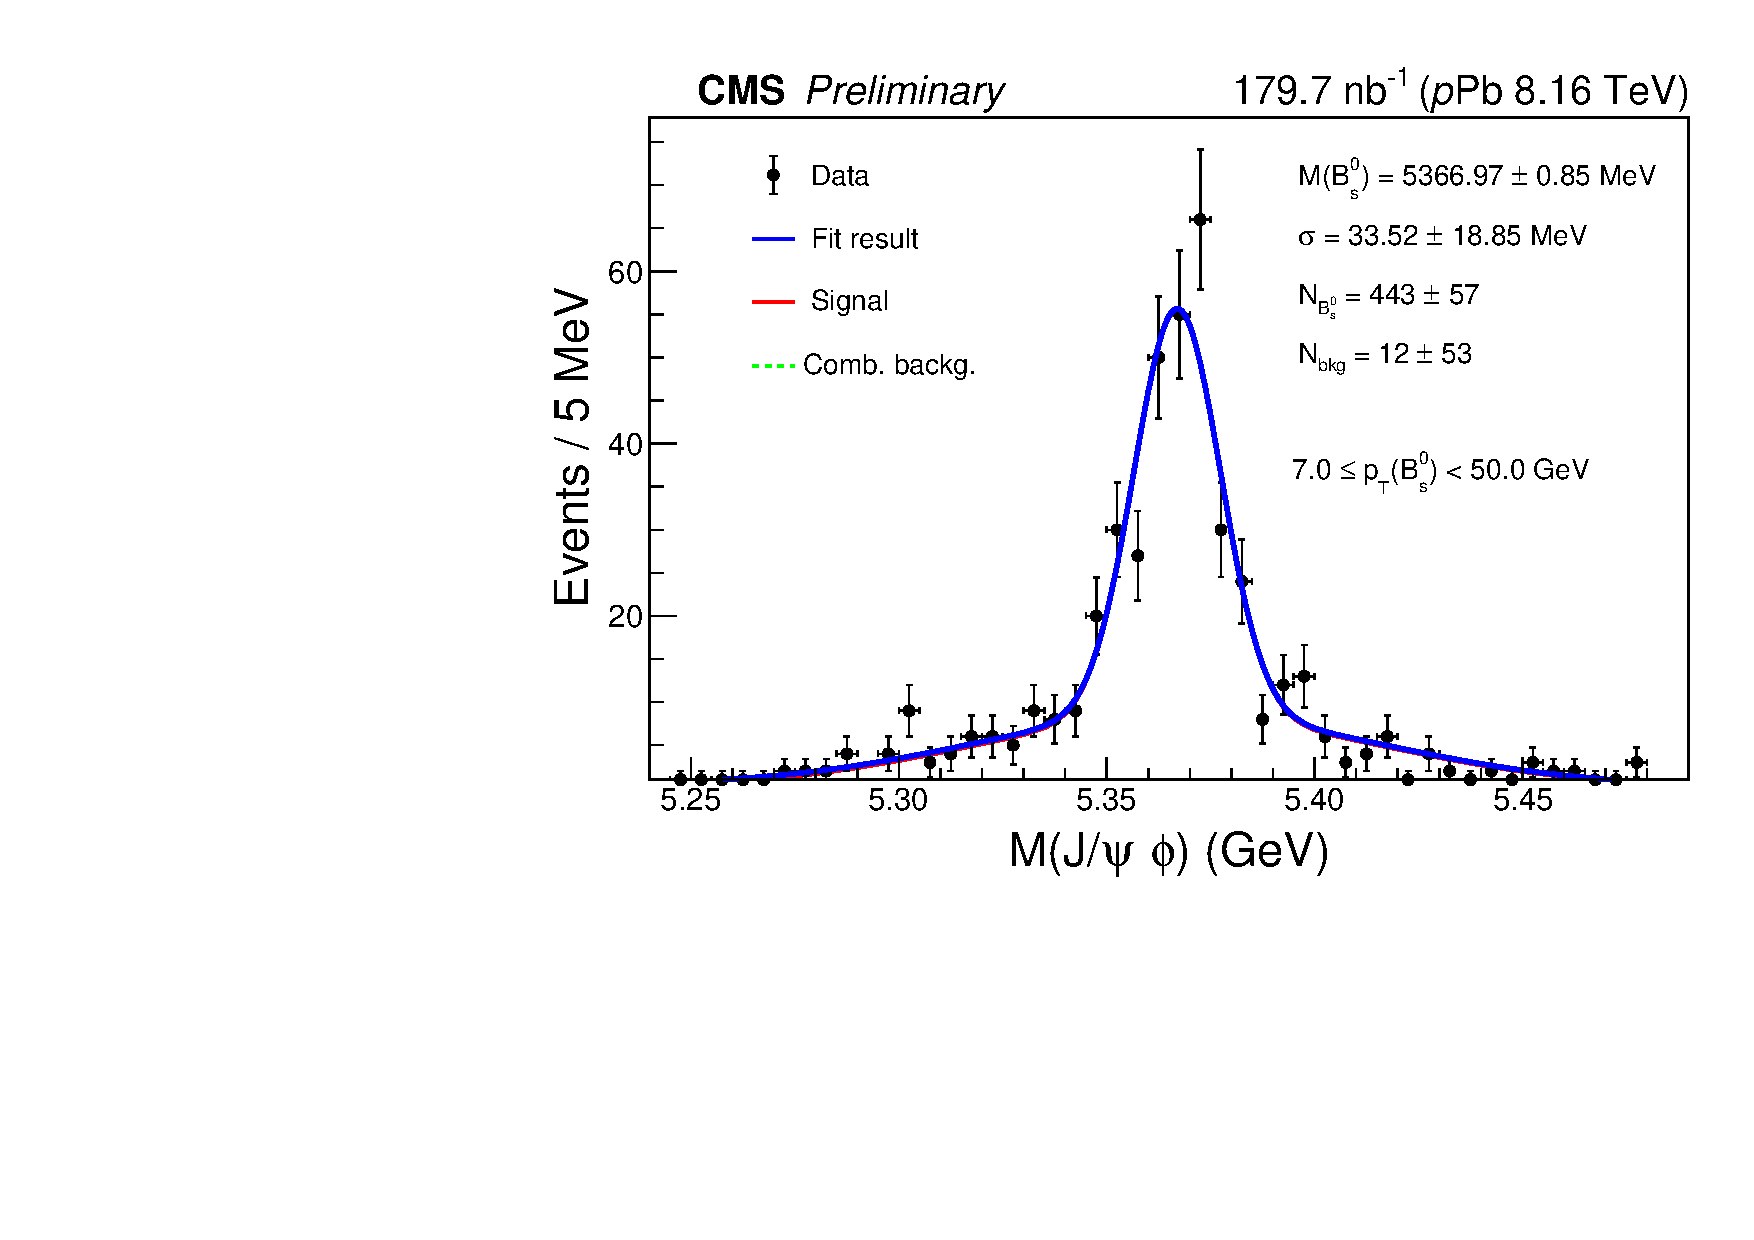
\includegraphics[width=\textwidth]{MainContent/Figs/mass/mass_BsFit_ptbins_syssig_7_50.PDF}
		\caption{}%
	\end{subfigure}
	\vskip\baselineskip
	\begin{subfigure}[b]{0.7\textwidth}
		\centering
		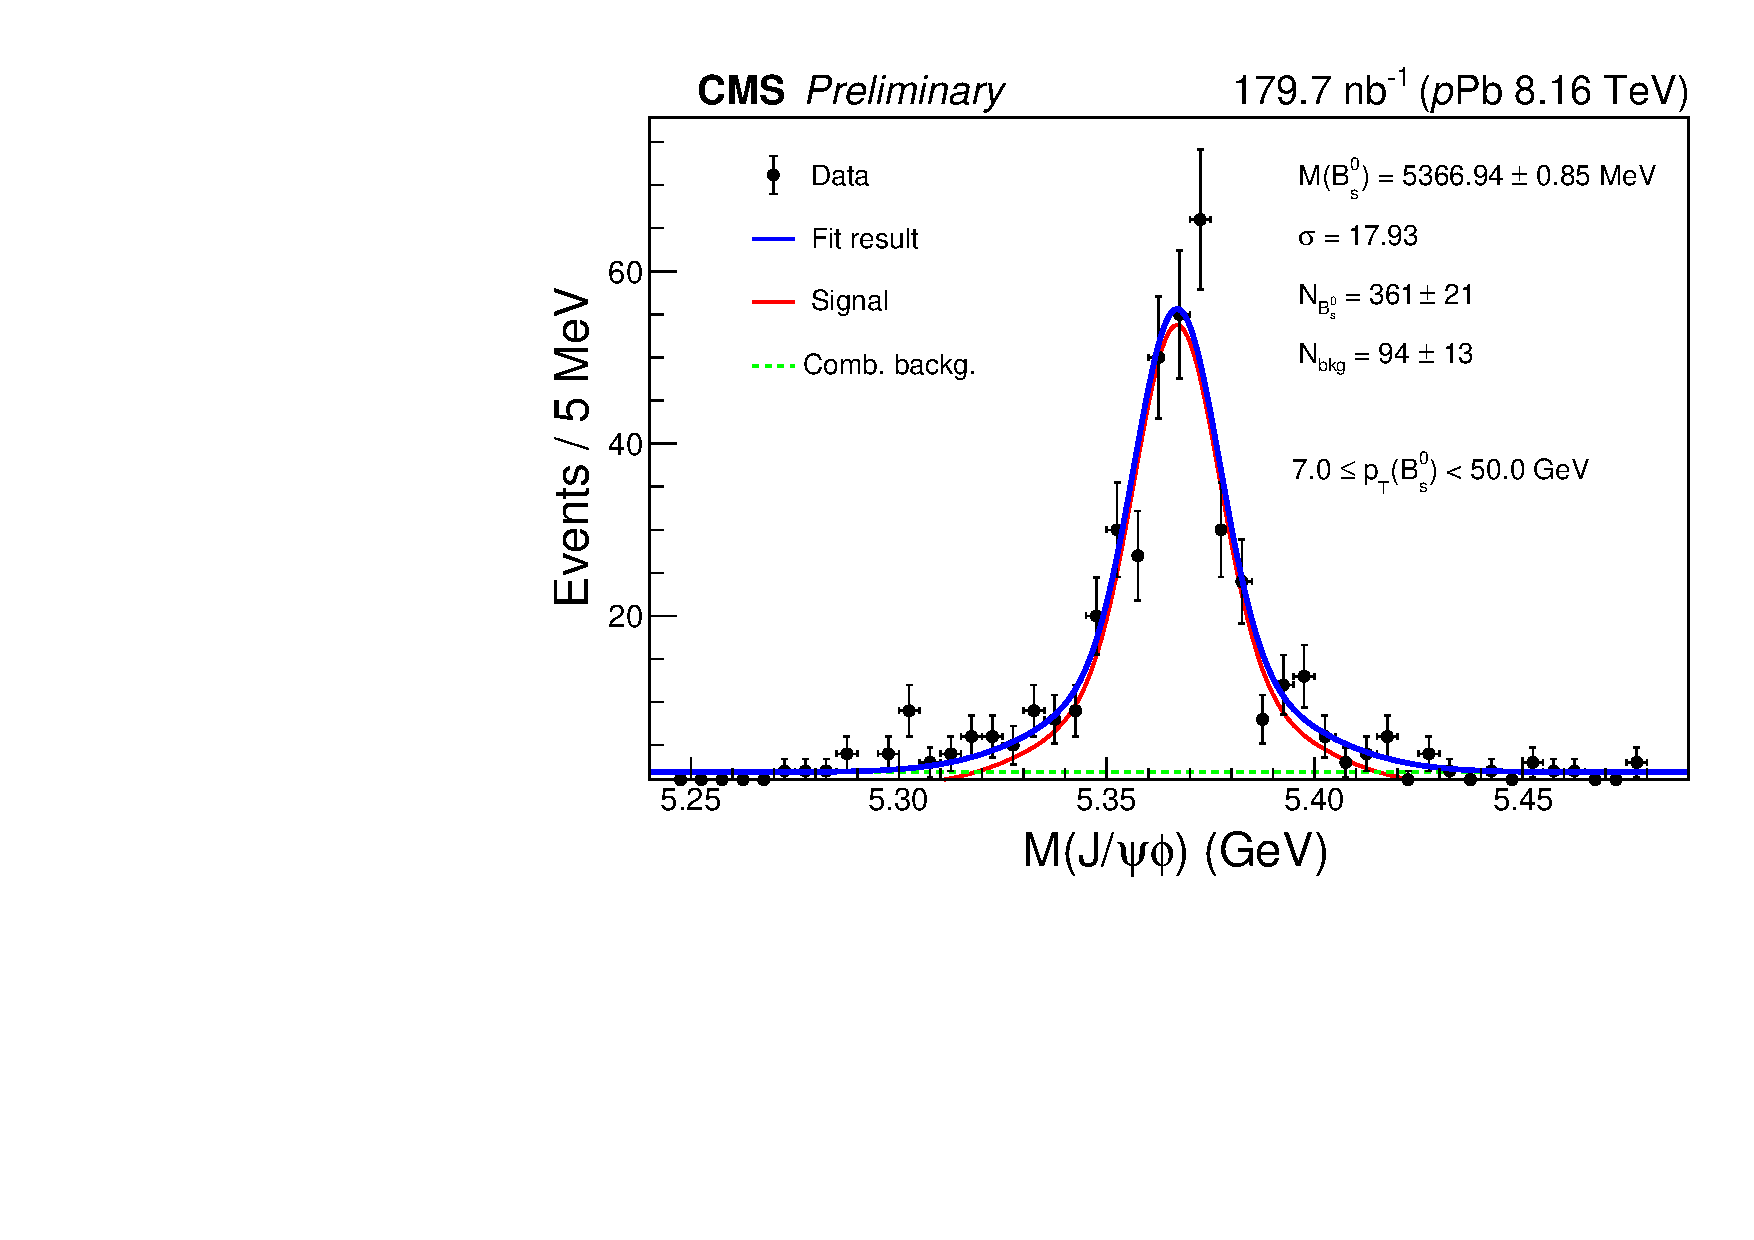
\includegraphics[width=\textwidth]{MainContent/Figs/mass/mass_BsFit_ptbins_sysbkg_7_50.PDF}
		\caption{}%
	\end{subfigure}
	\caption{Invariant mass spectra for the $B^0_s$ meson reconstructed from the combined system $J/\psi \phi$. a) corresponds to the systematic model for signal b) for background}
	\label{fig:mass_ptbins_sys}
\end{figure*}

\begin{figure}[htp!]
	\centering
	\centering
	\begin{subfigure}[b]{0.475\textwidth}
		\centering
		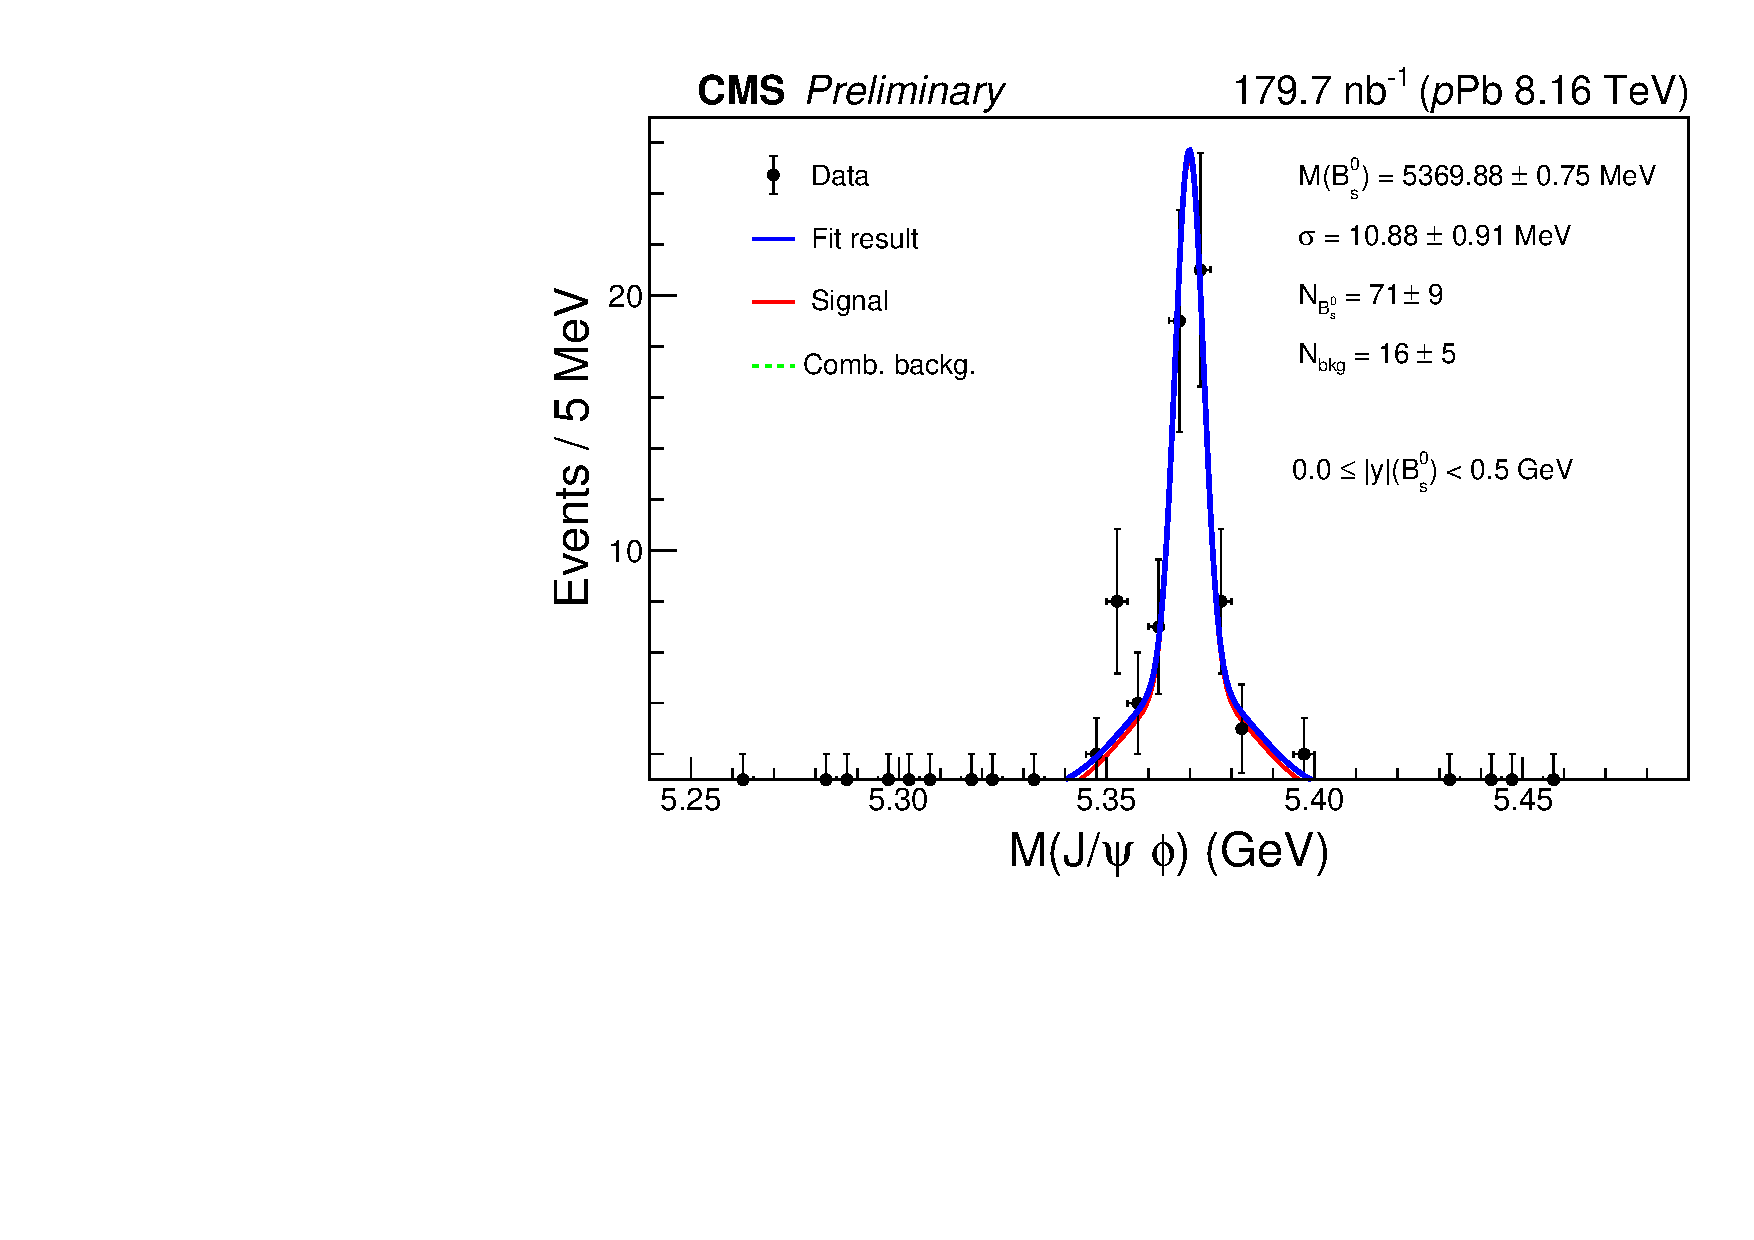
\includegraphics[width=\textwidth]{MainContent/Figs/mass/mass_BsFit_ybins_syssig_0.0_0.5.PDF}
		\caption{}%
	\end{subfigure}
	\hfill
	\begin{subfigure}[b]{0.475\textwidth}
		\centering
		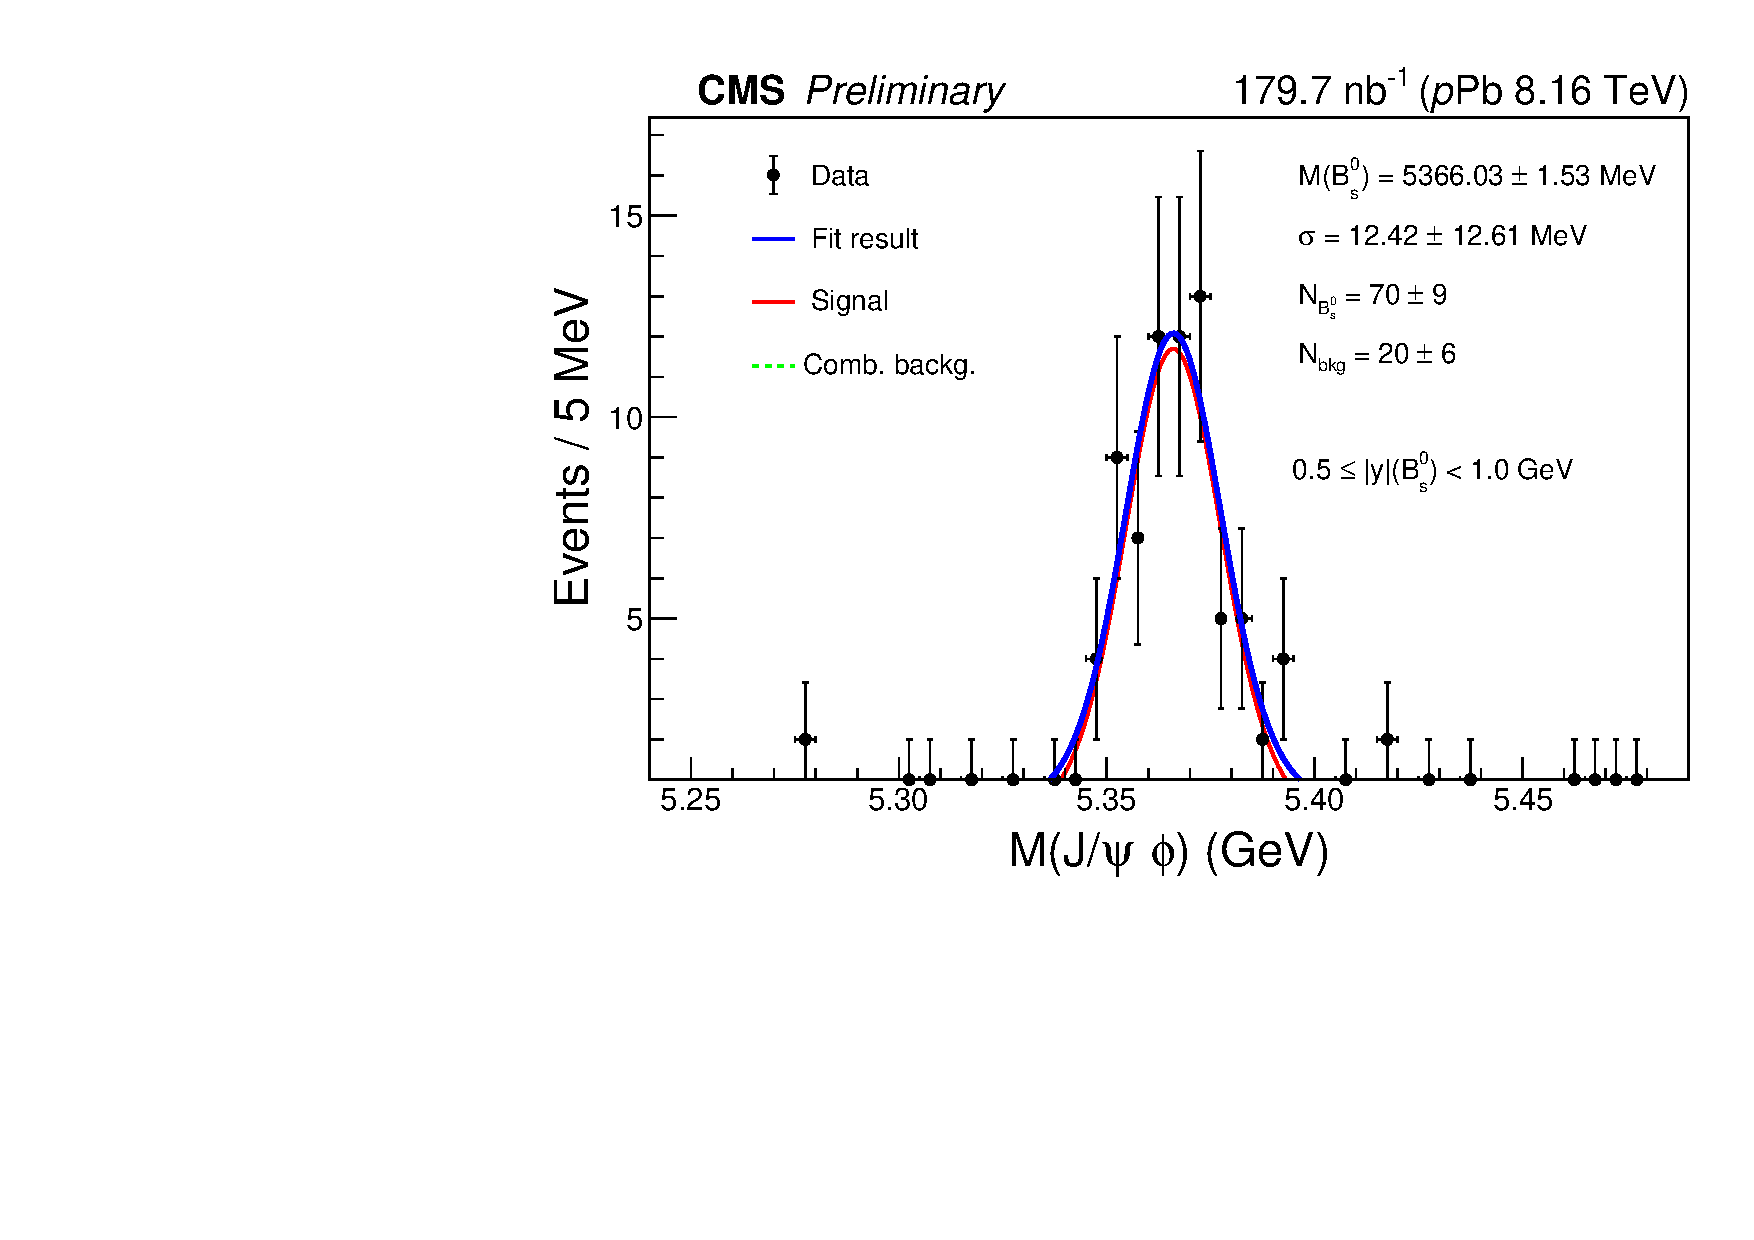
\includegraphics[width=\textwidth]{MainContent/Figs/mass/mass_BsFit_ybins_syssig_0.5_1.0.PDF}
		\caption{}%
		
	\end{subfigure}
	\vskip\baselineskip
	\begin{subfigure}[b]{0.475\textwidth}
		\centering
		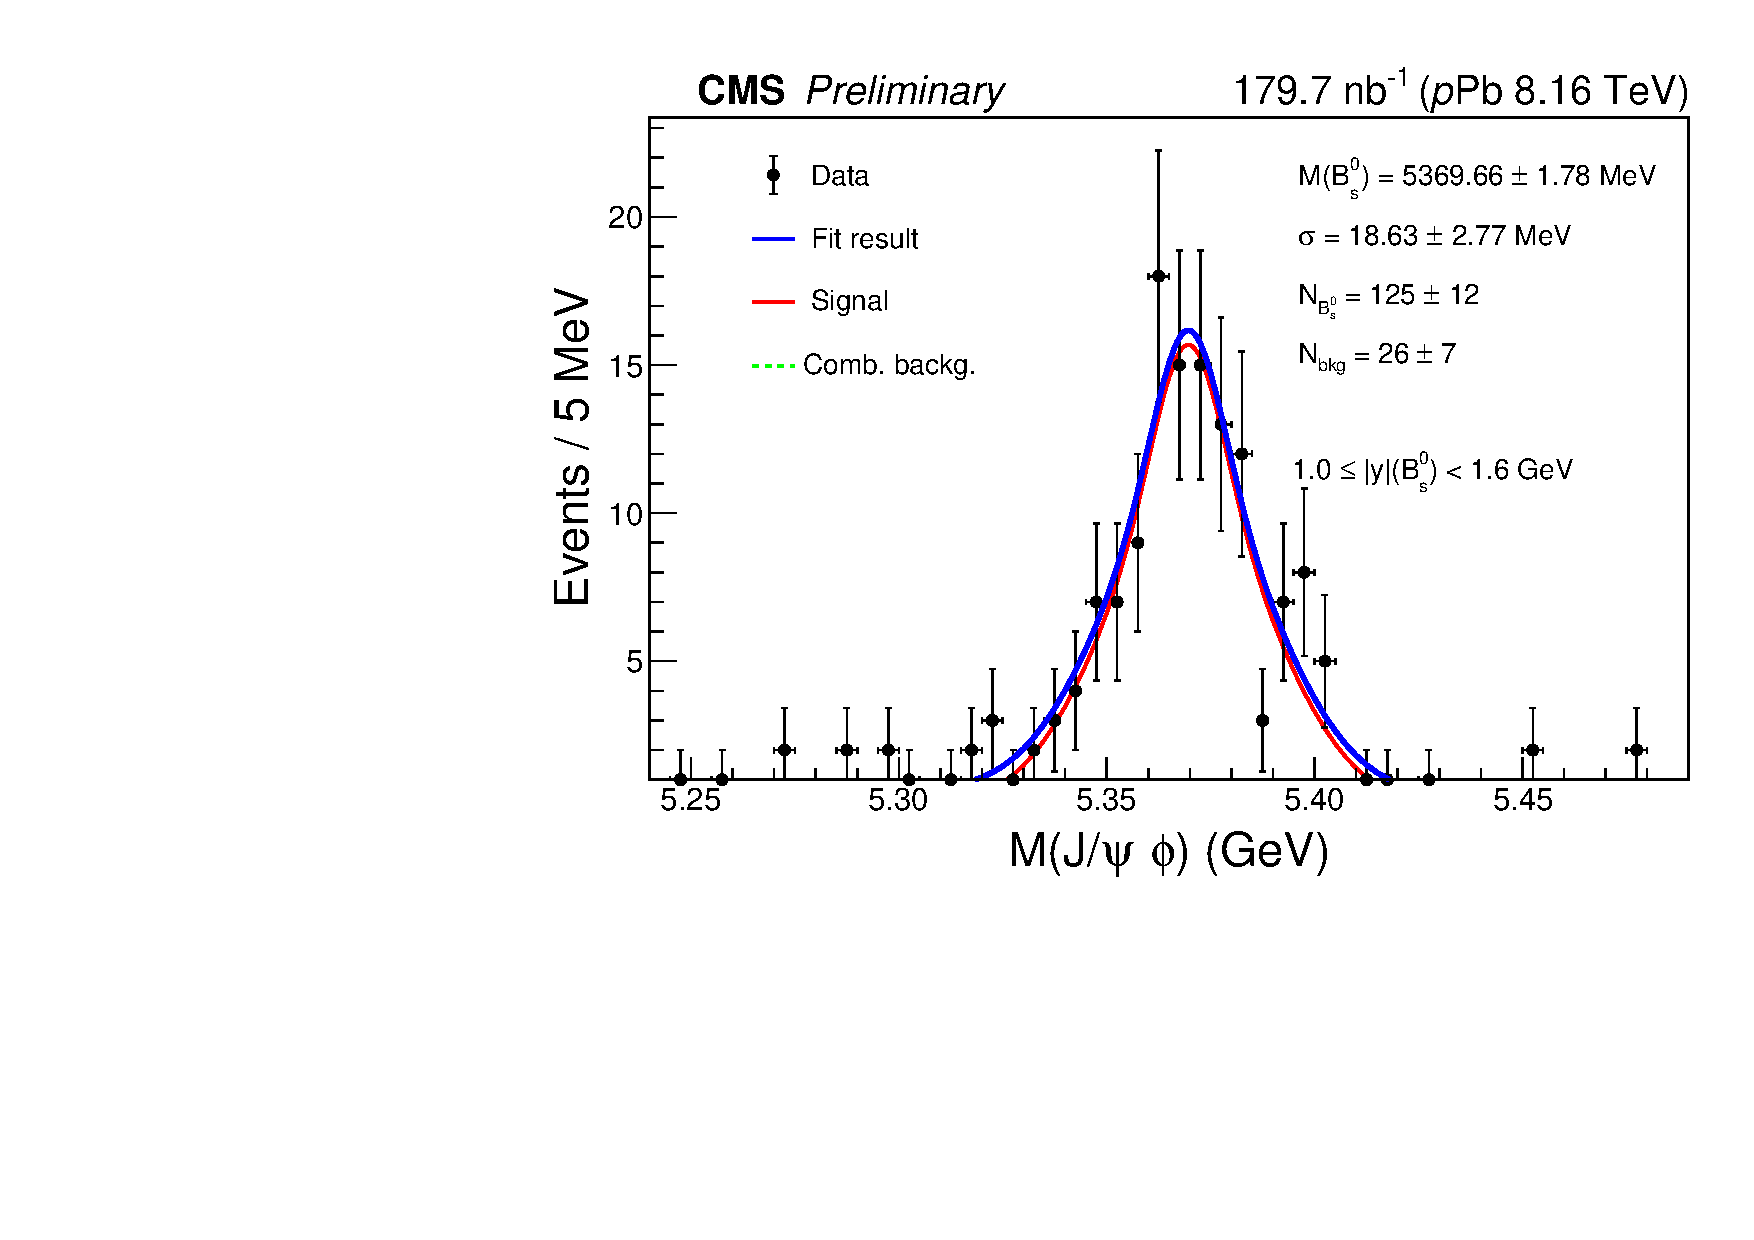
\includegraphics[width=\textwidth]{MainContent/Figs/mass/mass_BsFit_ybins_syssig_1.0_1.6.PDF}
		\caption{}
	\end{subfigure}
	\hfill
	\begin{subfigure}[b]{0.475\textwidth}
		\centering
		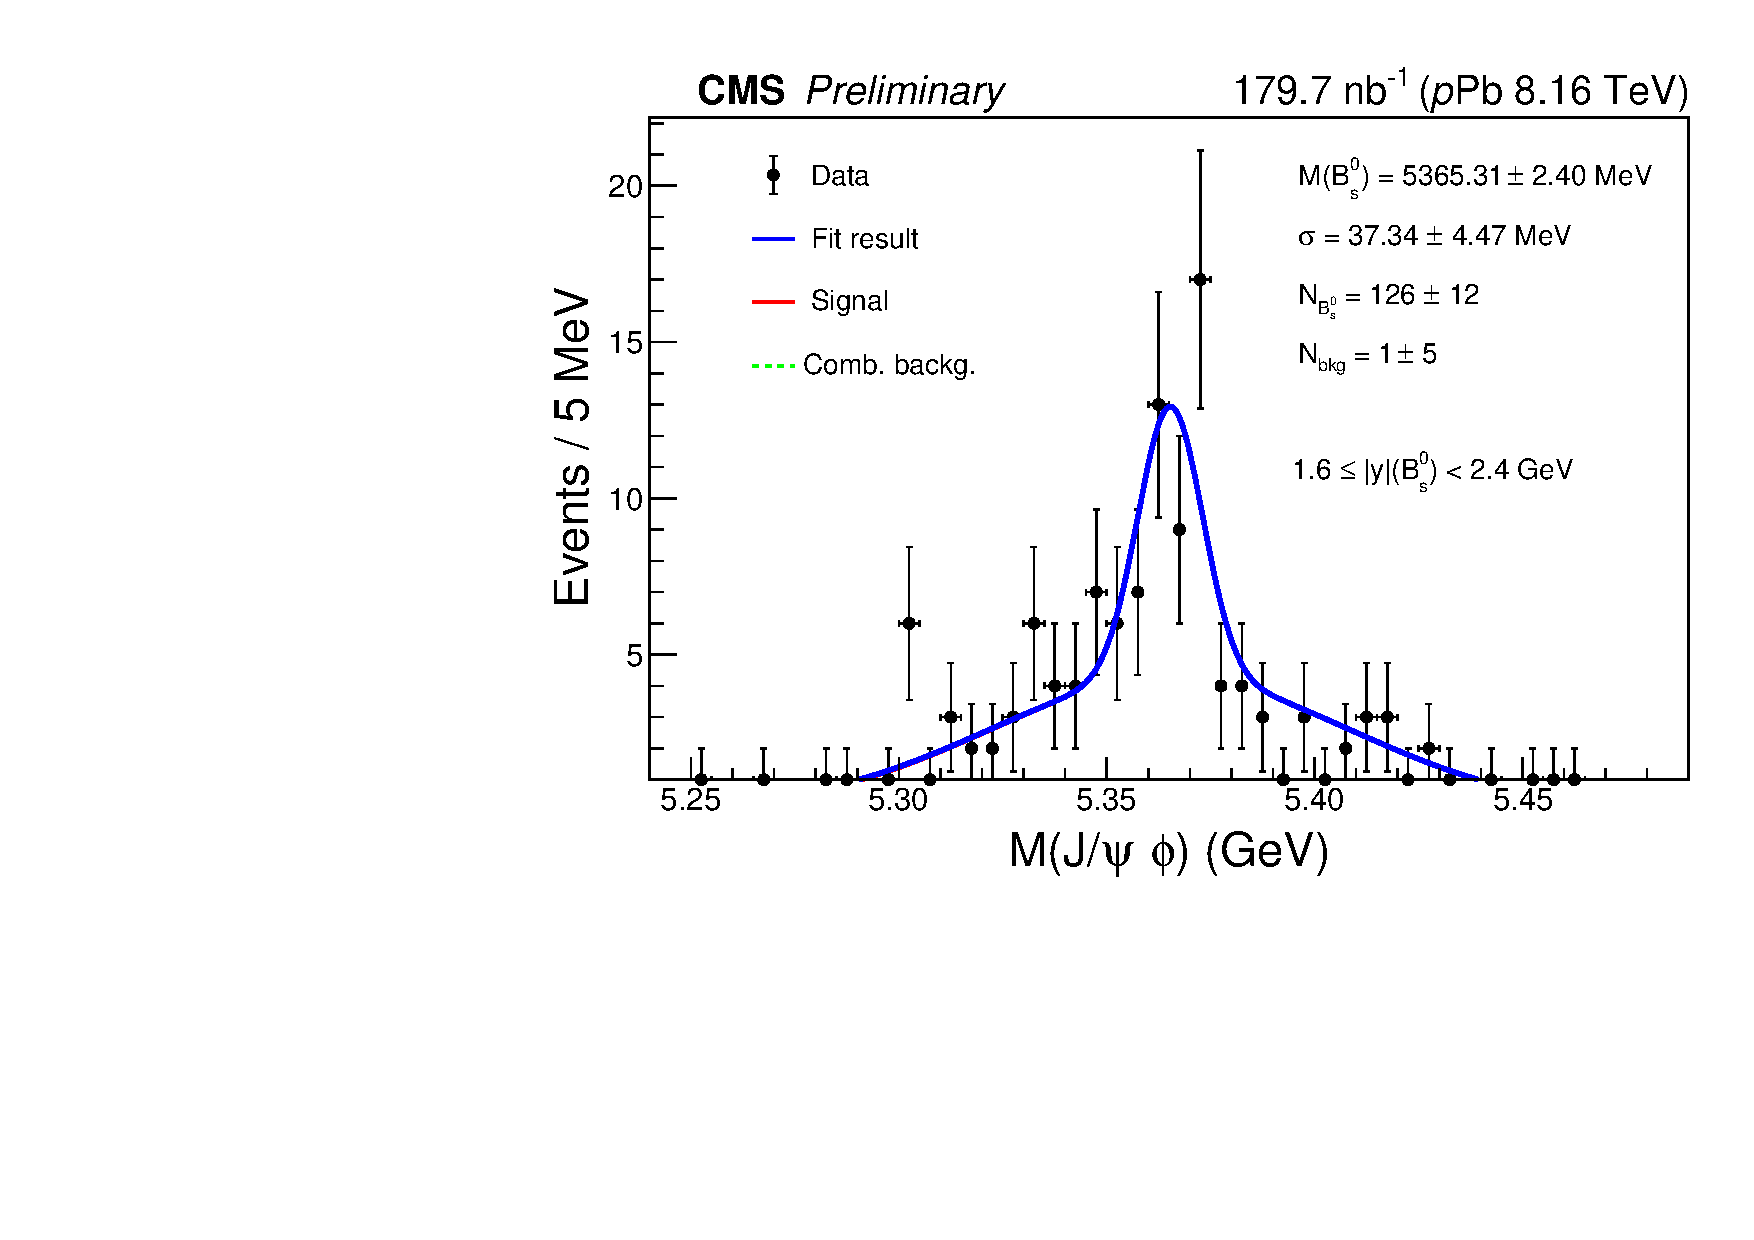
\includegraphics[width=\textwidth]{MainContent/Figs/mass/mass_BsFit_ybins_syssig_1.6_2.4.PDF}
		\caption{}%
	\end{subfigure}
	\caption{Invariant mass spectra for $B^0_s$ meson reconstructed from the combined system $J/\psi \phi$ and considering a systematic model for signal. Four intervals for the rapidity $|y|(B^0_s)$ have been considered.}
	\label{fig:mass_ybins_syssig}
	%%%%%%%%%%%%%%%%%%%%%%%%%%%%%%%%%%%%second row
	
\end{figure}


\begin{figure}[htp!]
	\centering
	\centering
	\begin{subfigure}[b]{0.475\textwidth}
		\centering
		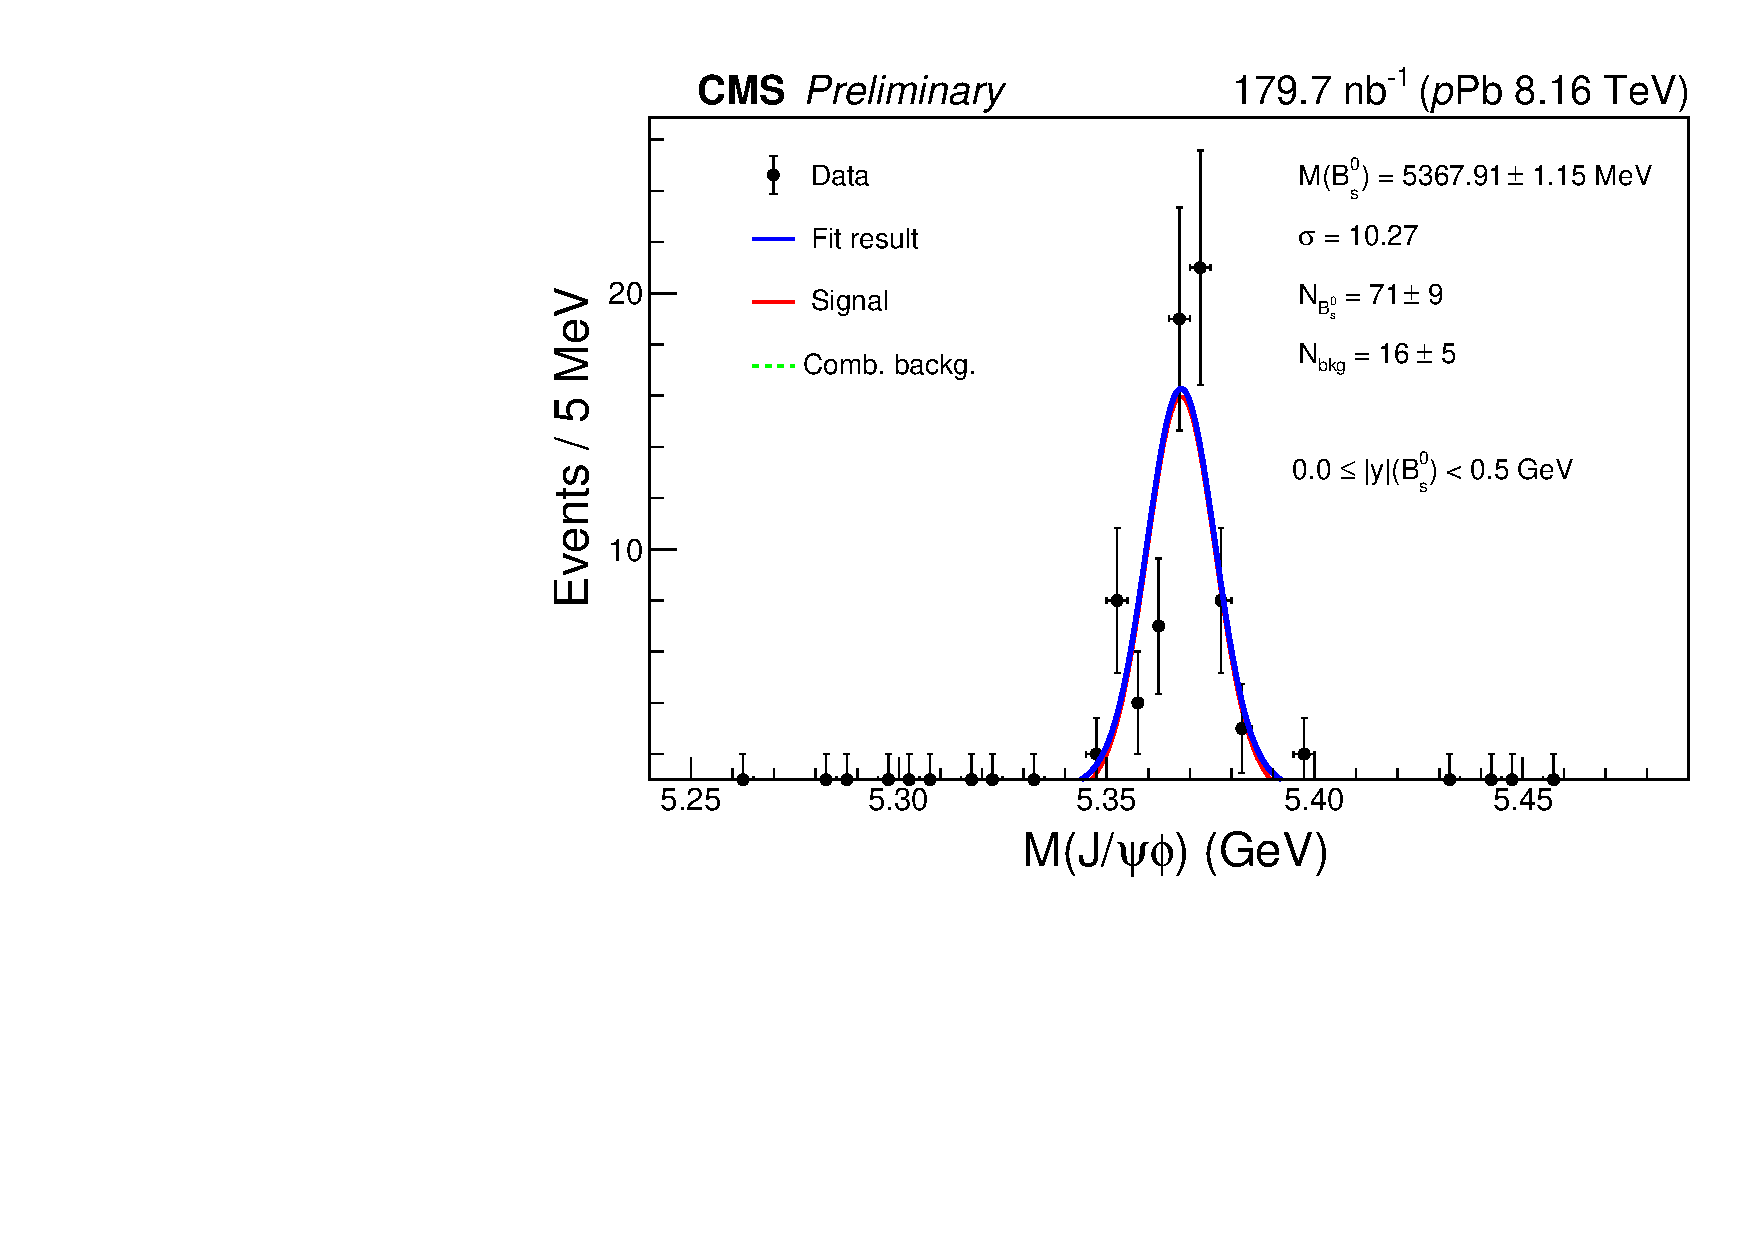
\includegraphics[width=\textwidth]{MainContent/Figs/mass/mass_BsFit_ybins_sysbkg_0.0_0.5.PDF}
		\caption{}%
	\end{subfigure}
	\hfill
	\begin{subfigure}[b]{0.475\textwidth}
		\centering
		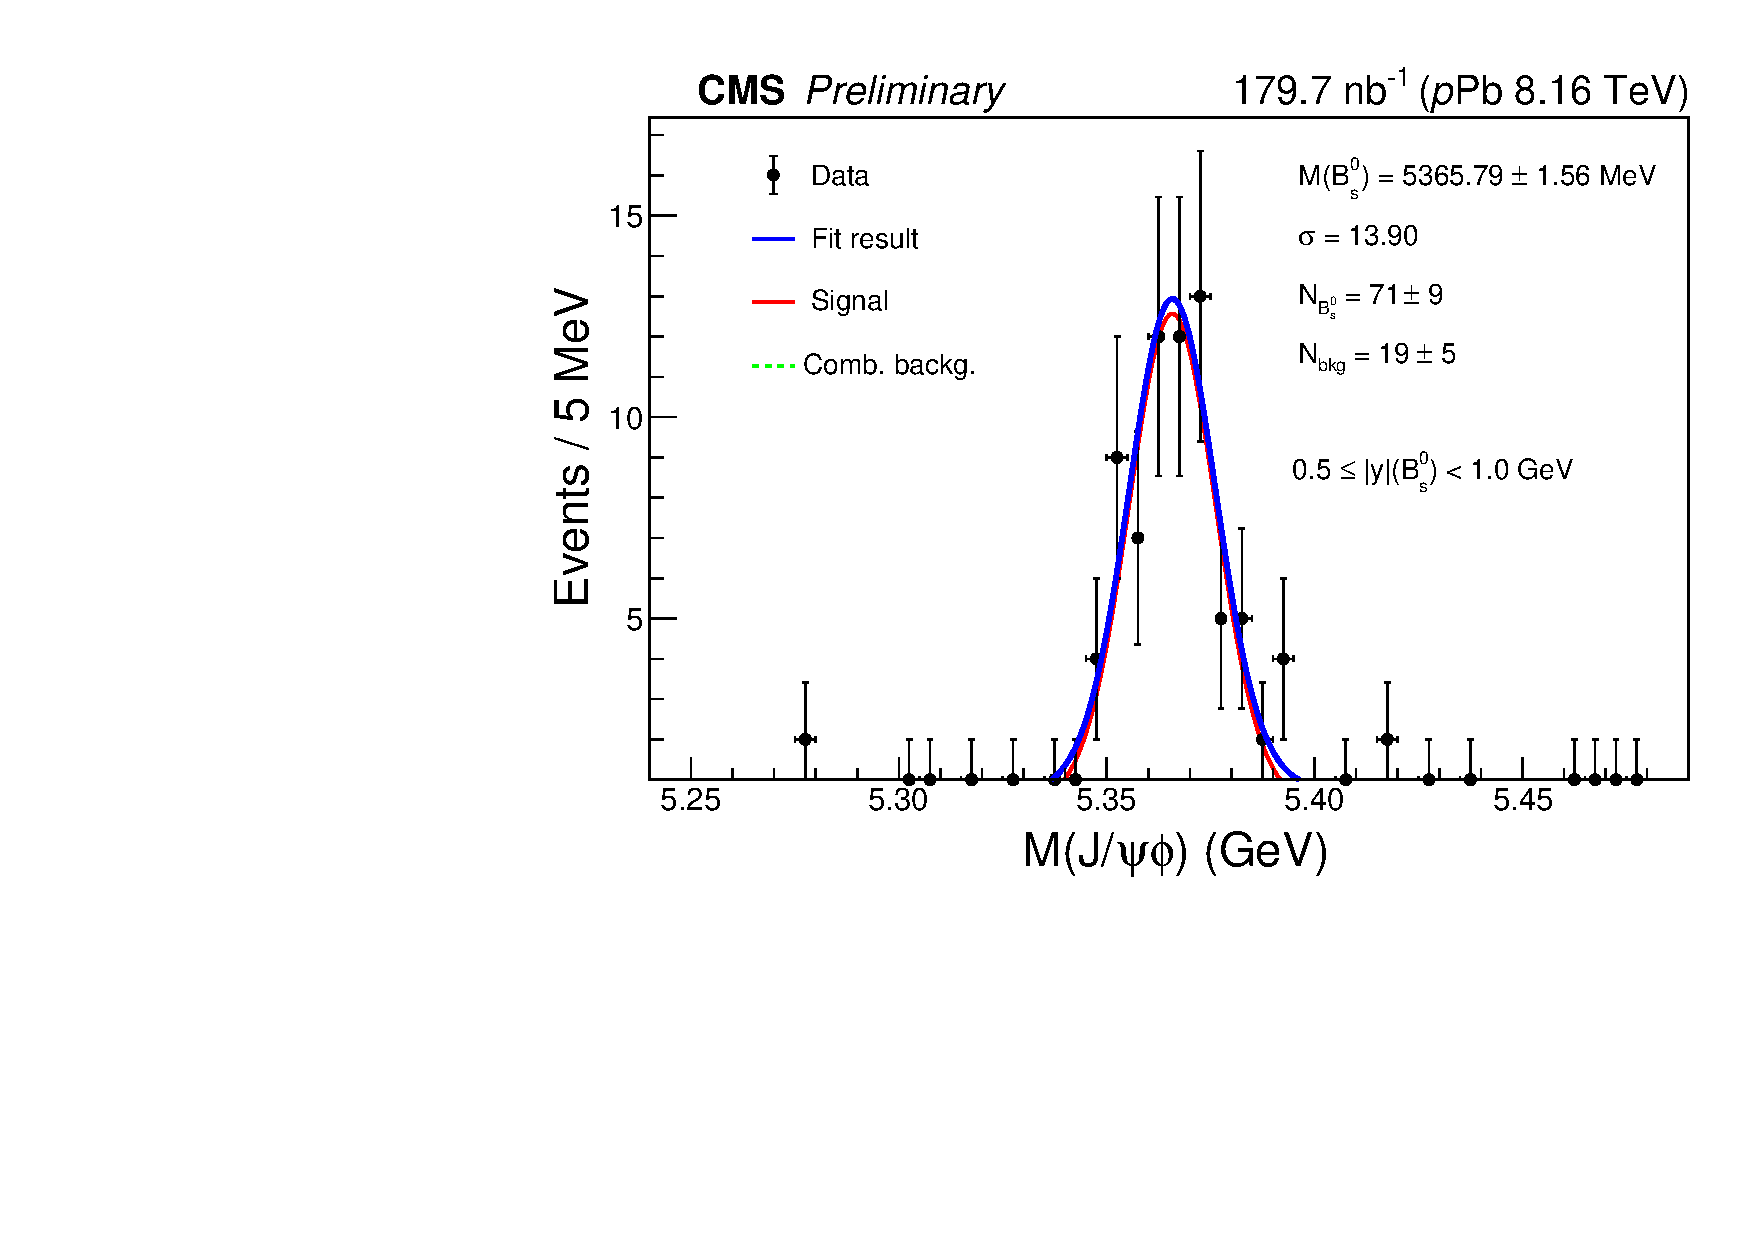
\includegraphics[width=\textwidth]{MainContent/Figs/mass/mass_BsFit_ybins_sysbkg_0.5_1.0.PDF}
		\caption{}%
		
	\end{subfigure}
	\vskip\baselineskip
	\begin{subfigure}[b]{0.475\textwidth}
		\centering
		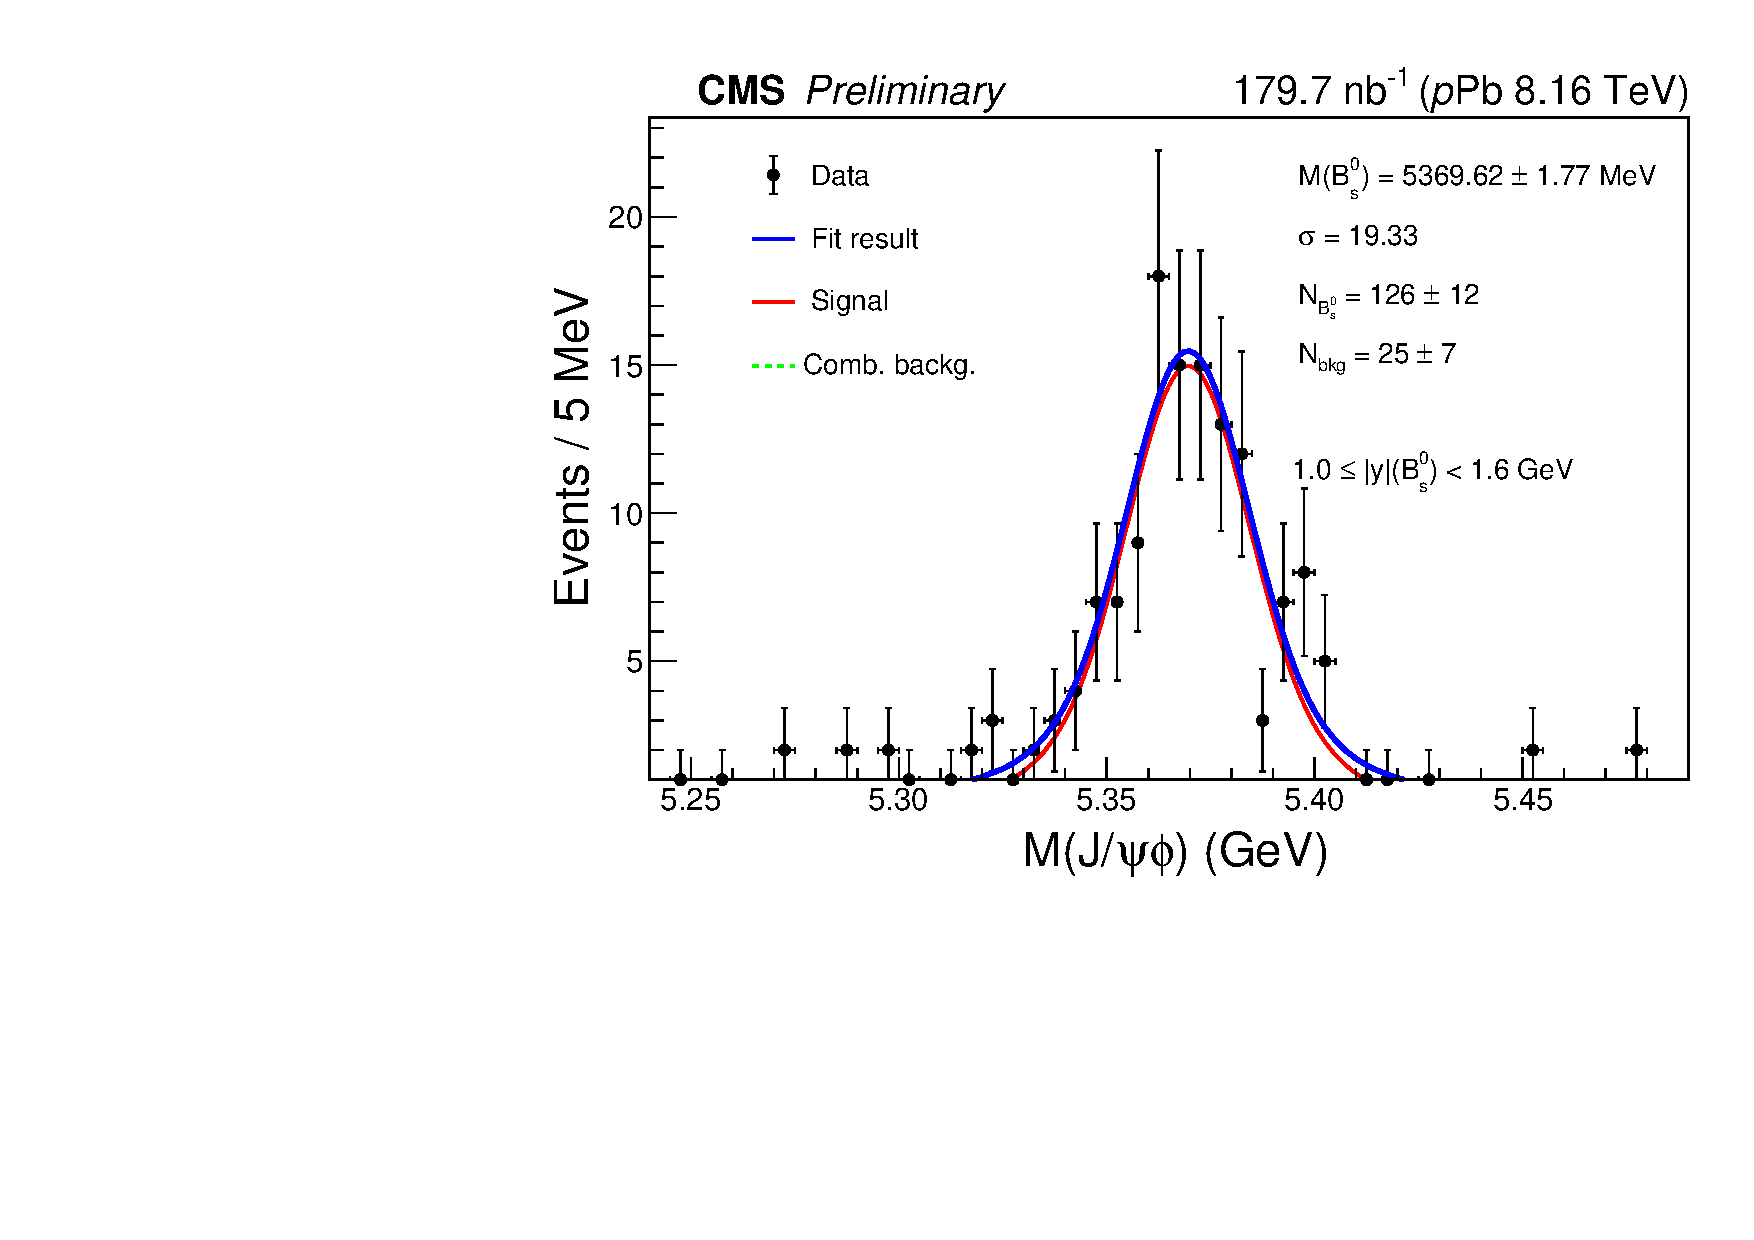
\includegraphics[width=\textwidth]{MainContent/Figs/mass/mass_BsFit_ybins_sysbkg_1.0_1.6.PDF}
		\caption{}
	\end{subfigure}
	\hfill
	\begin{subfigure}[b]{0.475\textwidth}
		\centering
		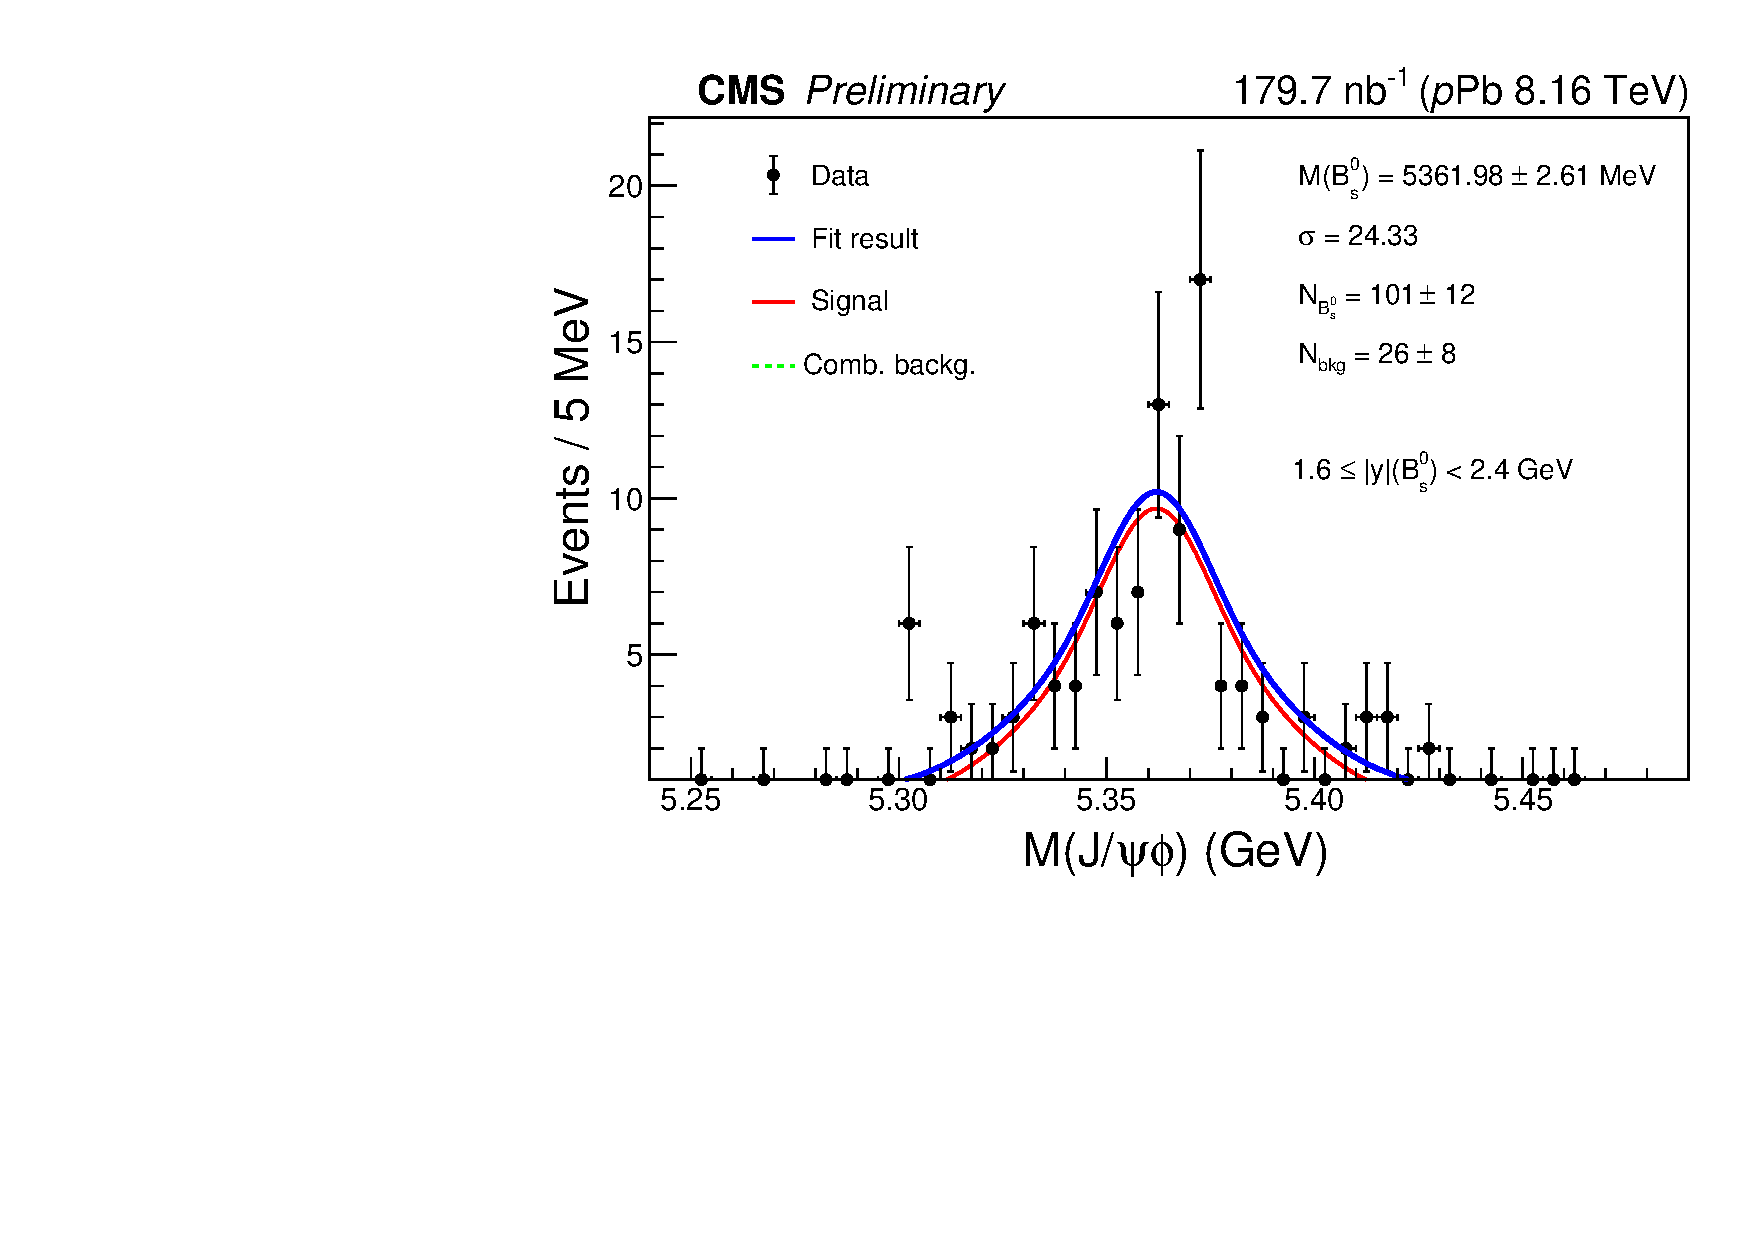
\includegraphics[width=\textwidth]{MainContent/Figs/mass/mass_BsFit_ybins_sysbkg_1.6_2.4.PDF}
		\caption{}%
	\end{subfigure}
	\caption{Invariant mass spectra for $B^0_s$ meson reconstructed from the combined system $J/\psi \phi$ and considering a systematic model for background. Four intervals for the rapidity $|y|(B^0_s)$ have been considered.}
	\label{fig:mass_ybins_sysbkg}
	%%%%%%%%%%%%%%%%%%%%%%%%%%%%%%%%%%%%second row
	
\end{figure}


\cleardoublepage
\subsection{Efficiency}

\subsubsection{MC size}
The uncertainties of the ratios defined for the acceptance and efficiency, $\delta \alpha$ and $\delta \epsilon$ are statistical. However, due to the finite size of the number of Monte Carlo samples used for reconstruction, they turn into systematic uncertainties when considering the differential cross-section. For practical purposes, the uncertainty of the total efficiency $\delta(\alpha \cdot \epsilon)$ is used instead of the individual uncertainties.


\subsubsection{Track}

The uncertainty in the efficiency of reconstruction of the tracks ($K^{+}K^{-}$) is considered a systematic uncertainty. In this paper, the value reported by \cite{cms2018tracking} will be used as the track efficiency uncertainty: $2.4\%$.

In the table \ref{table:Systematics}, the statistical and the systematic uncertainties considered for the cross-section are presented for each of the $p_T$ bins and in table \ref{table:Systematics_y} for the $|y|$ bins.
\begin{table}[htbp] \begin{center}\begin{tabular}{|c|c|c|c|c|c|c|}\hline$\mathbf{p_T}$    &  $\mathbf{N_{B_s^{0}}} $    &  $\mathbf{N_{B_s^{0}}} $  & \textbf{MC}   & \textbf{Tracking}  & \textbf{Total Systematic}  & \textbf{Statistical} \\\textbf{(GeV)}   & \textbf{signal}   & \textbf{bkg}    & \textbf{size} &           & \textbf{uncertainty} ($\mathbf{\%}$) & \textbf{uncertainty} ($\mathbf{\%}$) \\\hline{[}7, 10{)}  &  10.0  &  0.1 &  4.6  &  2.4 &  11.3 &  14.9 \\{[}10, 15{)}  &  8.1  &  0.1 &  2.5  &  2.4 &  8.8 &  10.2 \\{[}15, 20{)}  &  12.3  &  0.1 &  2.8  &  2.4 &  12.9 &  11.5 \\{[}20, 50{)}  &  26.0  &  0.0 &  2.7  &  2.4 &  26.2 &  10.8 \\\hline\end{tabular}\caption{Systematic uncertainties on  ${\frac{d \sigma}{dp_T}}$ from alternative fitting strategies described in the text. The total systematic uncertainty is the sum in quadrature of the individual uncertainties. Statistical uncertainty is show too.}\label{table:Systematics}\end{center}\end{table}

\begin{table}[htbp] \begin{center}\begin{tabular}{|c|c|c|c|c|c|c|}\hline$\mathbf{|y|}$    &  $\mathbf{N_{B_s^{0}}} $    &  $\mathbf{B_s^{0}} $  & \textbf{MC}   & \textbf{Tracking}  & \textbf{Total Systematic}  & \textbf{Statistical} \\\textbf{(GeV)}   & \textbf{signal}   & \textbf{bkg}    & \textbf{size} &           & \textbf{uncertainty} ($\mathbf{\%}$) & \textbf{uncertainty} ($\mathbf{\%}$) \\\hline{[}0.0, 0.5{)}  &  0.1  &  0.1 &  3.2  &  2.4 &  4.0 &  12.3 \\{[}0.5, 1.0{)}  &  2.3  &  0.4 &  3.1  &  2.4 &  4.6 &  12.6 \\{[}1.0, 1.6{)}  &  0.8  &  0.2 &  2.6  &  2.4 &  3.6 &  9.6 \\{[}1.6, 2.4{)}  &  25.1  &  0.2 &  3.1  &  2.4 &  25.4 &  11.7 \\\hline\end{tabular}\caption{Systematic uncertainties on  ${\frac{d \sigma}{d|y|}}$ from alternative fitting strategies described in the text. Statistical uncertainty is show too.}\label{table:Systematics_y}\end{center}\end{table}

% Chapter 6
\chapter[\leavevmode\newline Results]{Results}
\chaptermark{Results}
\label{chap:Chapter_6}

\section{Invariant mass distribution of $B^0_S$}
\subsection{$p_T$ bins}

\begin{figure}
	\centering
	\begin{subfigure}[t]{0.8\textwidth}
		\raisebox{-\height}{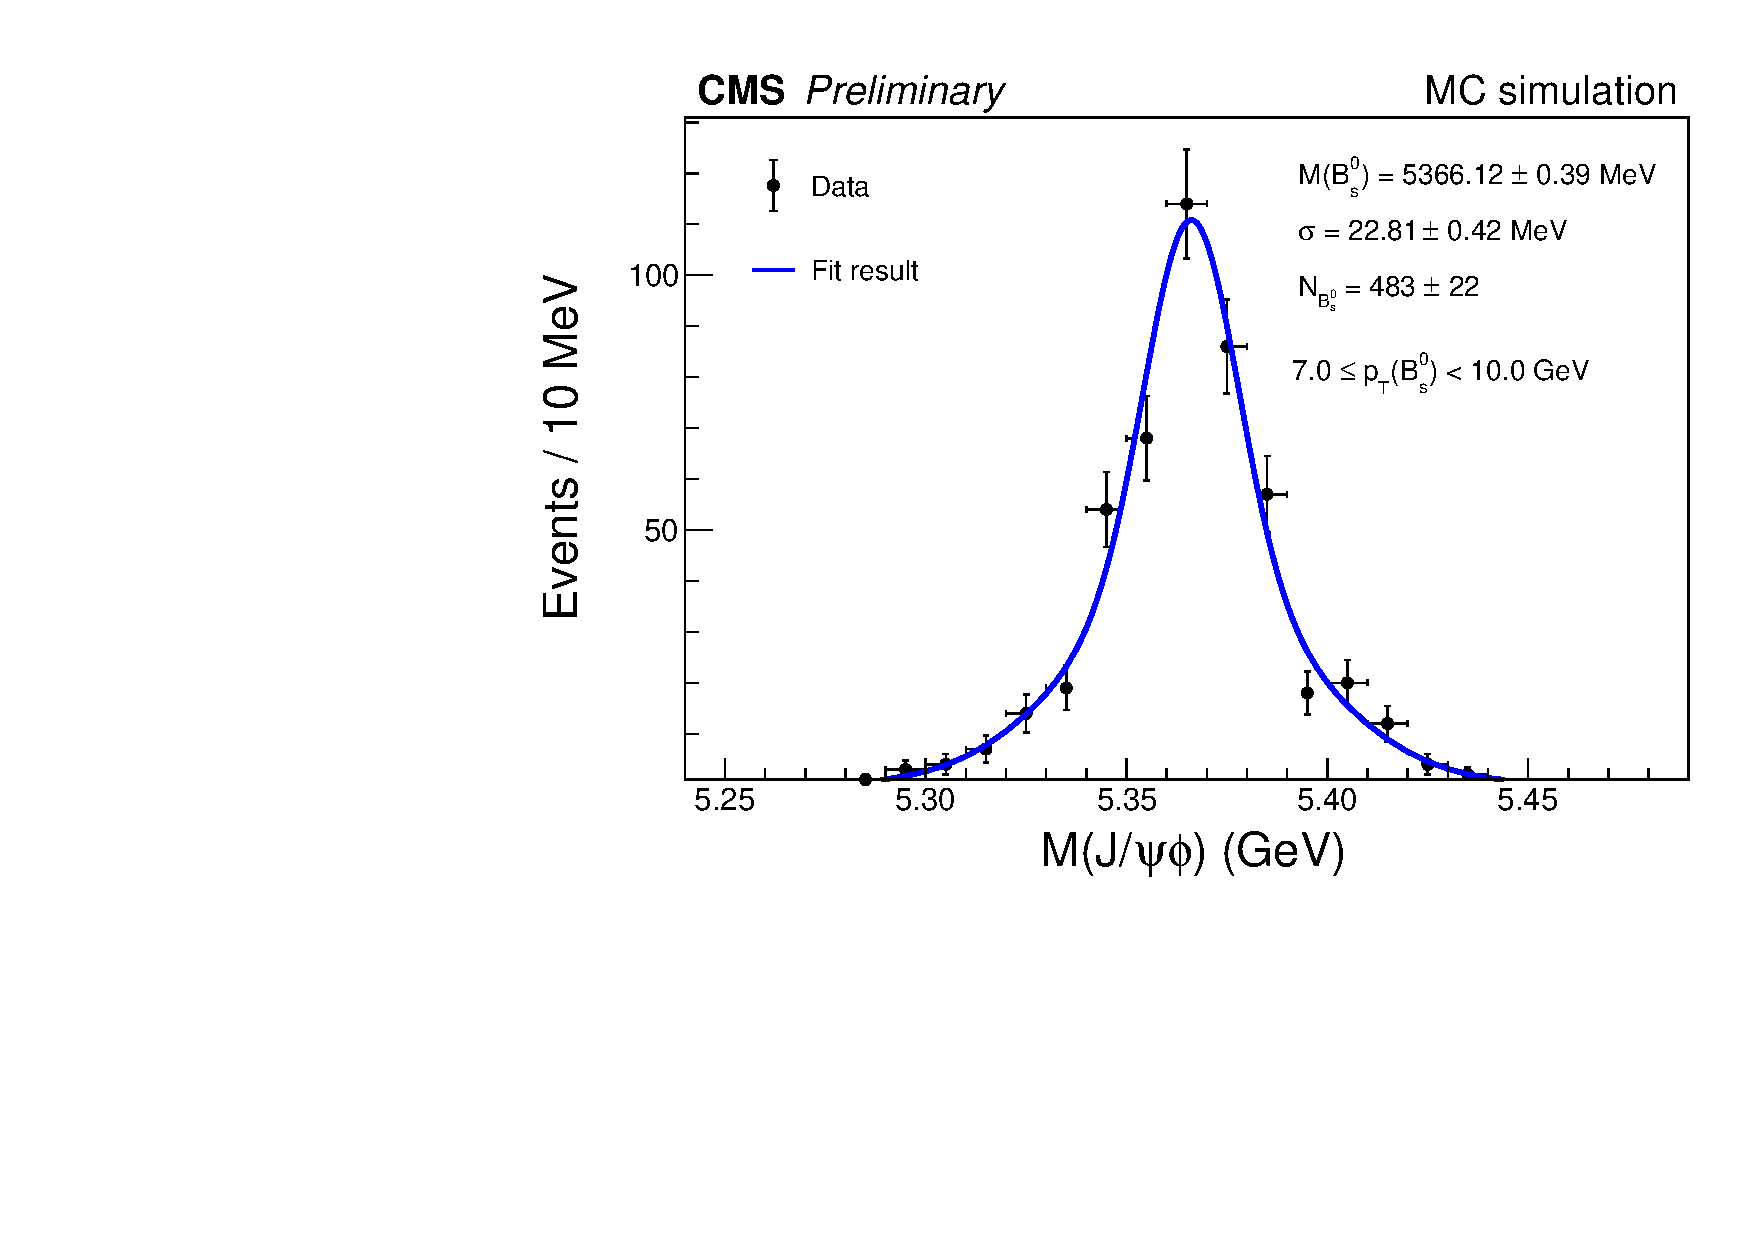
\includegraphics[width=0.49\textwidth]{MainContent/Figs/mass/mass_BsFitMC_best1_ptbins_7_10.PDF}}
		\raisebox{-\height}{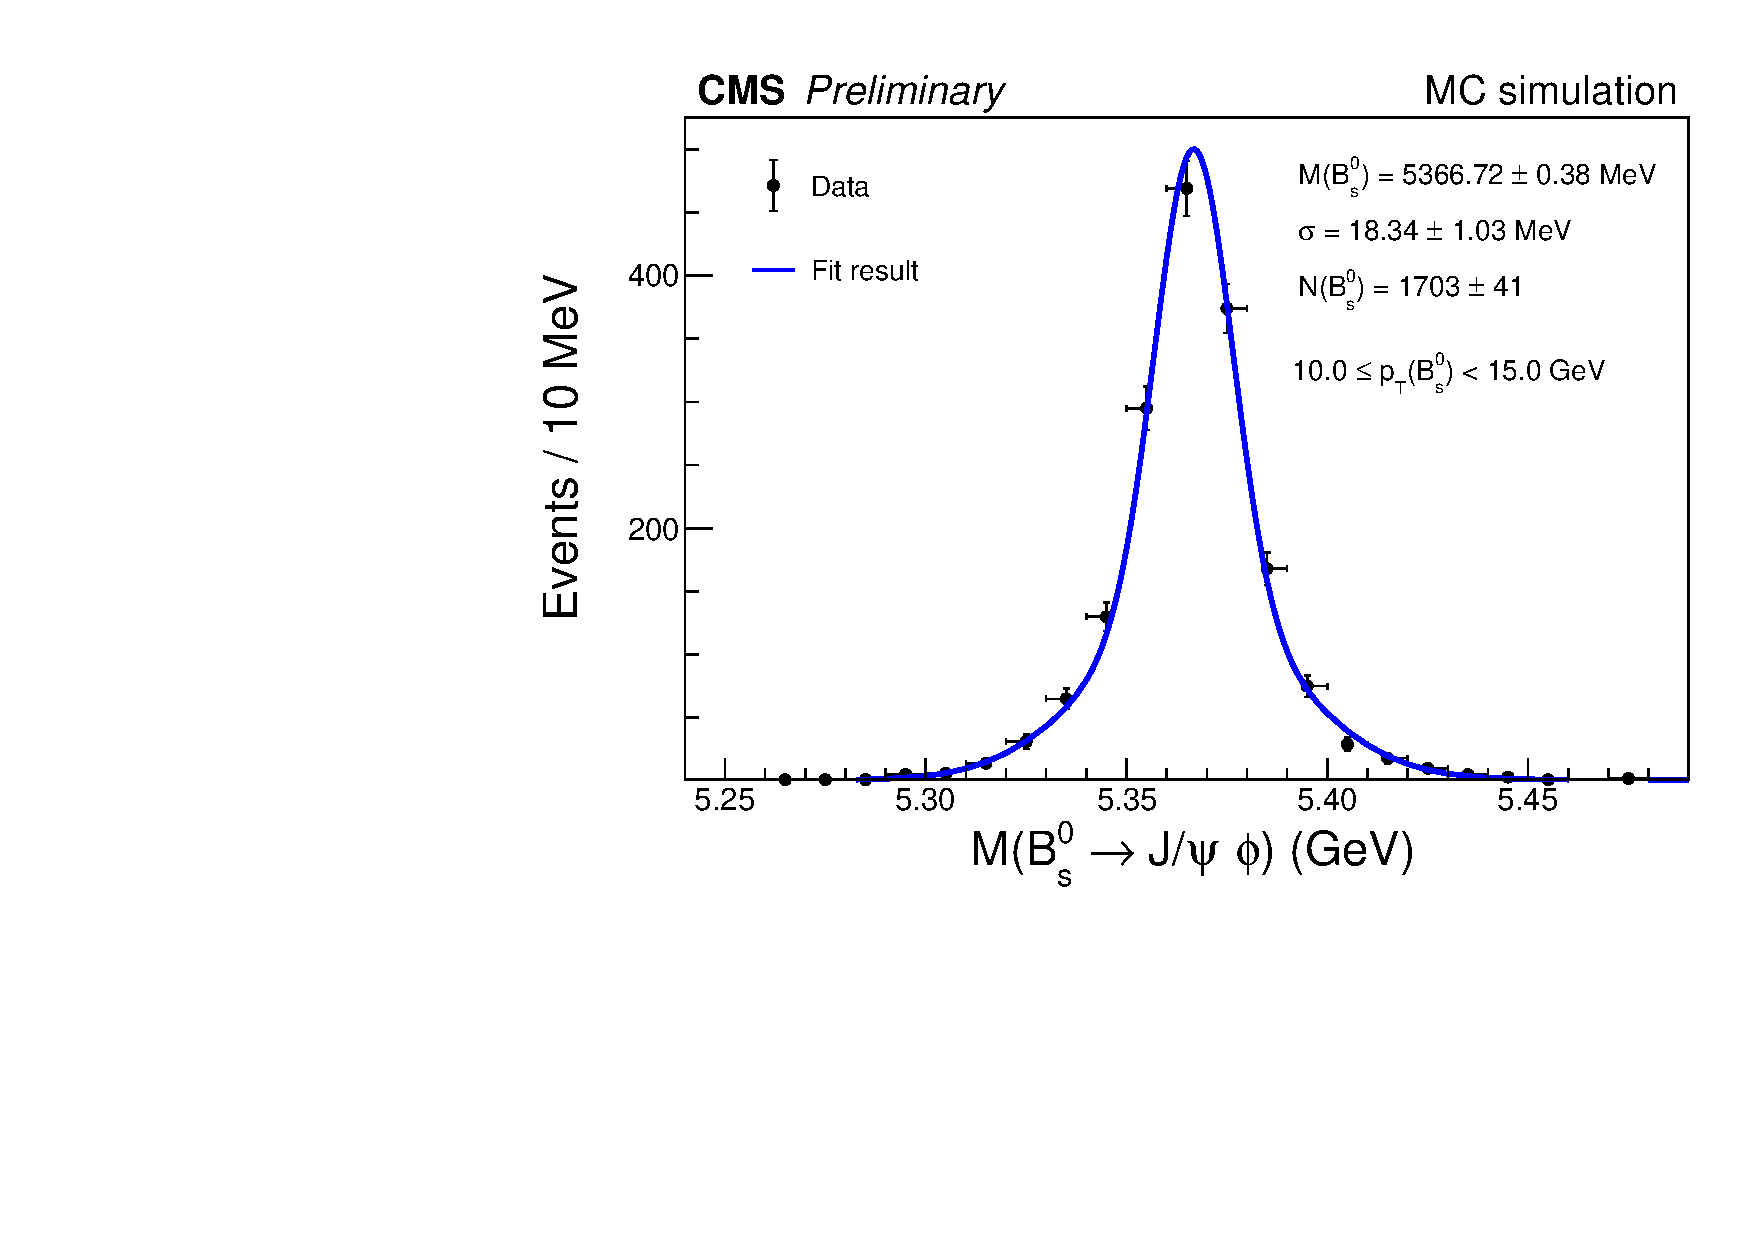
\includegraphics[width=0.49\textwidth]{MainContent/Figs/mass/mass_BsFitMC_best1_ptbins_10_15.PDF}}%
		\vspace{.6ex}
			\raisebox{-\height}{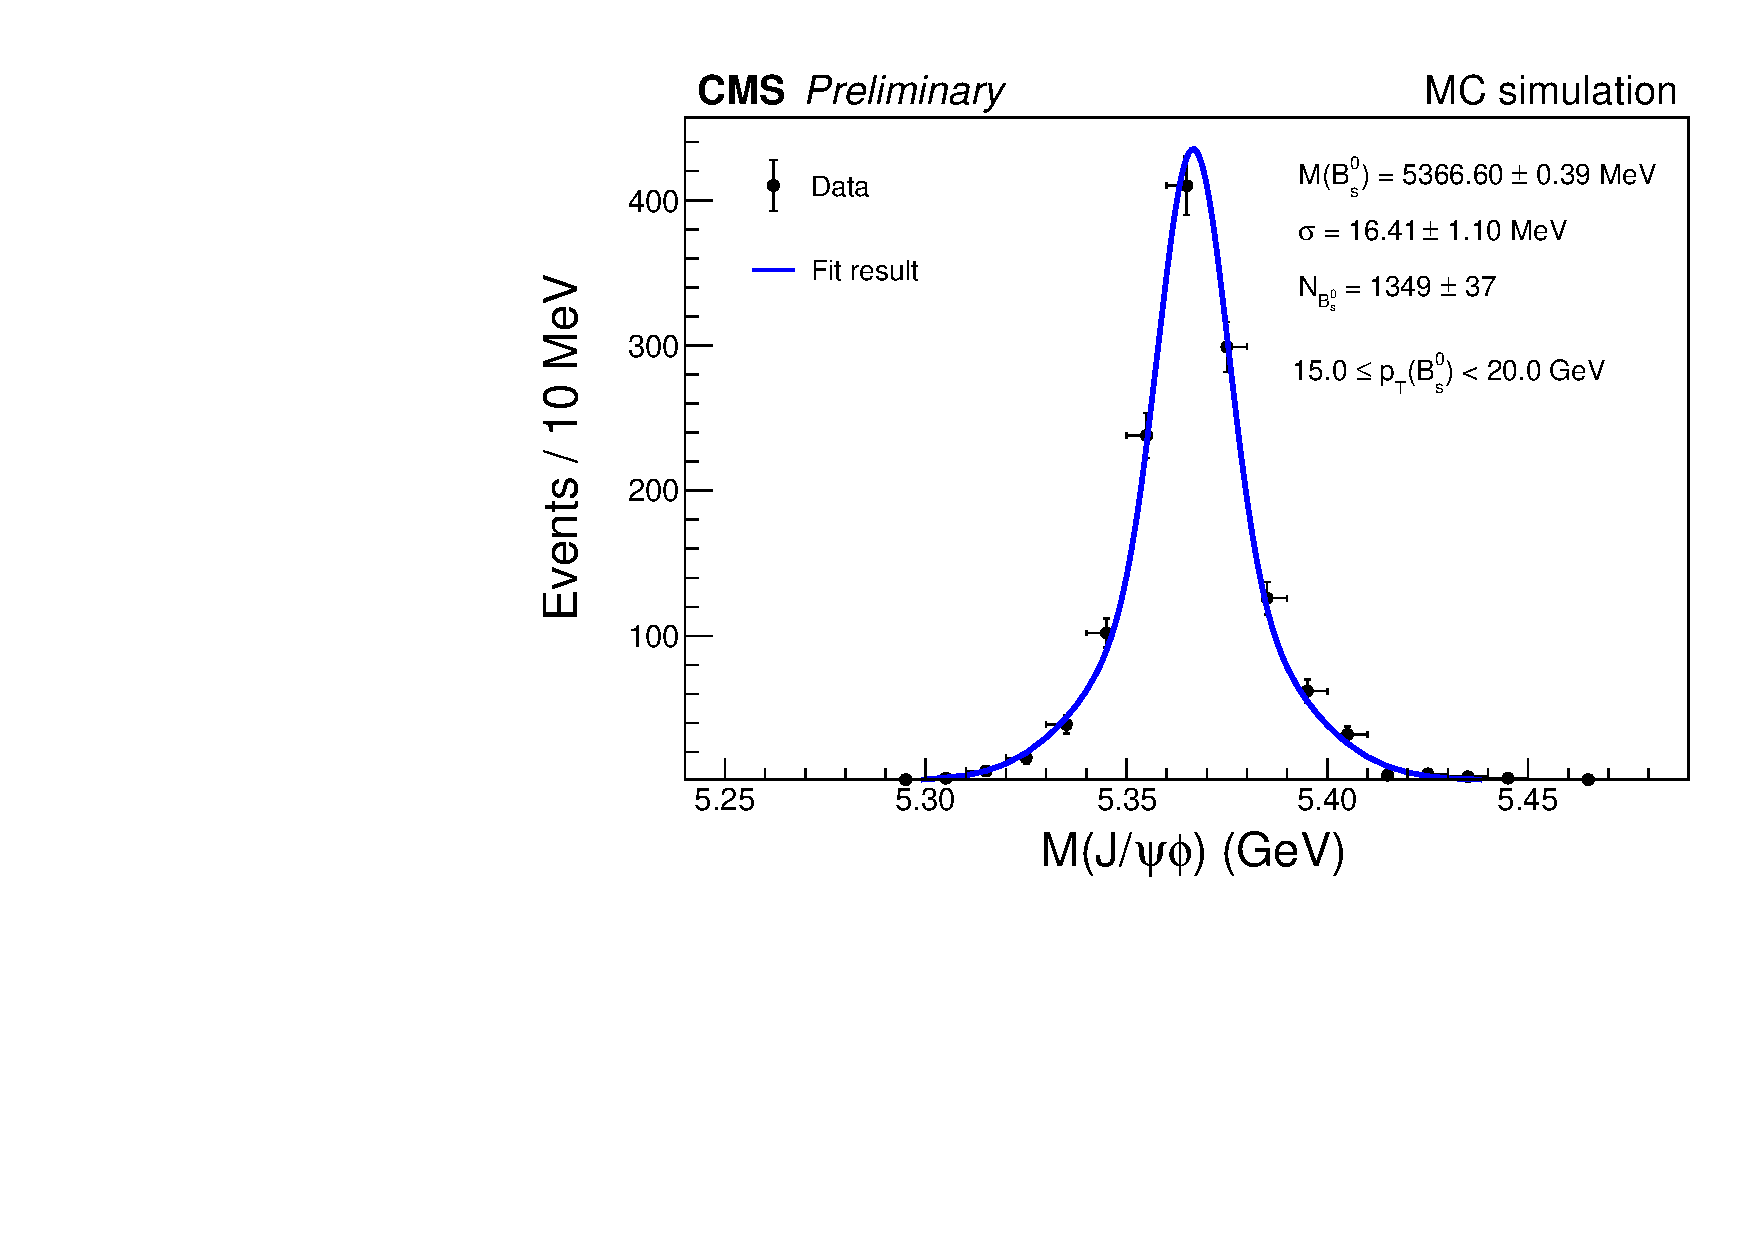
\includegraphics[width=0.49\textwidth]{MainContent/Figs/mass/mass_BsFitMC_best1_ptbins_15_20.PDF}}
		\raisebox{-\height}{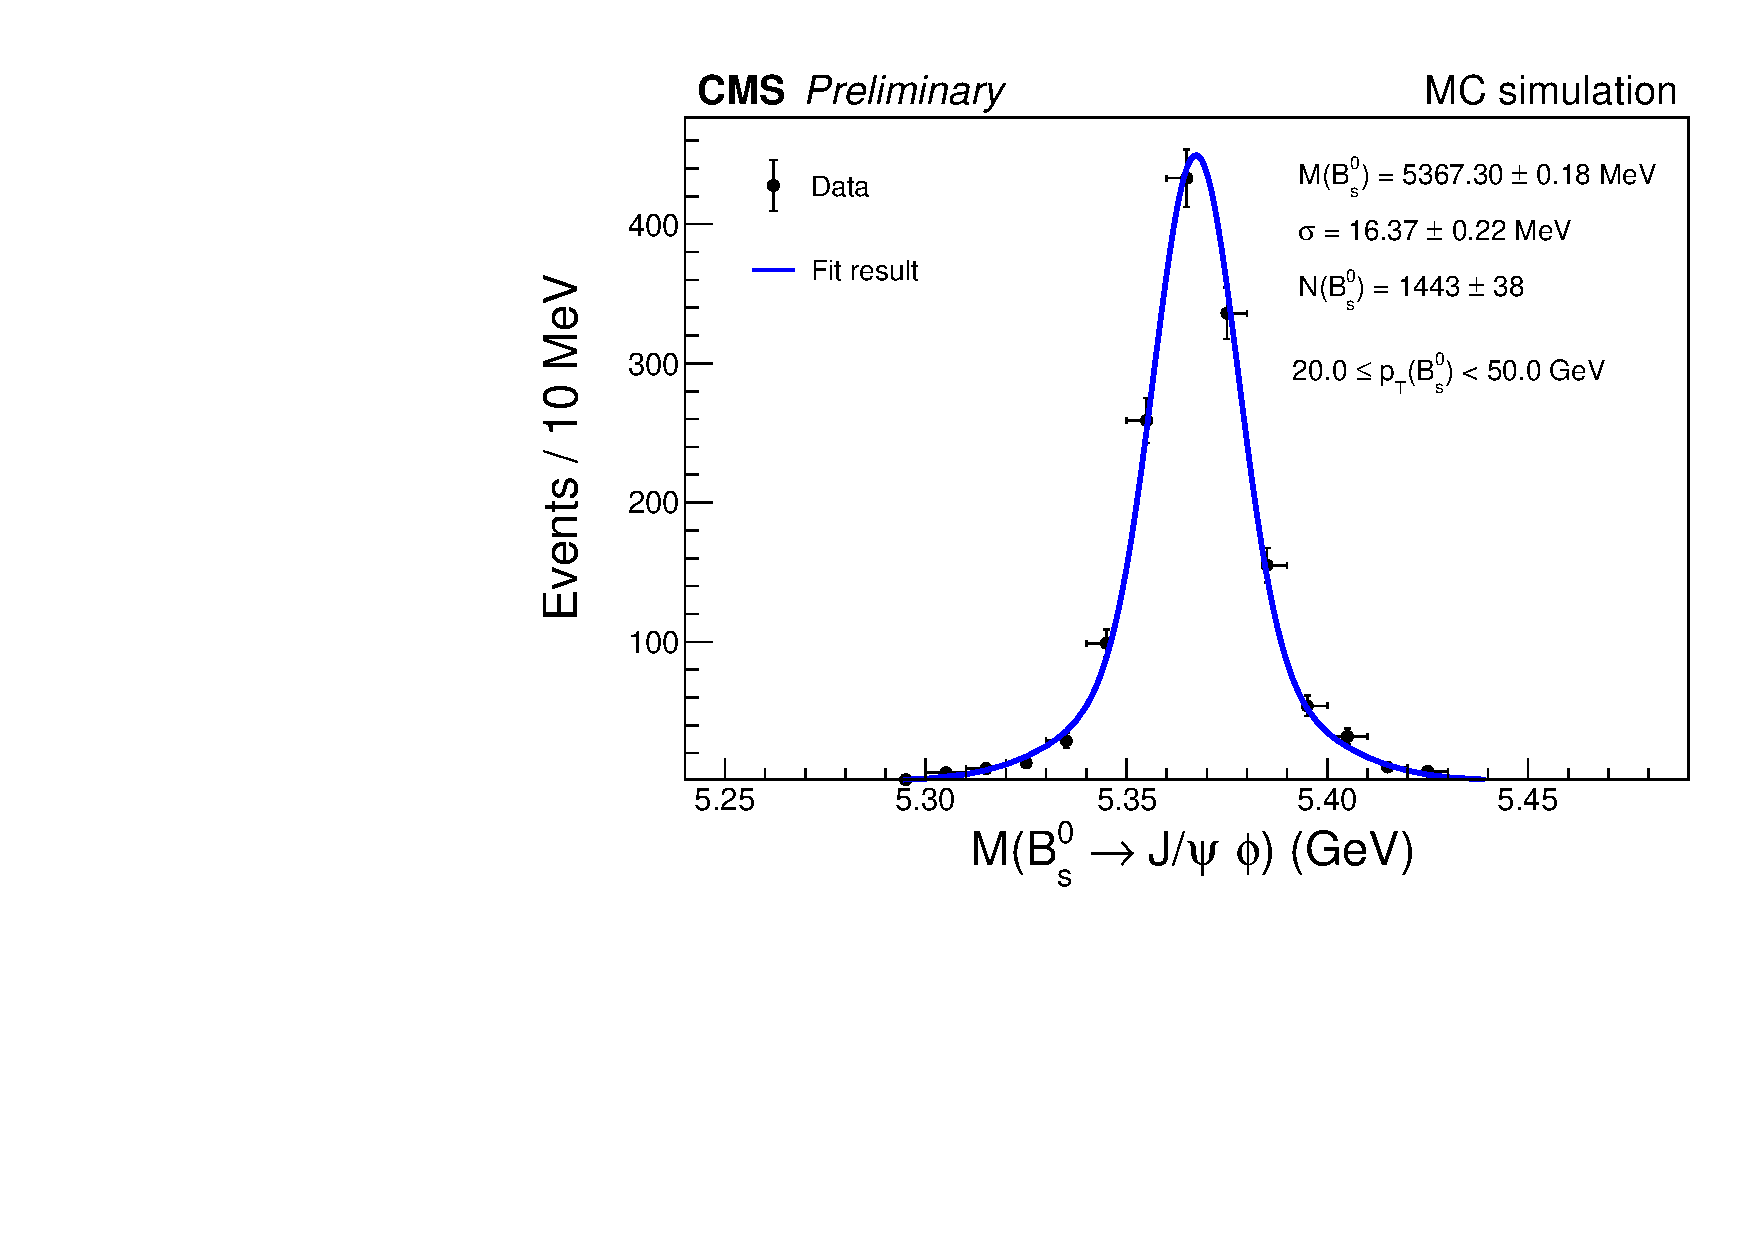
\includegraphics[width=0.49\textwidth]{MainContent/Figs/mass/mass_BsFitMC_best1_ptbins_20_50.PDF}}%
	\end{subfigure}
	\hfill
	\begin{subfigure}[t]{0.8\textwidth}
		\raisebox{-\height}{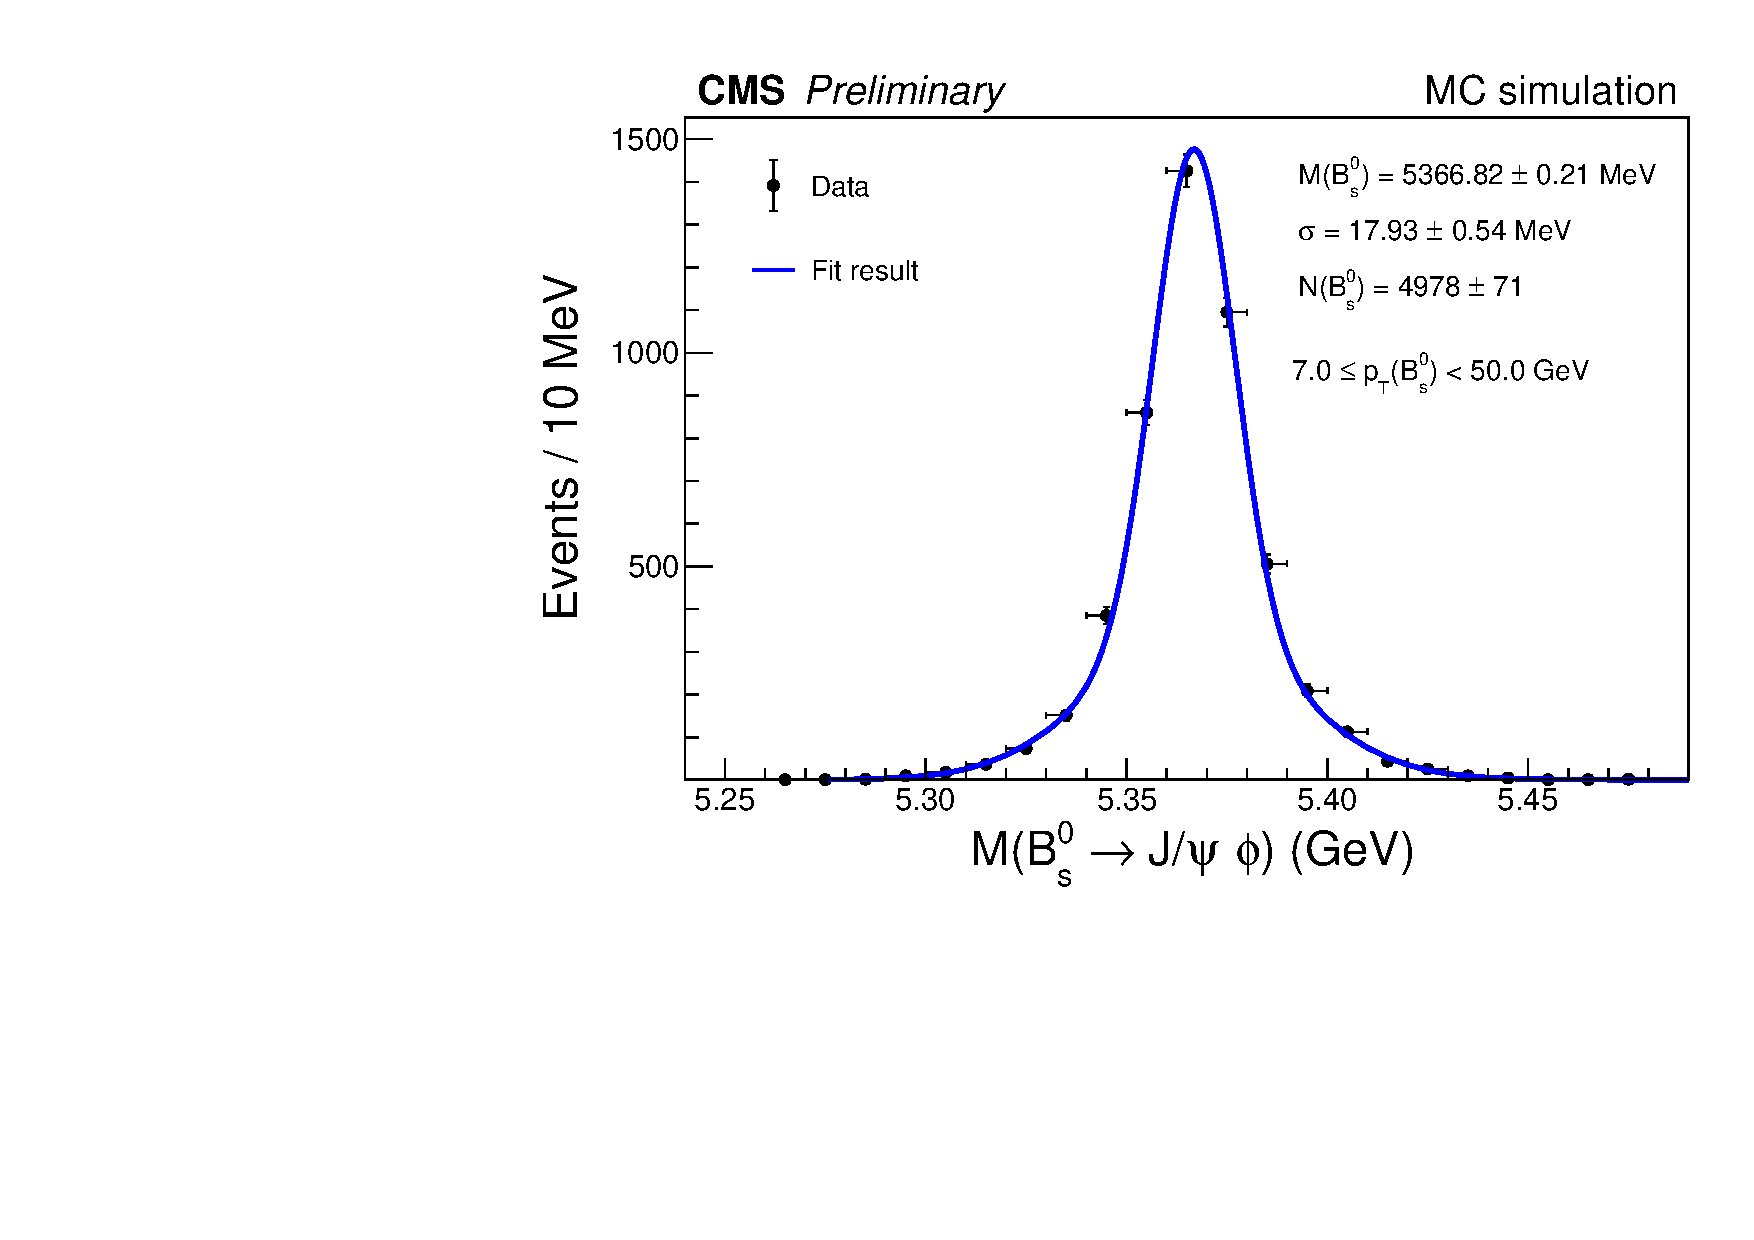
\includegraphics[width=\textwidth]{MainContent/Figs/mass/mass_BsFitMC_best1_ptbins_7_50.PDF}}
		
	\end{subfigure}
	\caption{Invariant mass spectra for the $B^0_s$ meson using the data from the MC simulation and considering the different bins for $p_T$. }
	%%%%%%%%%%%%%%%%%%%%%%%%%%%%%%%%%%%%second row
	
\end{figure}


\begin{figure}
	\centering
	\begin{subfigure}[t]{0.8\textwidth}
		\raisebox{-\height}{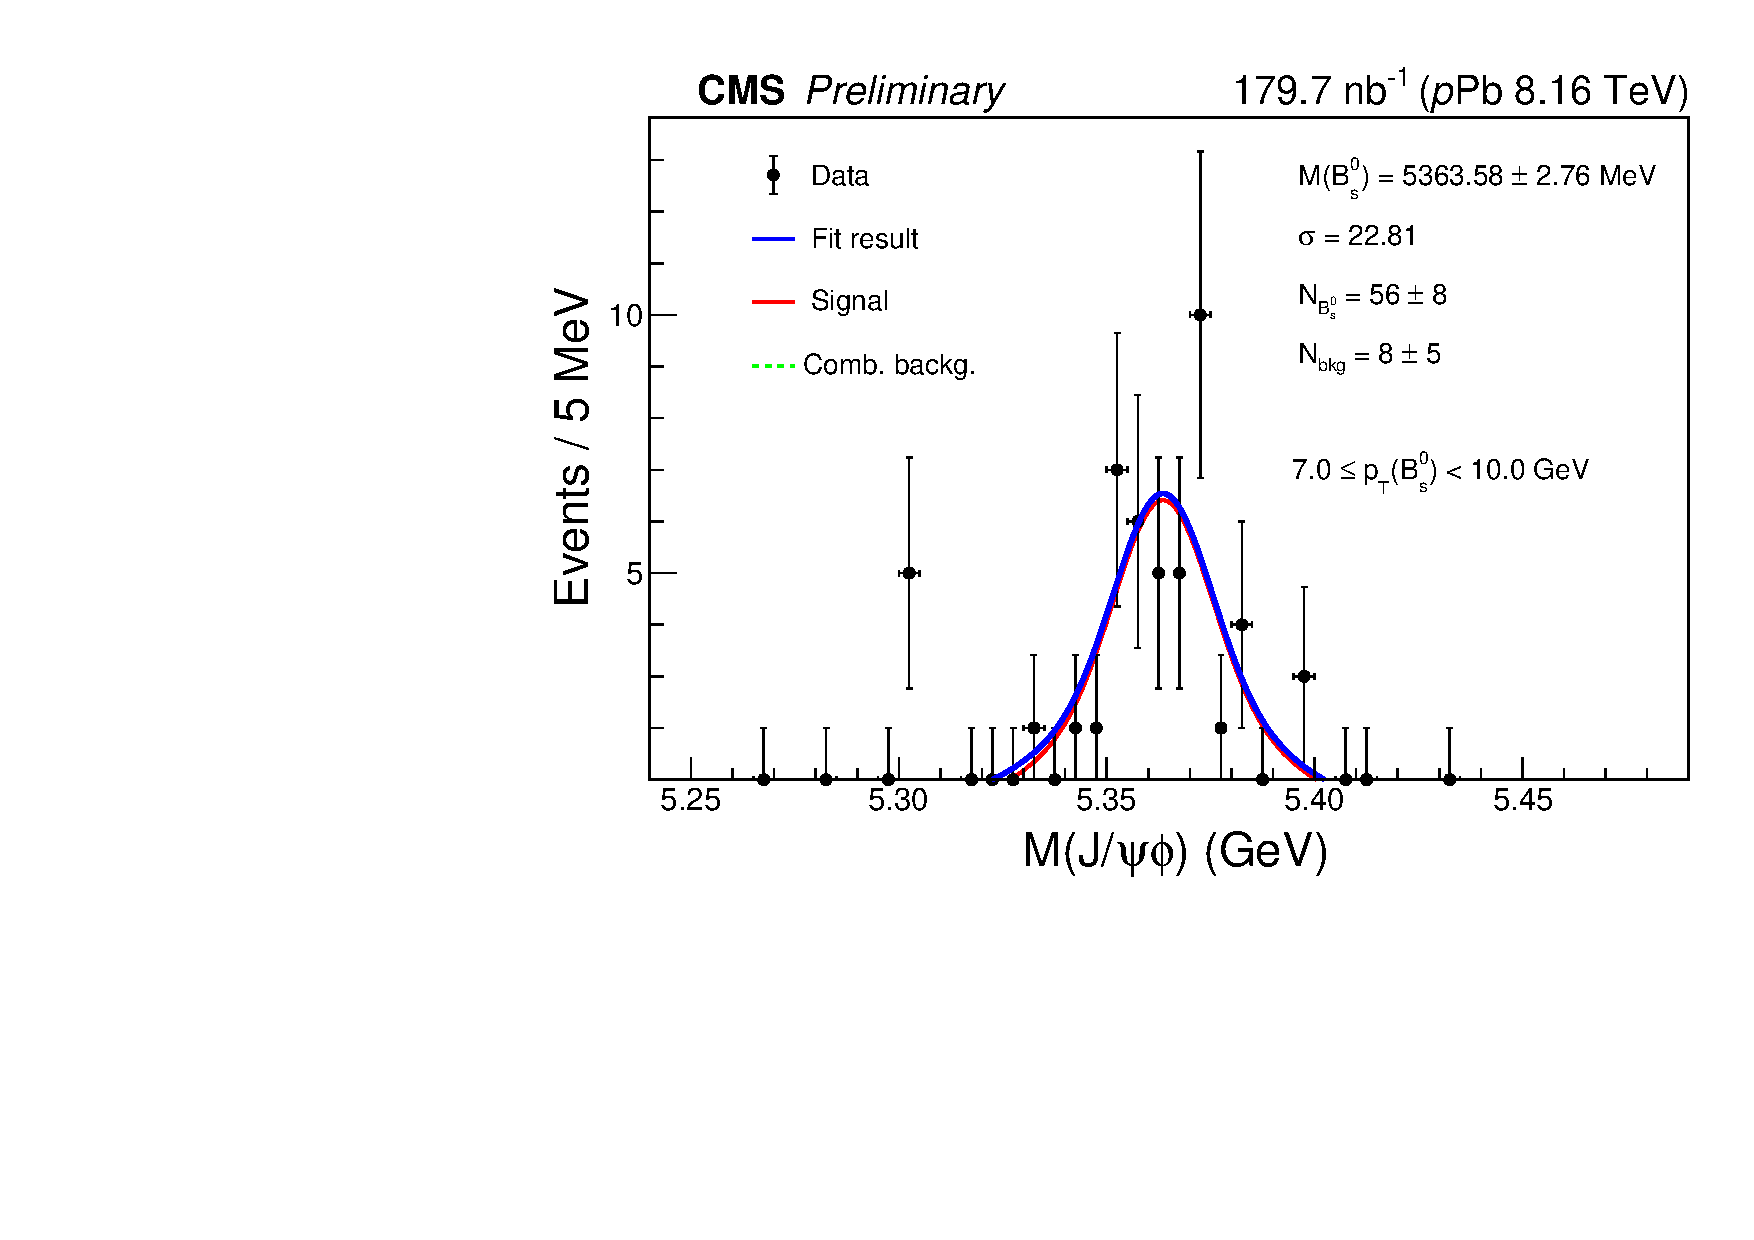
\includegraphics[width=0.49\textwidth]{MainContent/Figs/mass/mass_BsFit_ptbins_7_10.PDF}}
		\raisebox{-\height}{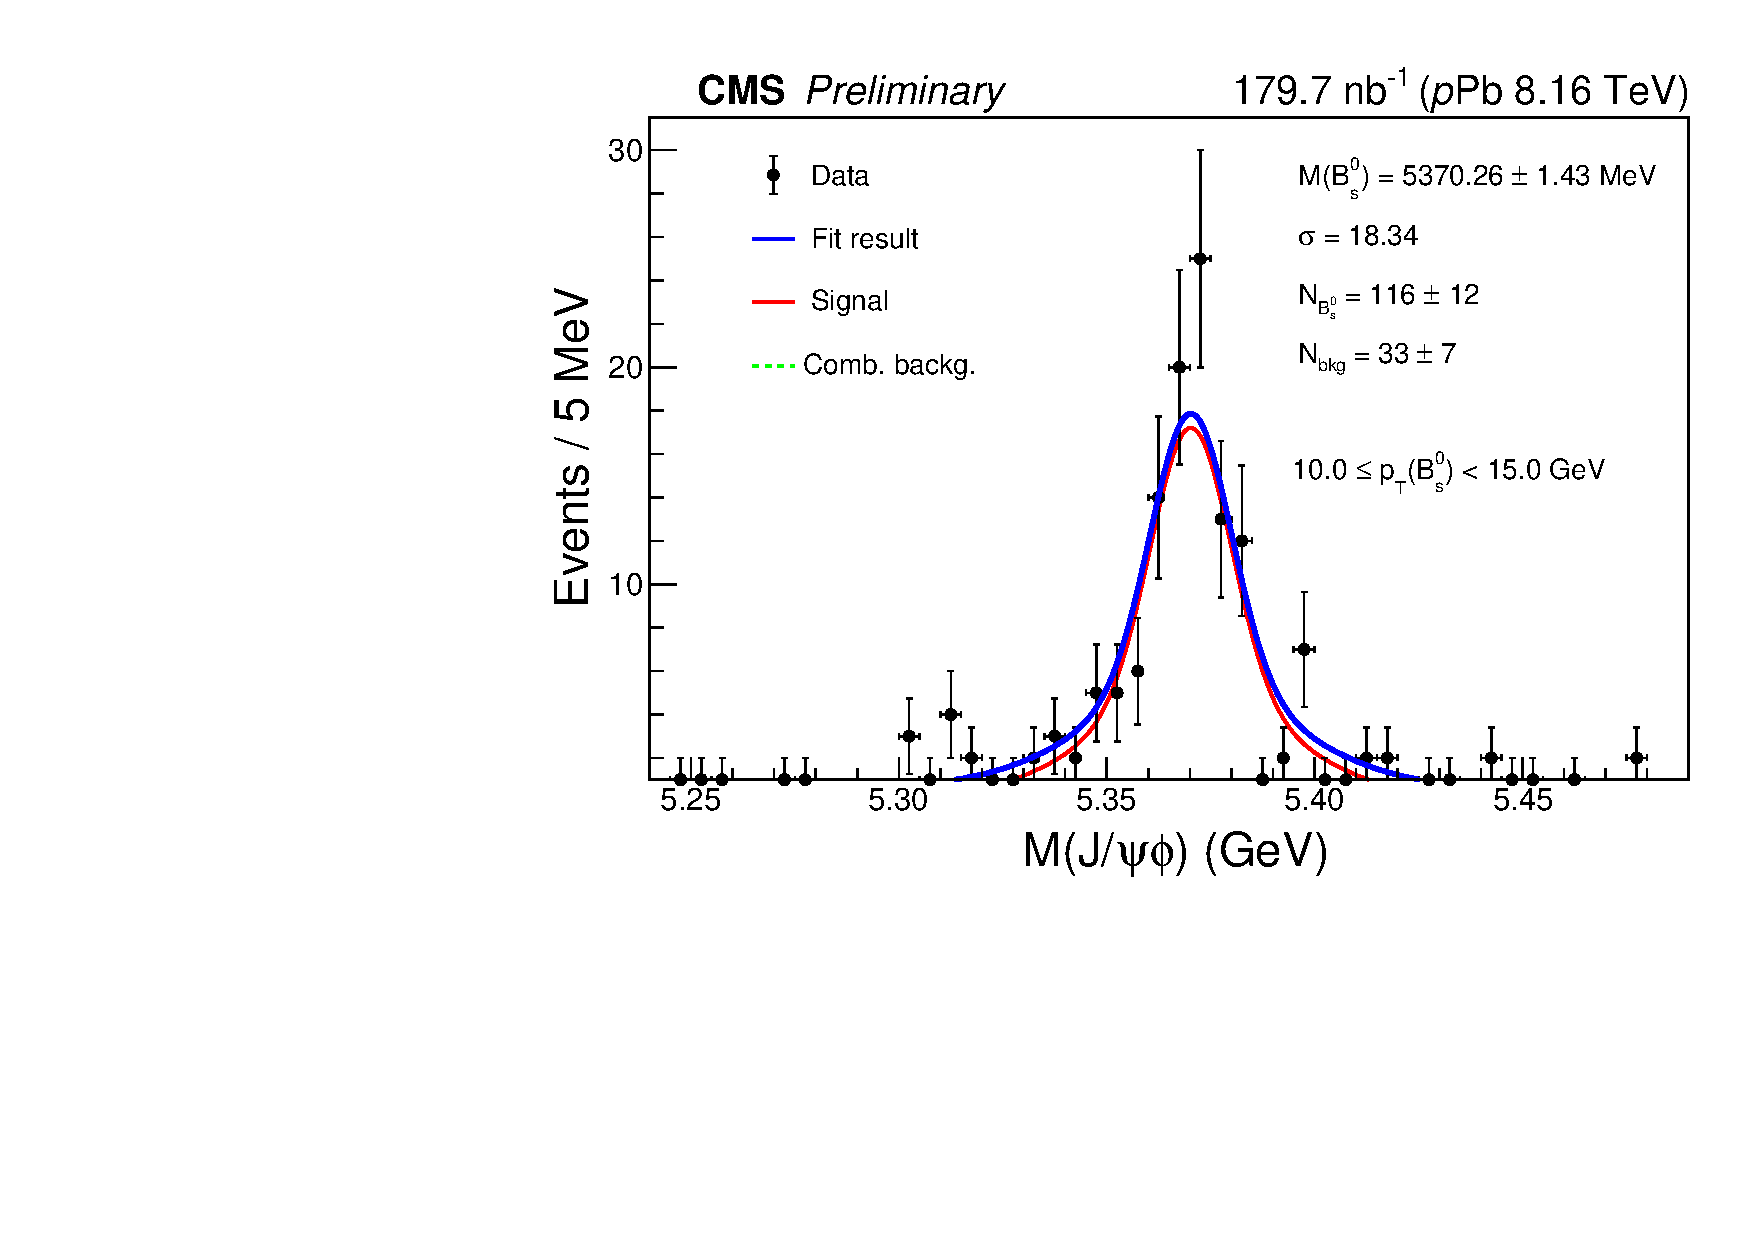
\includegraphics[width=0.49\textwidth]{MainContent/Figs/mass/mass_BsFit_ptbins_10_15.PDF}}%
		\vspace{.6ex}
		\raisebox{-\height}{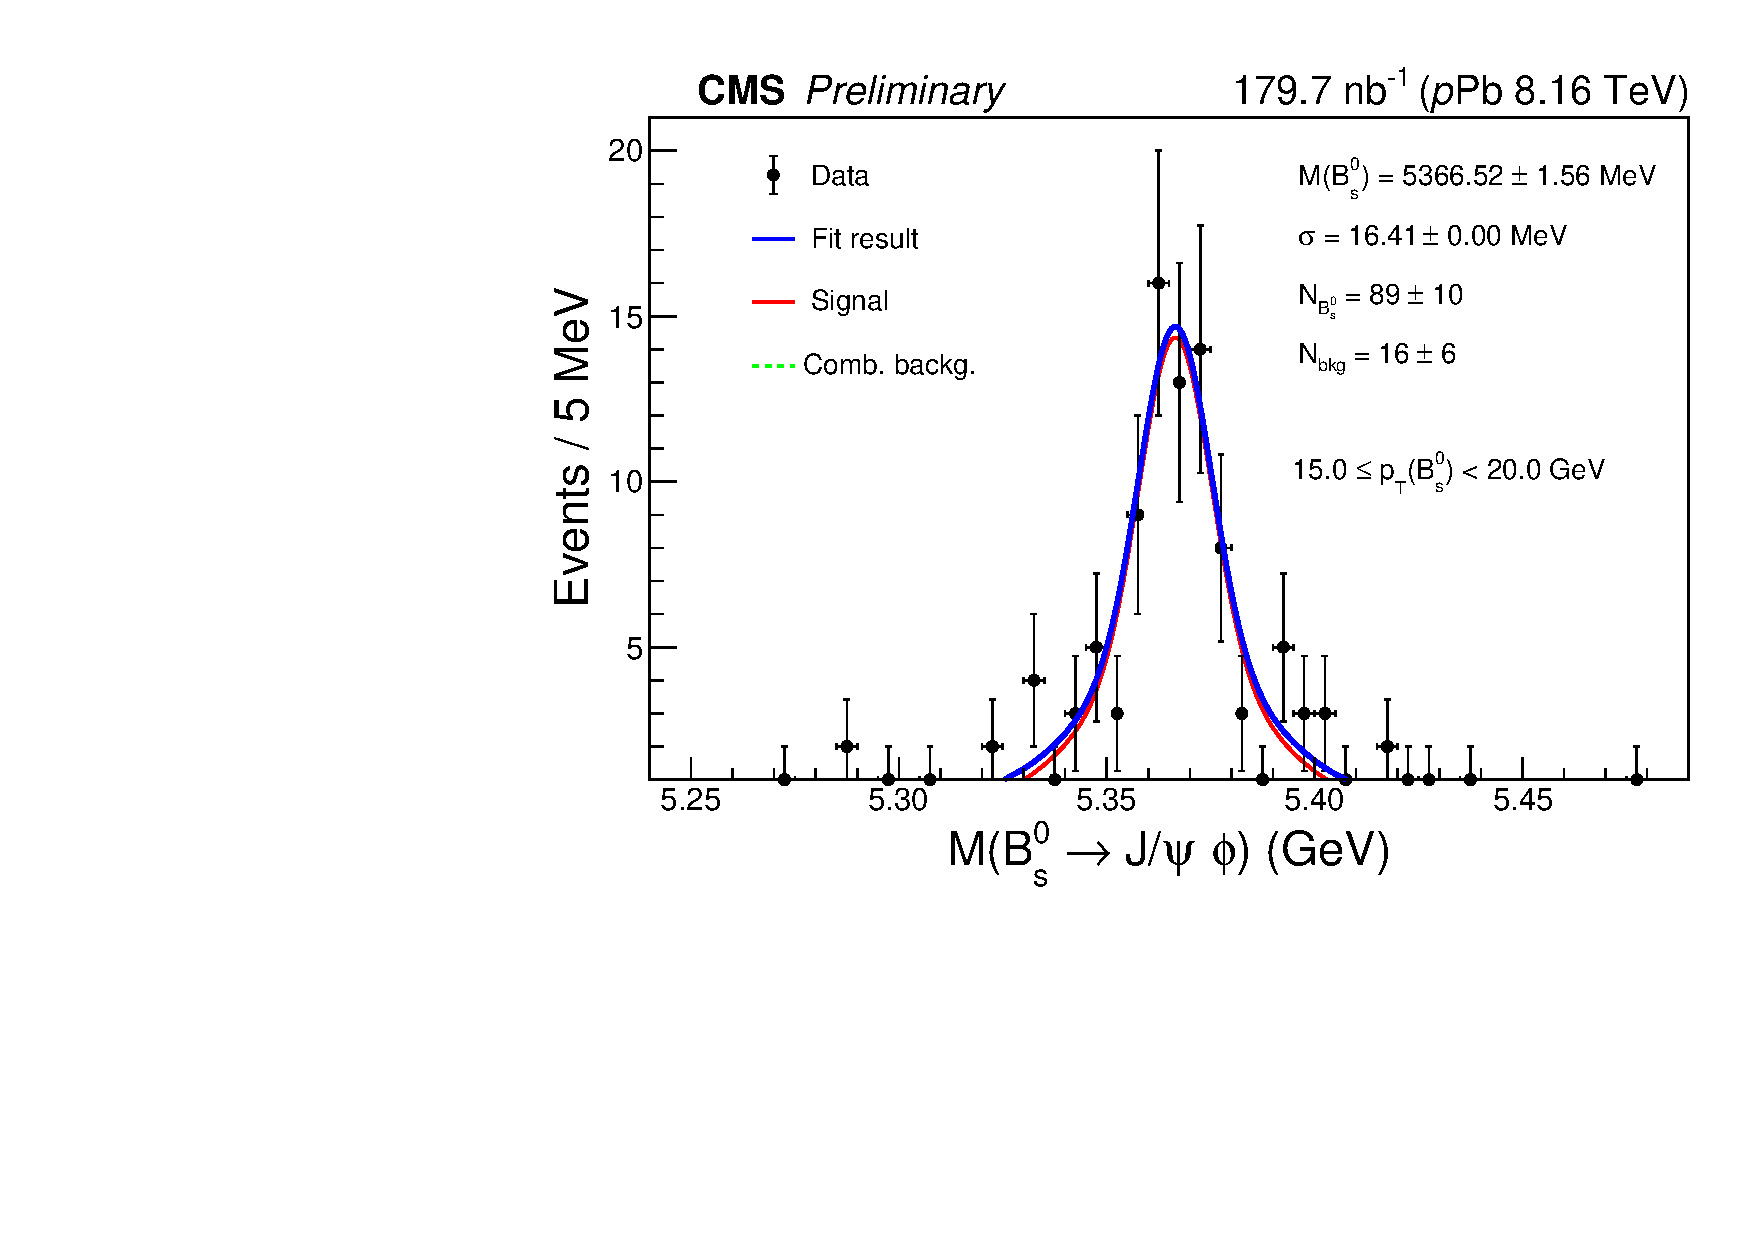
\includegraphics[width=0.49\textwidth]{MainContent/Figs/mass/mass_BsFit_ptbins_15_20.PDF}}
		\raisebox{-\height}{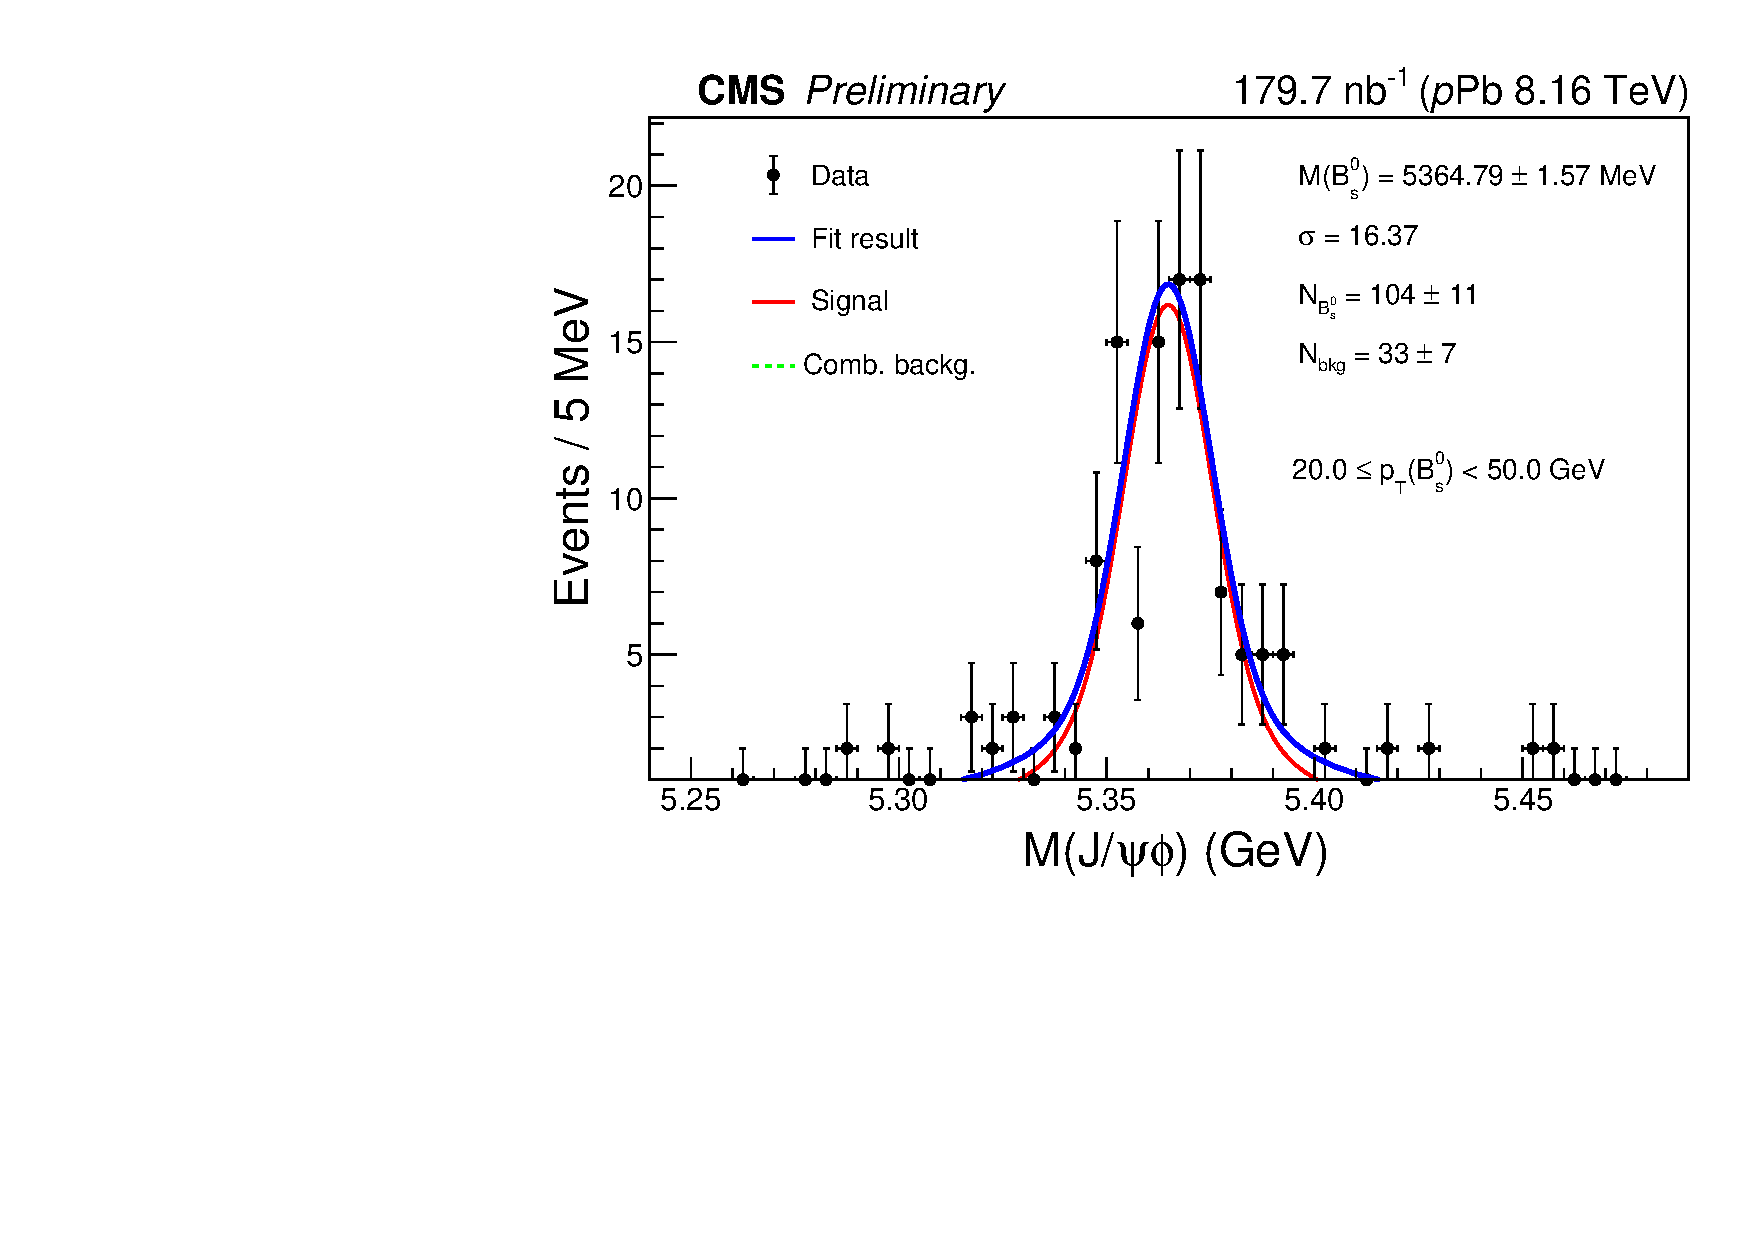
\includegraphics[width=0.49\textwidth]{MainContent/Figs/mass/mass_BsFit_ptbins_20_50.PDF}}%
	\end{subfigure}
	\hfill
	\begin{subfigure}[t]{0.8\textwidth}
		\raisebox{-\height}{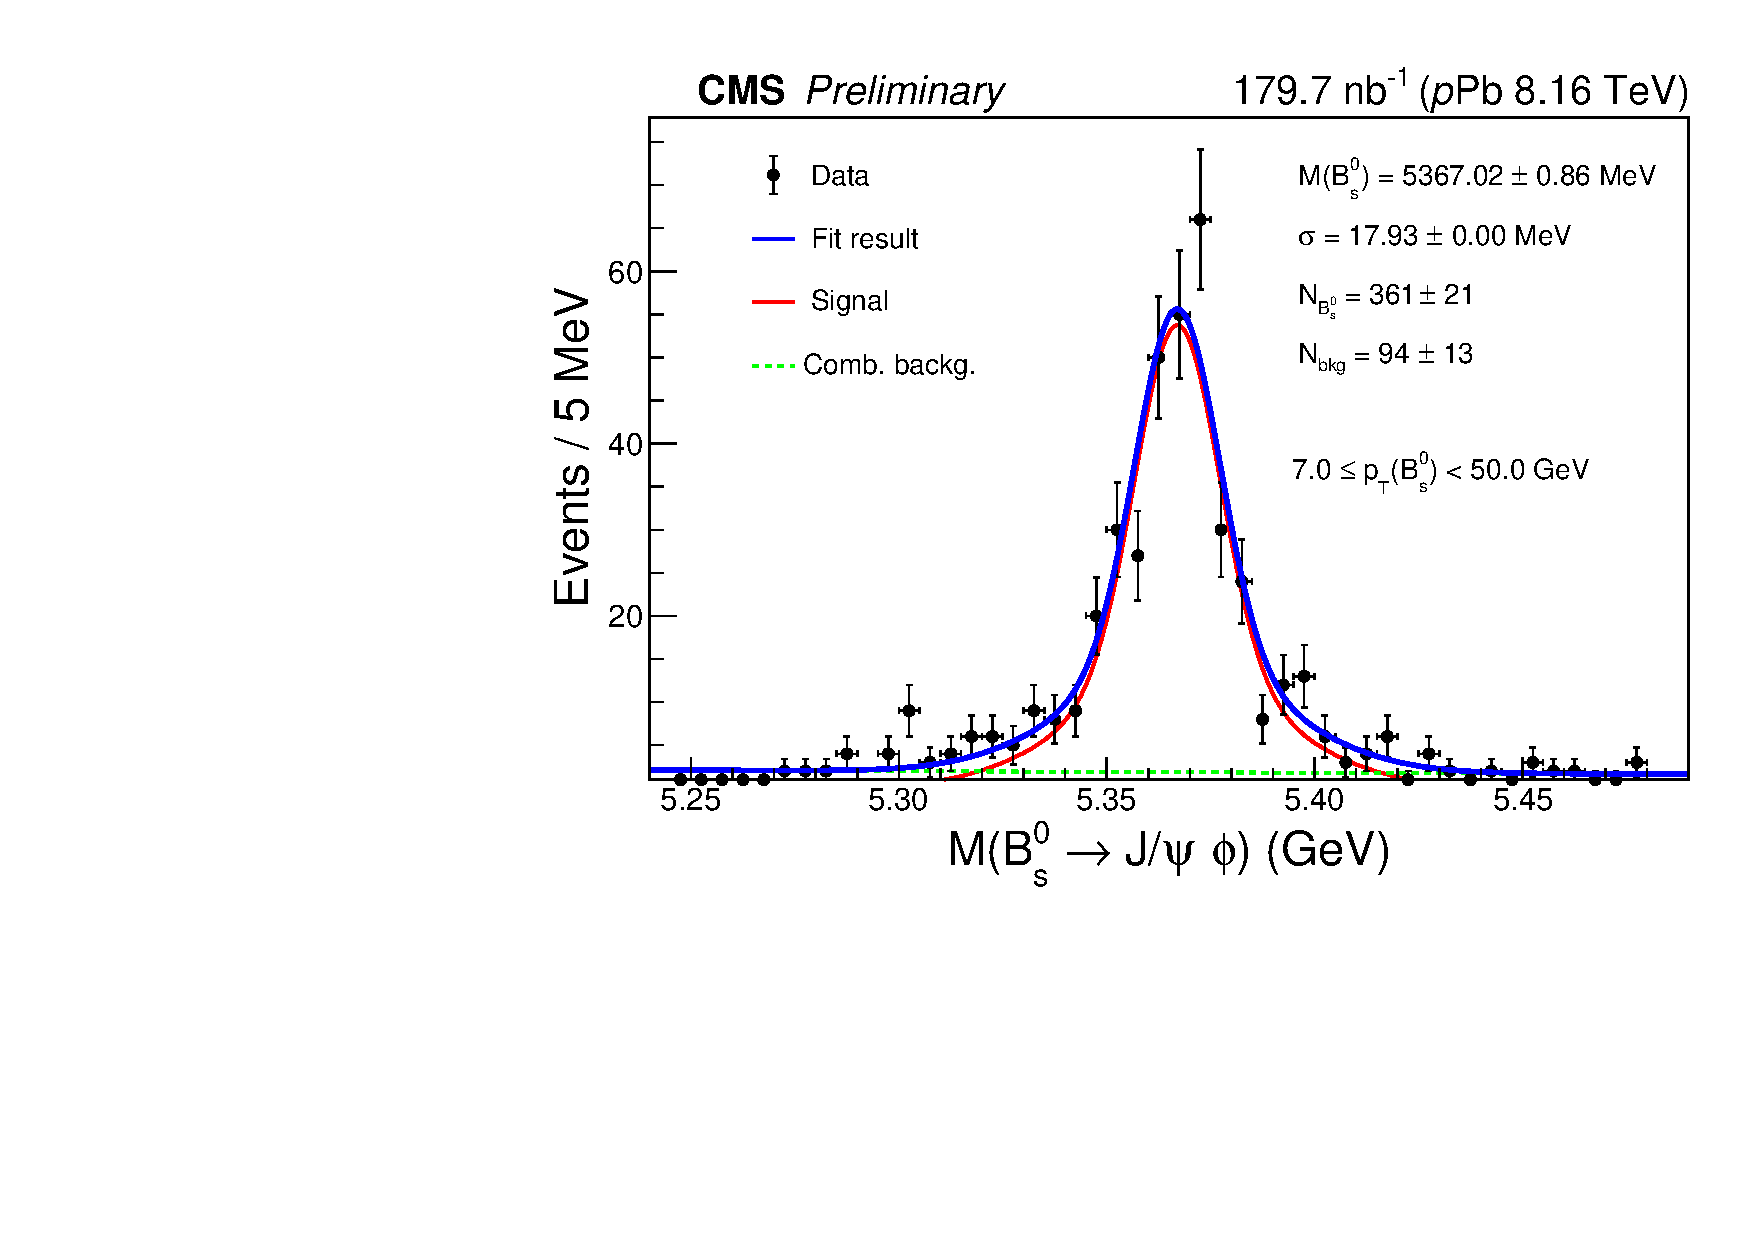
\includegraphics[width=\textwidth]{MainContent/Figs/mass/mass_BsFit_ptbins_7_50.PDF}}
		
	\end{subfigure}
	\caption{Invariant mass spectra for the $B^0_s$ meson using the data from p-Pb collision and considering the different bins for $p_T$. }
	%%%%%%%%%%%%%%%%%%%%%%%%%%%%%%%%%%%%second row
	
\end{figure}

\begin{figure}
	\centering
	\begin{subfigure}[t]{0.8\textwidth}
		\raisebox{-\height}{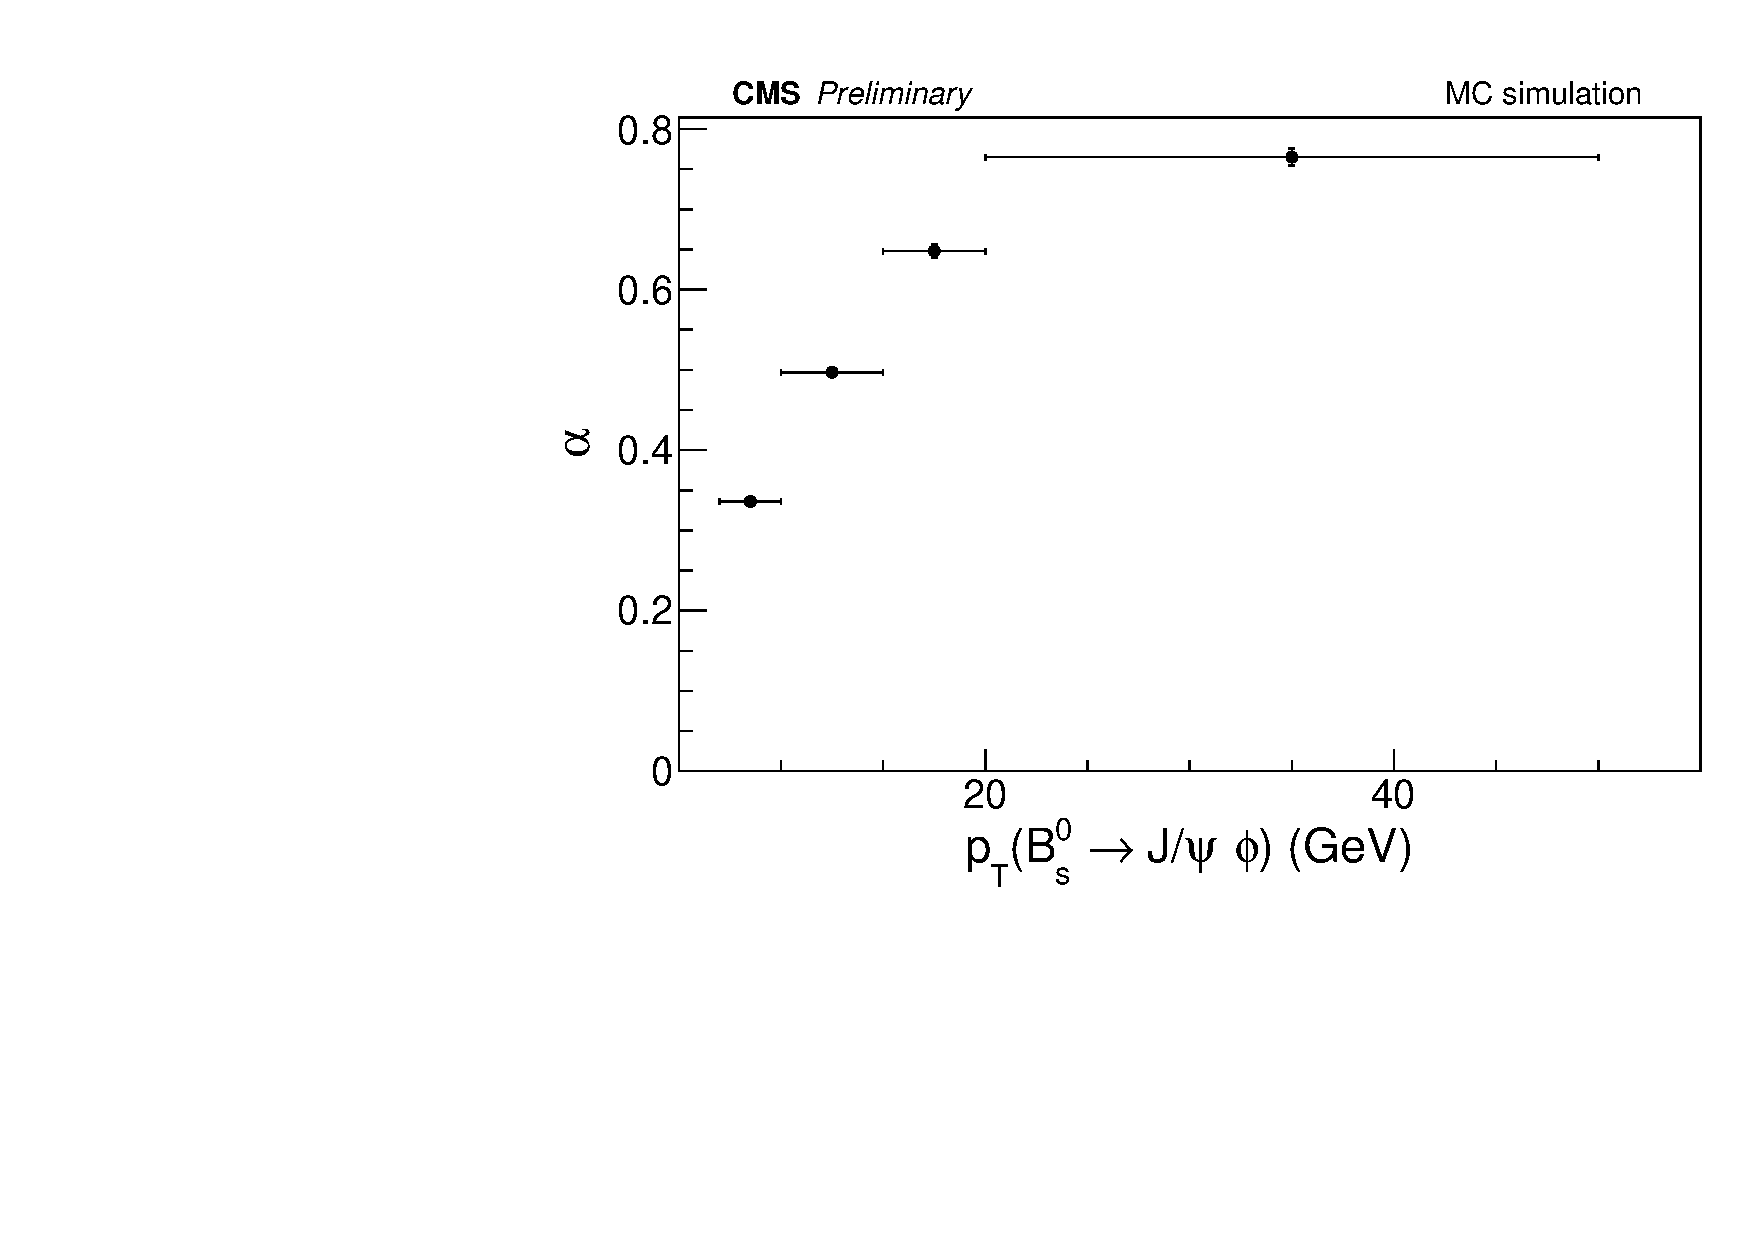
\includegraphics[width=0.49\textwidth]{MainContent/Figs/effy/Bseffy_prefilter.PDF}}
		\raisebox{-\height}{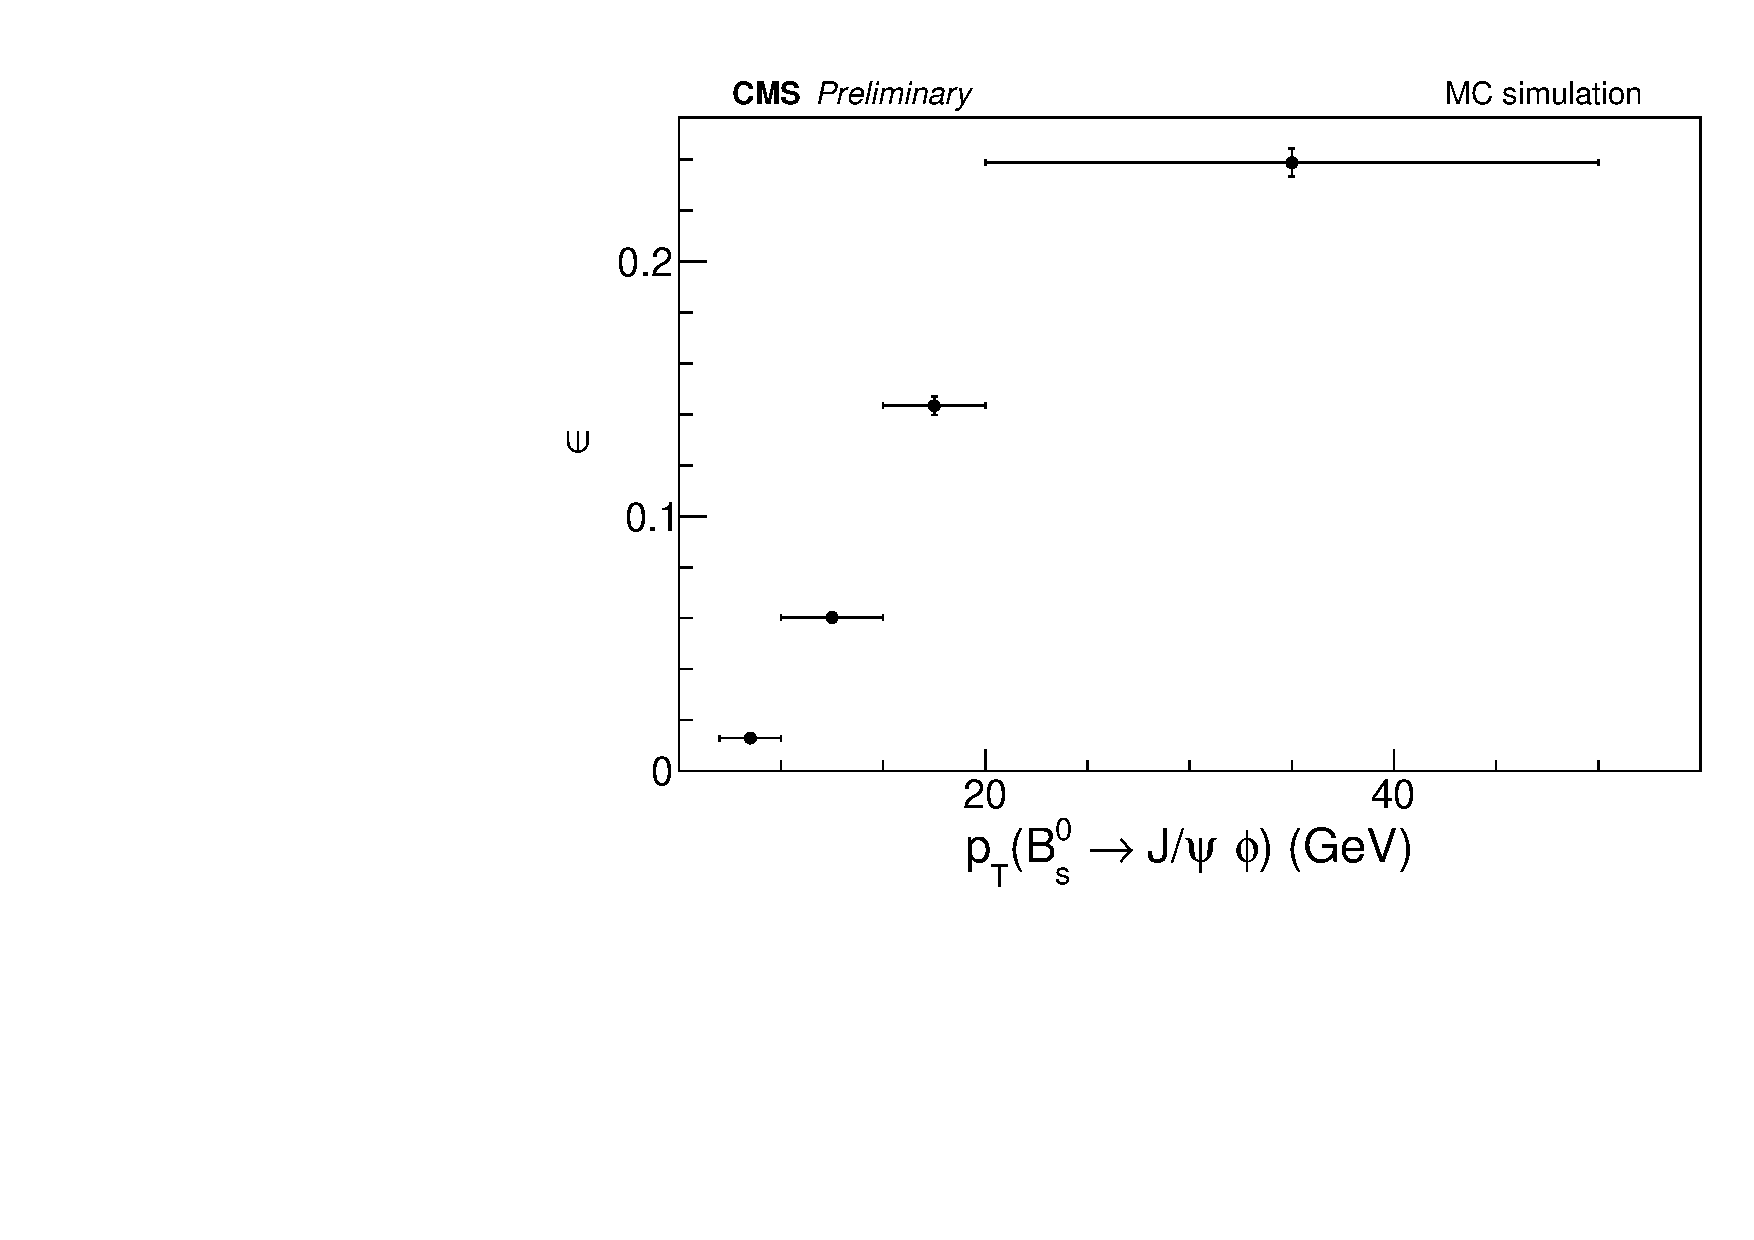
\includegraphics[width=0.49\textwidth]{MainContent/Figs/effy/Bseffy_reco.PDF}}%
	\end{subfigure}
	\hfill
	\begin{subfigure}[t]{0.8\textwidth}
		\raisebox{-\height}{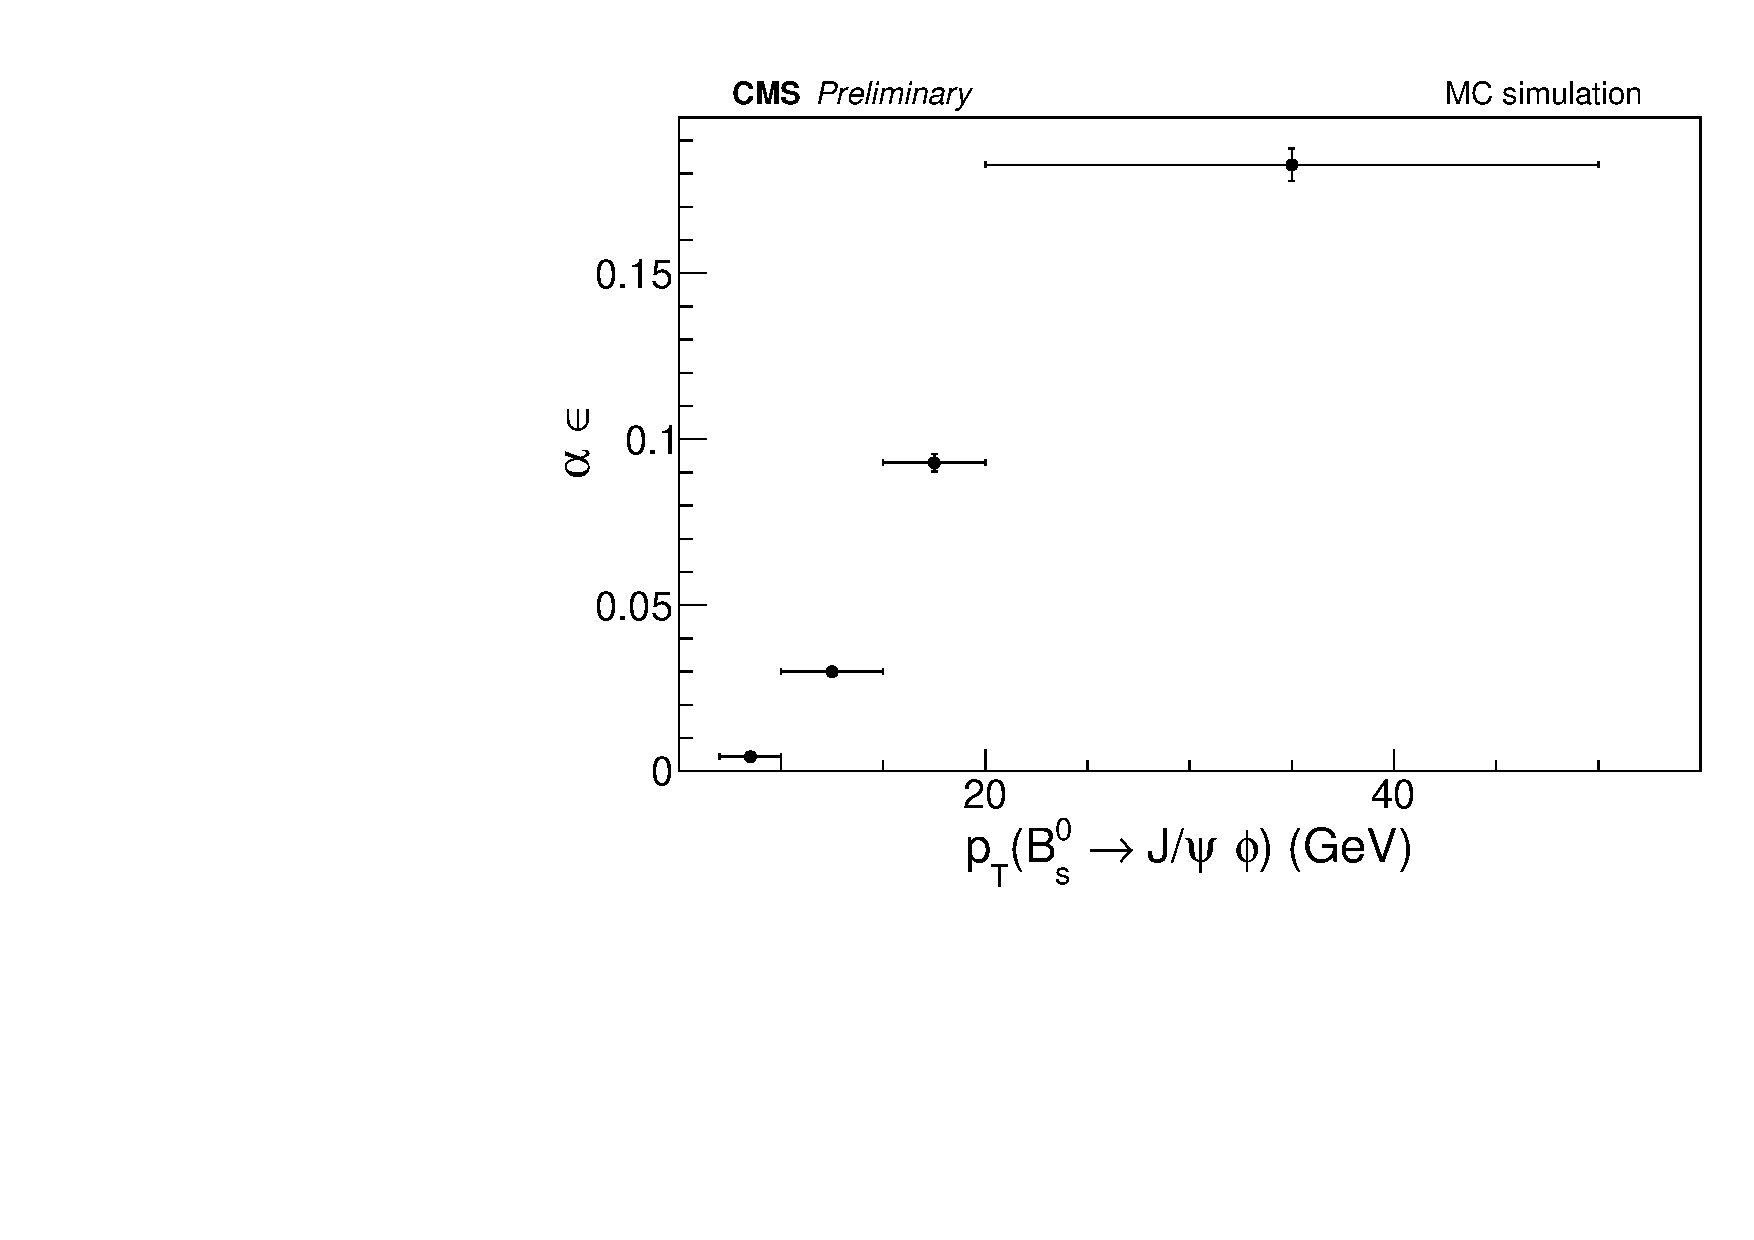
\includegraphics[width=\textwidth]{MainContent/Figs/effy/Bseffy_Total.PDF}}
		
	\end{subfigure}
	\caption{Acceptance, efficiency and total efficiency for the MC simulation.}
	%%%%%%%%%%%%%%%%%%%%%%%%%%%%%%%%%%%%second row
	
\end{figure}

\begin{figure}
	\centering
	\begin{subfigure}[t]{0.8\textwidth}
		\raisebox{-\height}{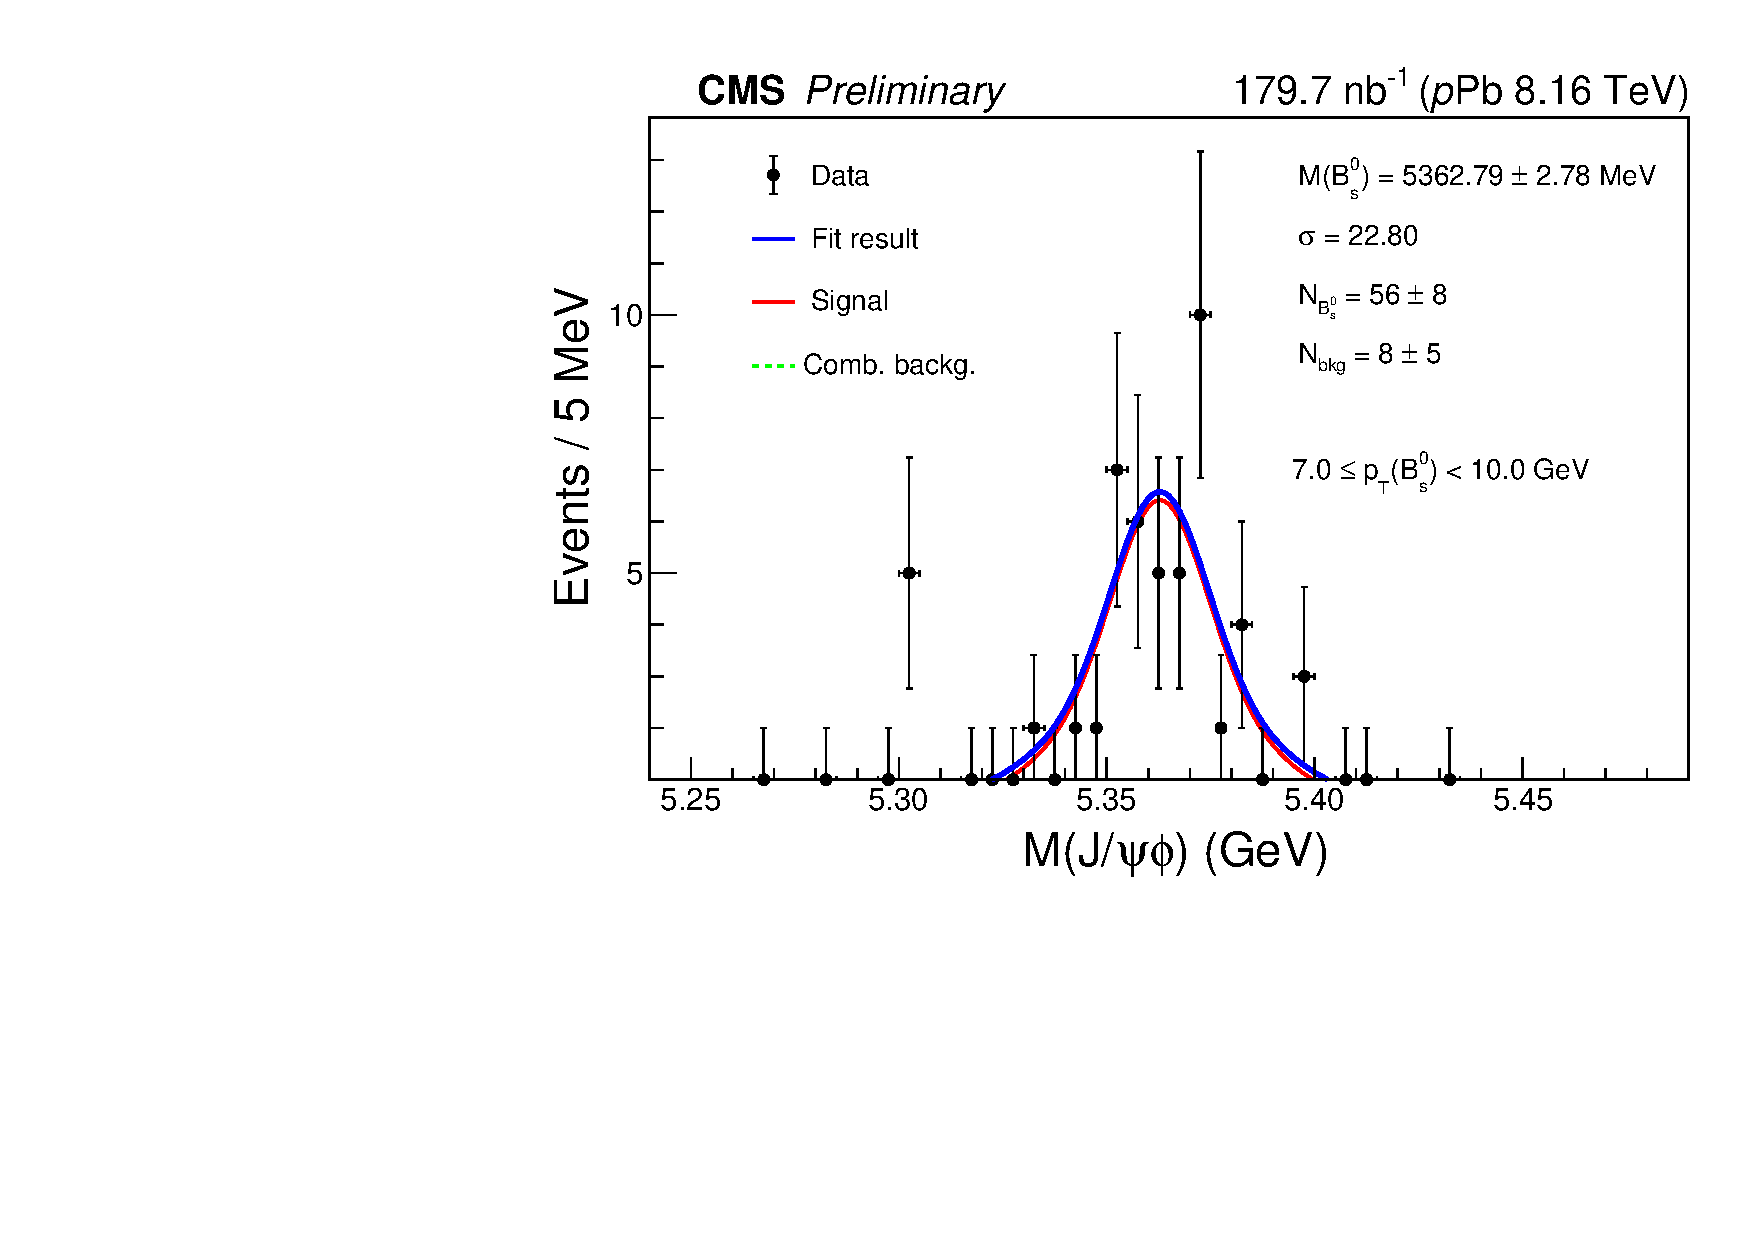
\includegraphics[width=0.49\textwidth]{MainContent/Figs/mass/mass_BsFit_ptbins_sysbkg_7_10.PDF}}
		\raisebox{-\height}{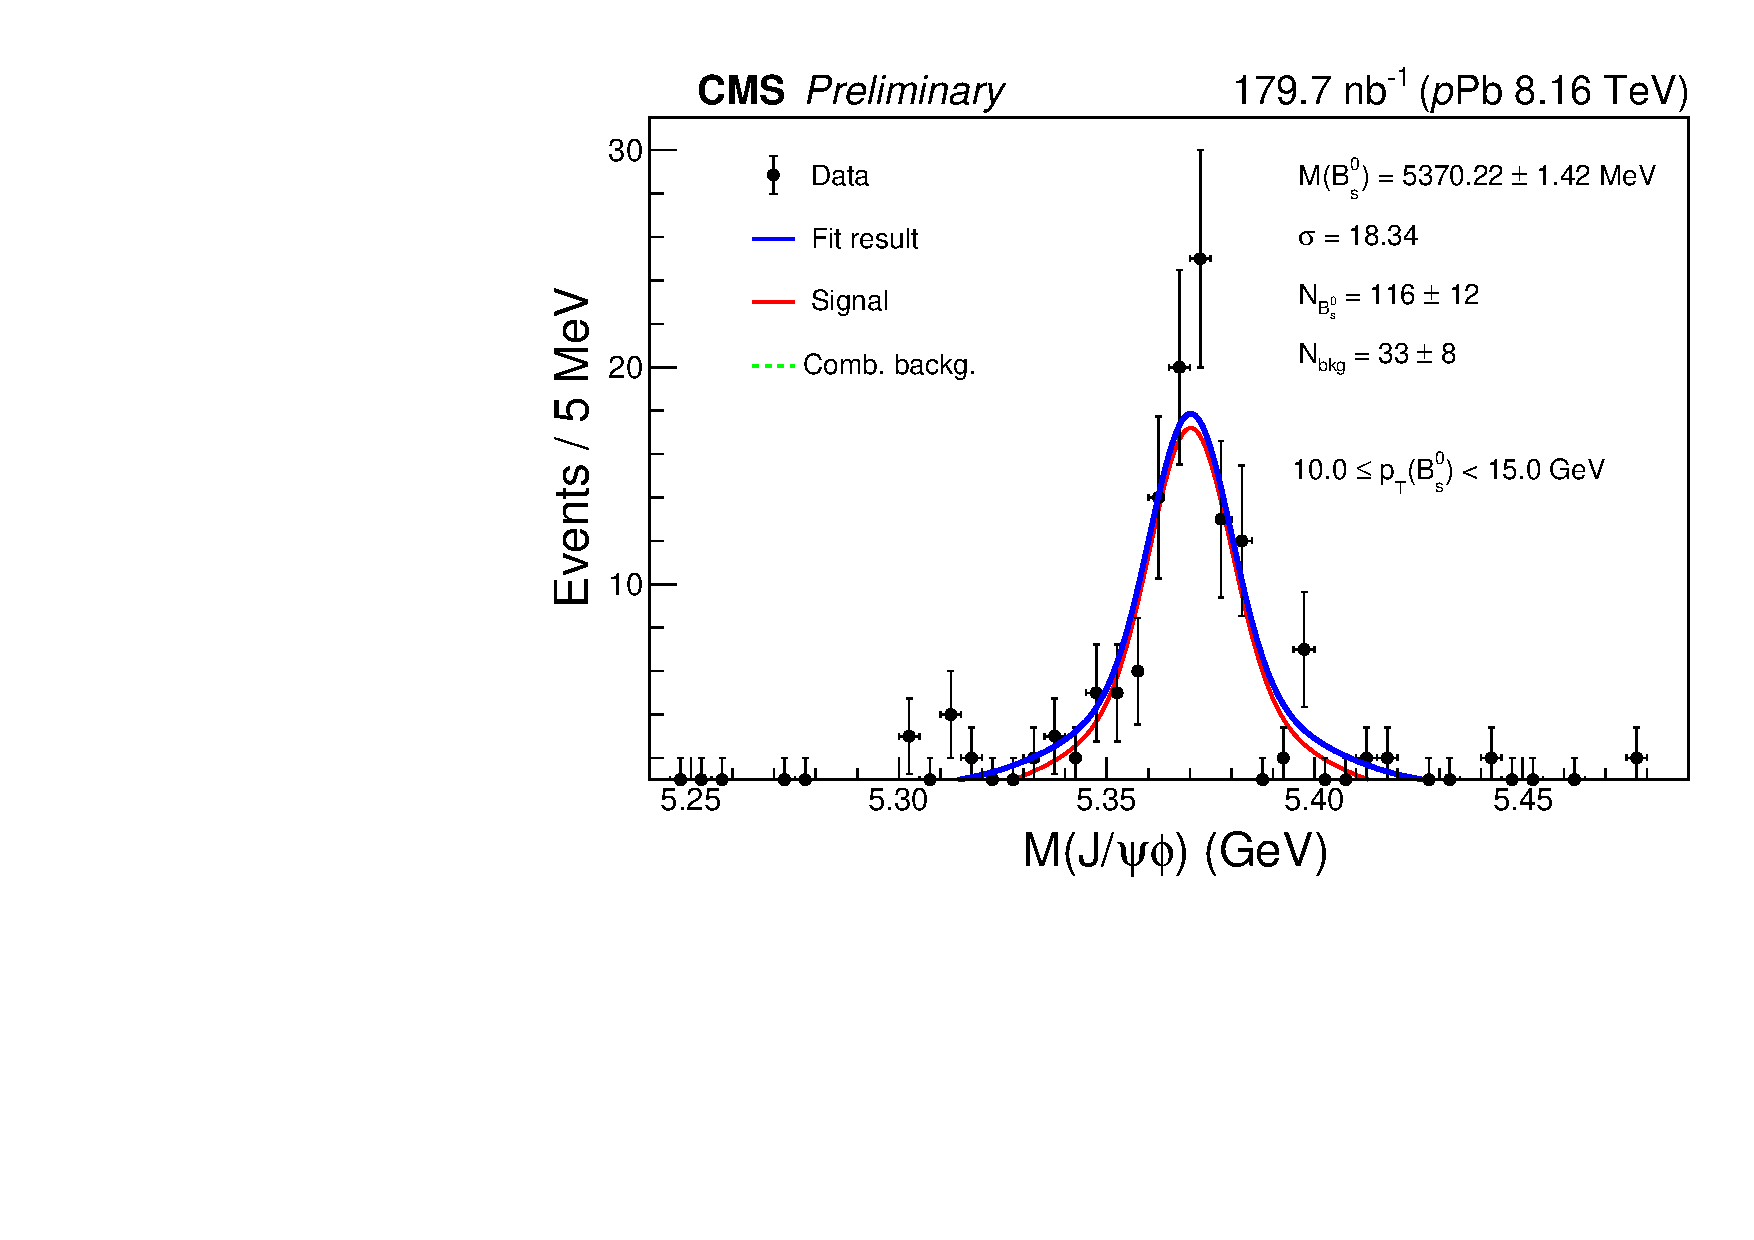
\includegraphics[width=0.49\textwidth]{MainContent/Figs/mass/mass_BsFit_ptbins_sysbkg_10_15.PDF}}%
		\vspace{.6ex}
		\raisebox{-\height}{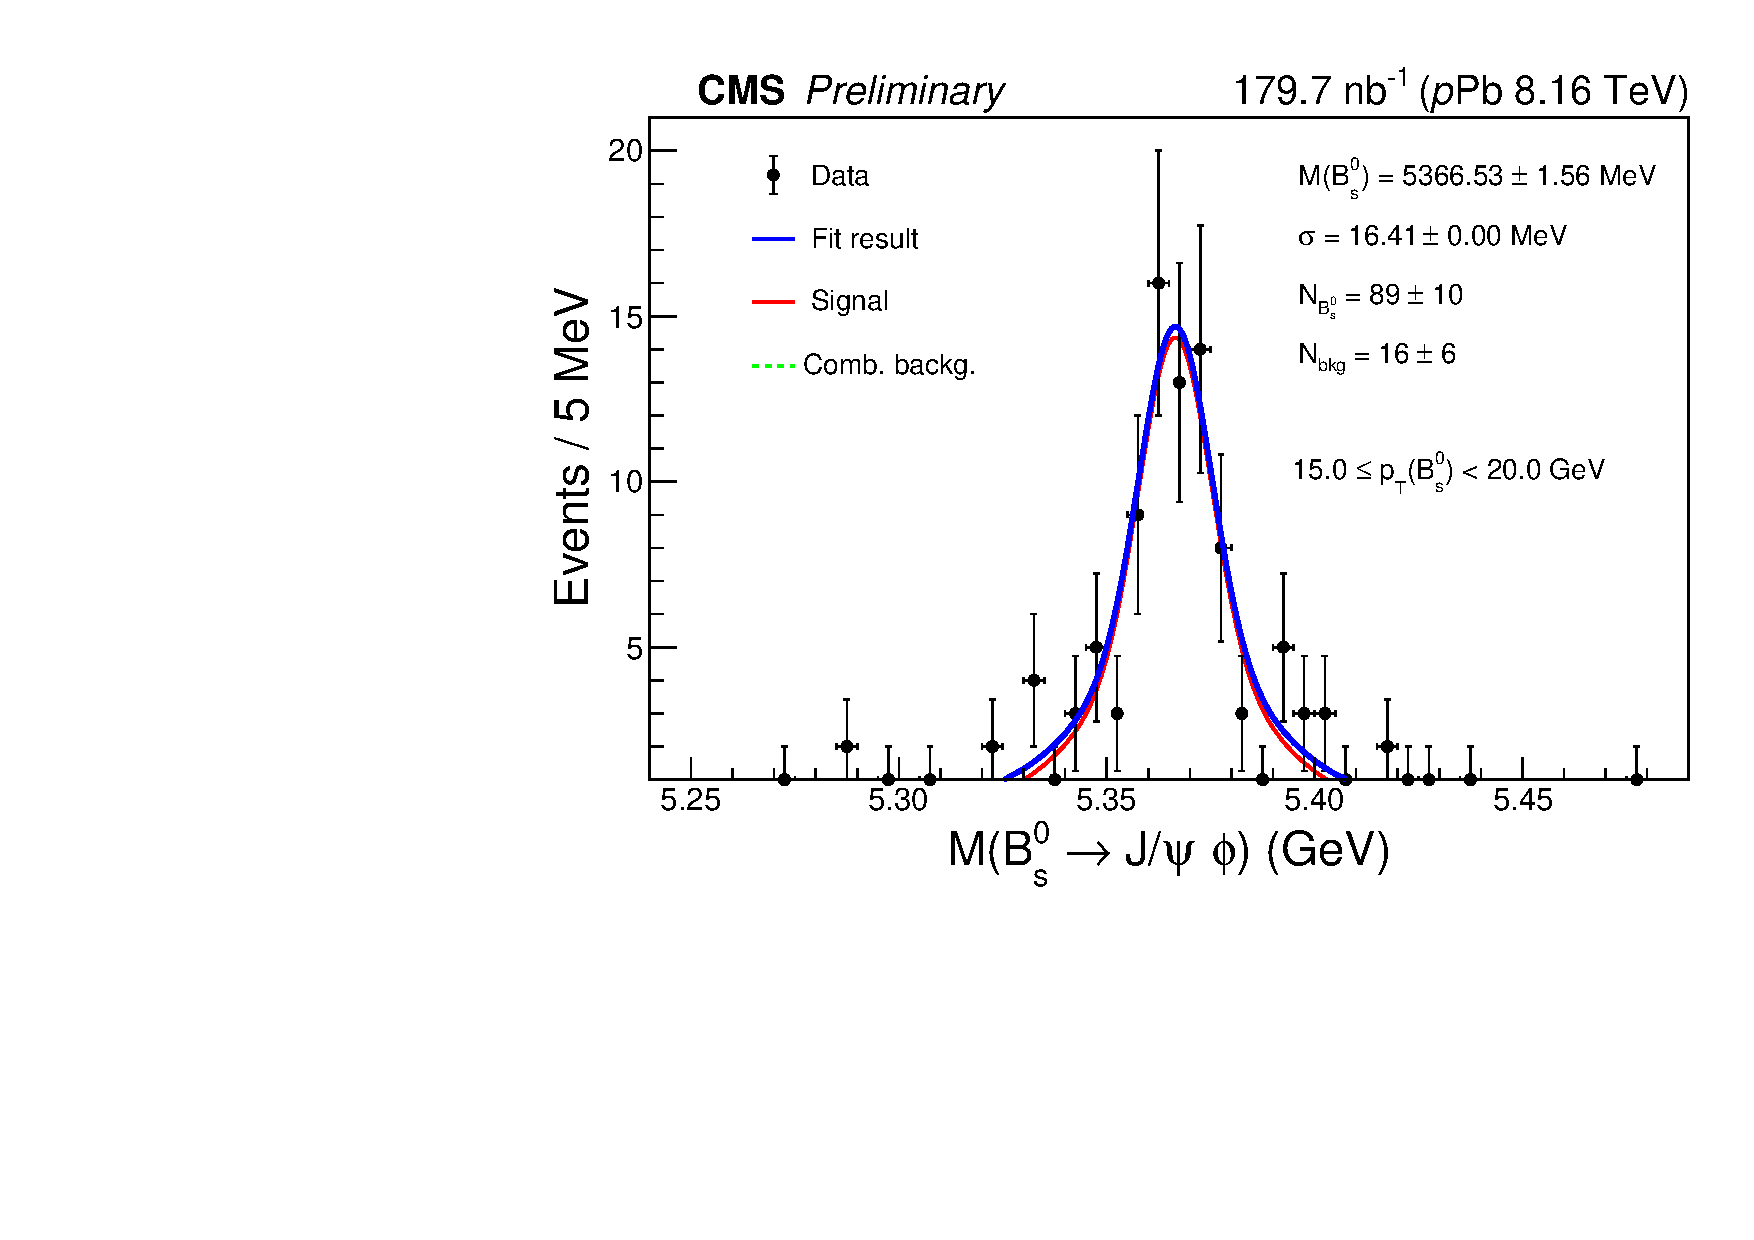
\includegraphics[width=0.49\textwidth]{MainContent/Figs/mass/mass_BsFit_ptbins_sysbkg_15_20.PDF}}
		\raisebox{-\height}{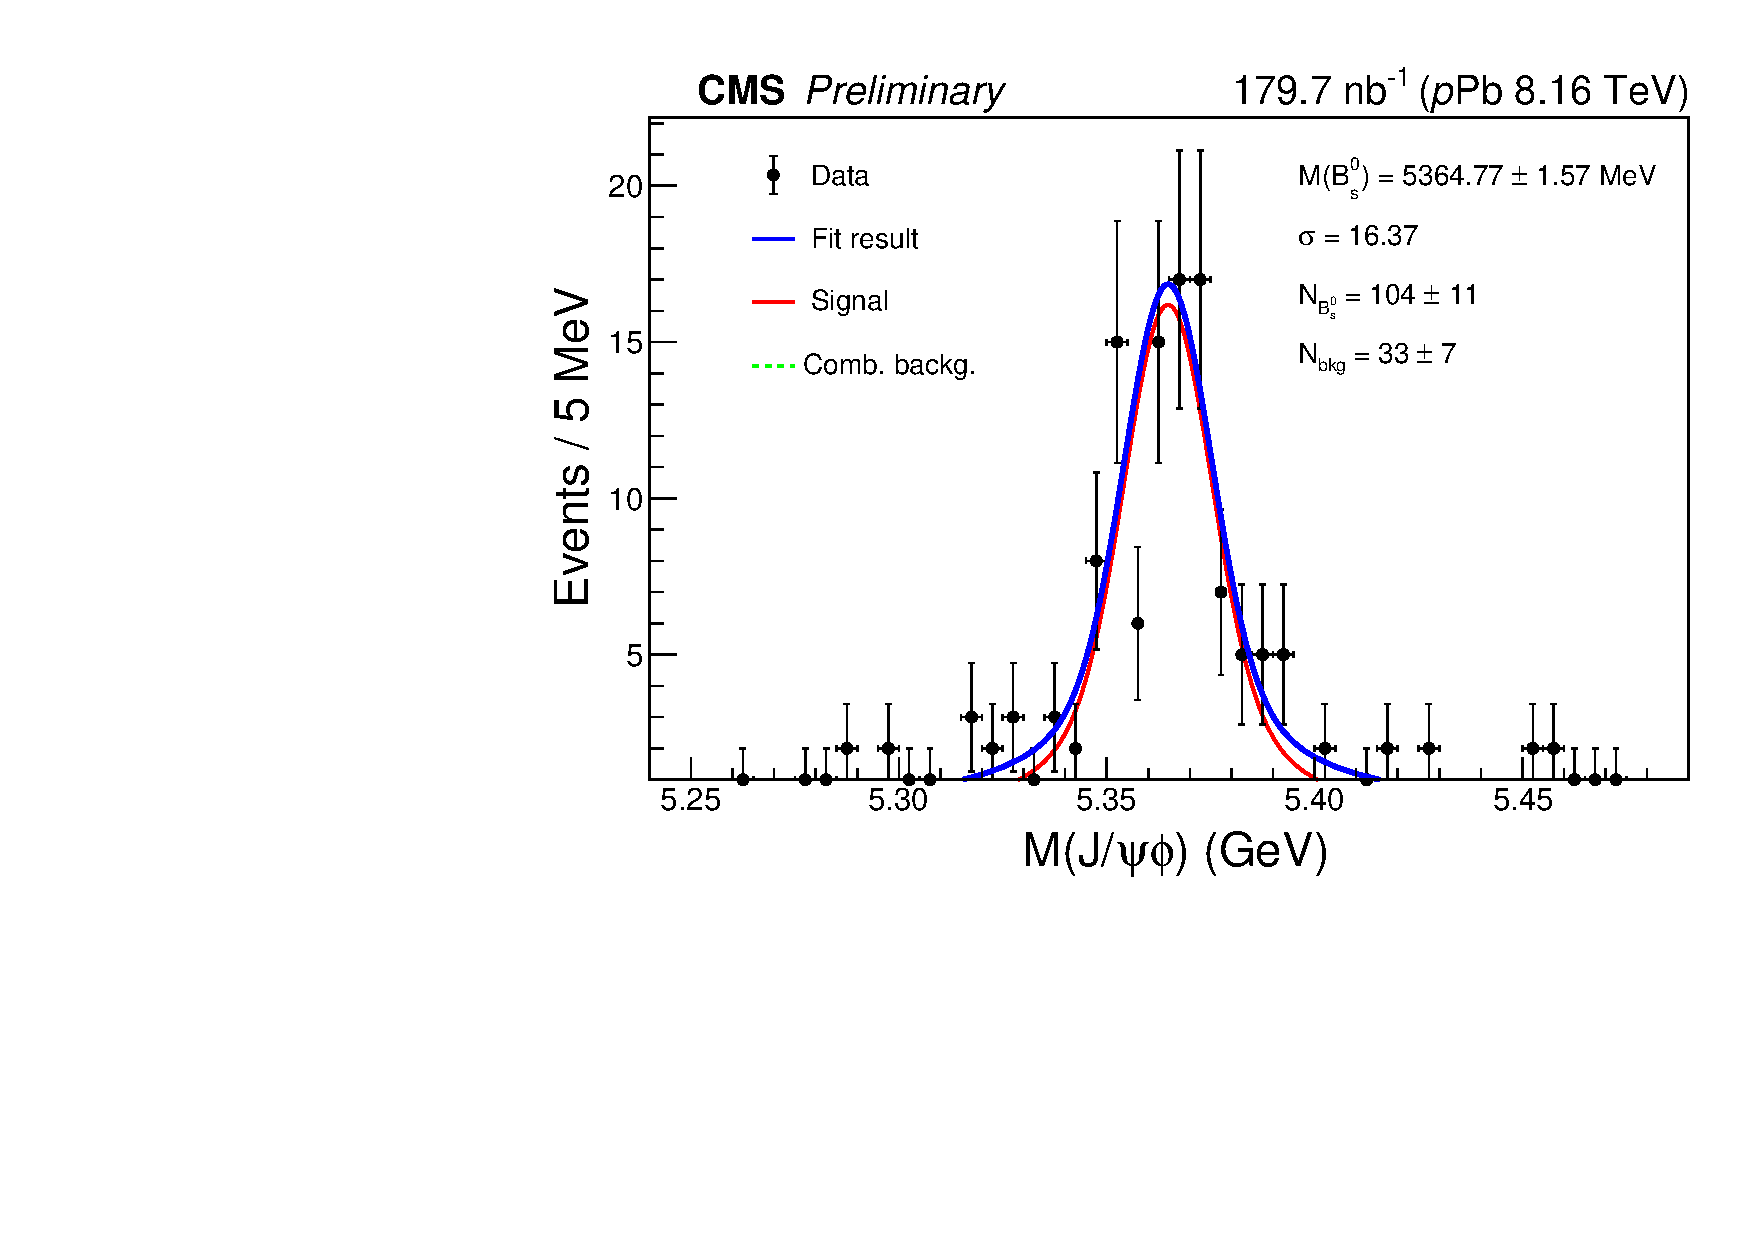
\includegraphics[width=0.49\textwidth]{MainContent/Figs/mass/mass_BsFit_ptbins_sysbkg_20_50.PDF}}%
	\end{subfigure}
	\hfill
	\begin{subfigure}[t]{0.8\textwidth}
		\raisebox{-\height}{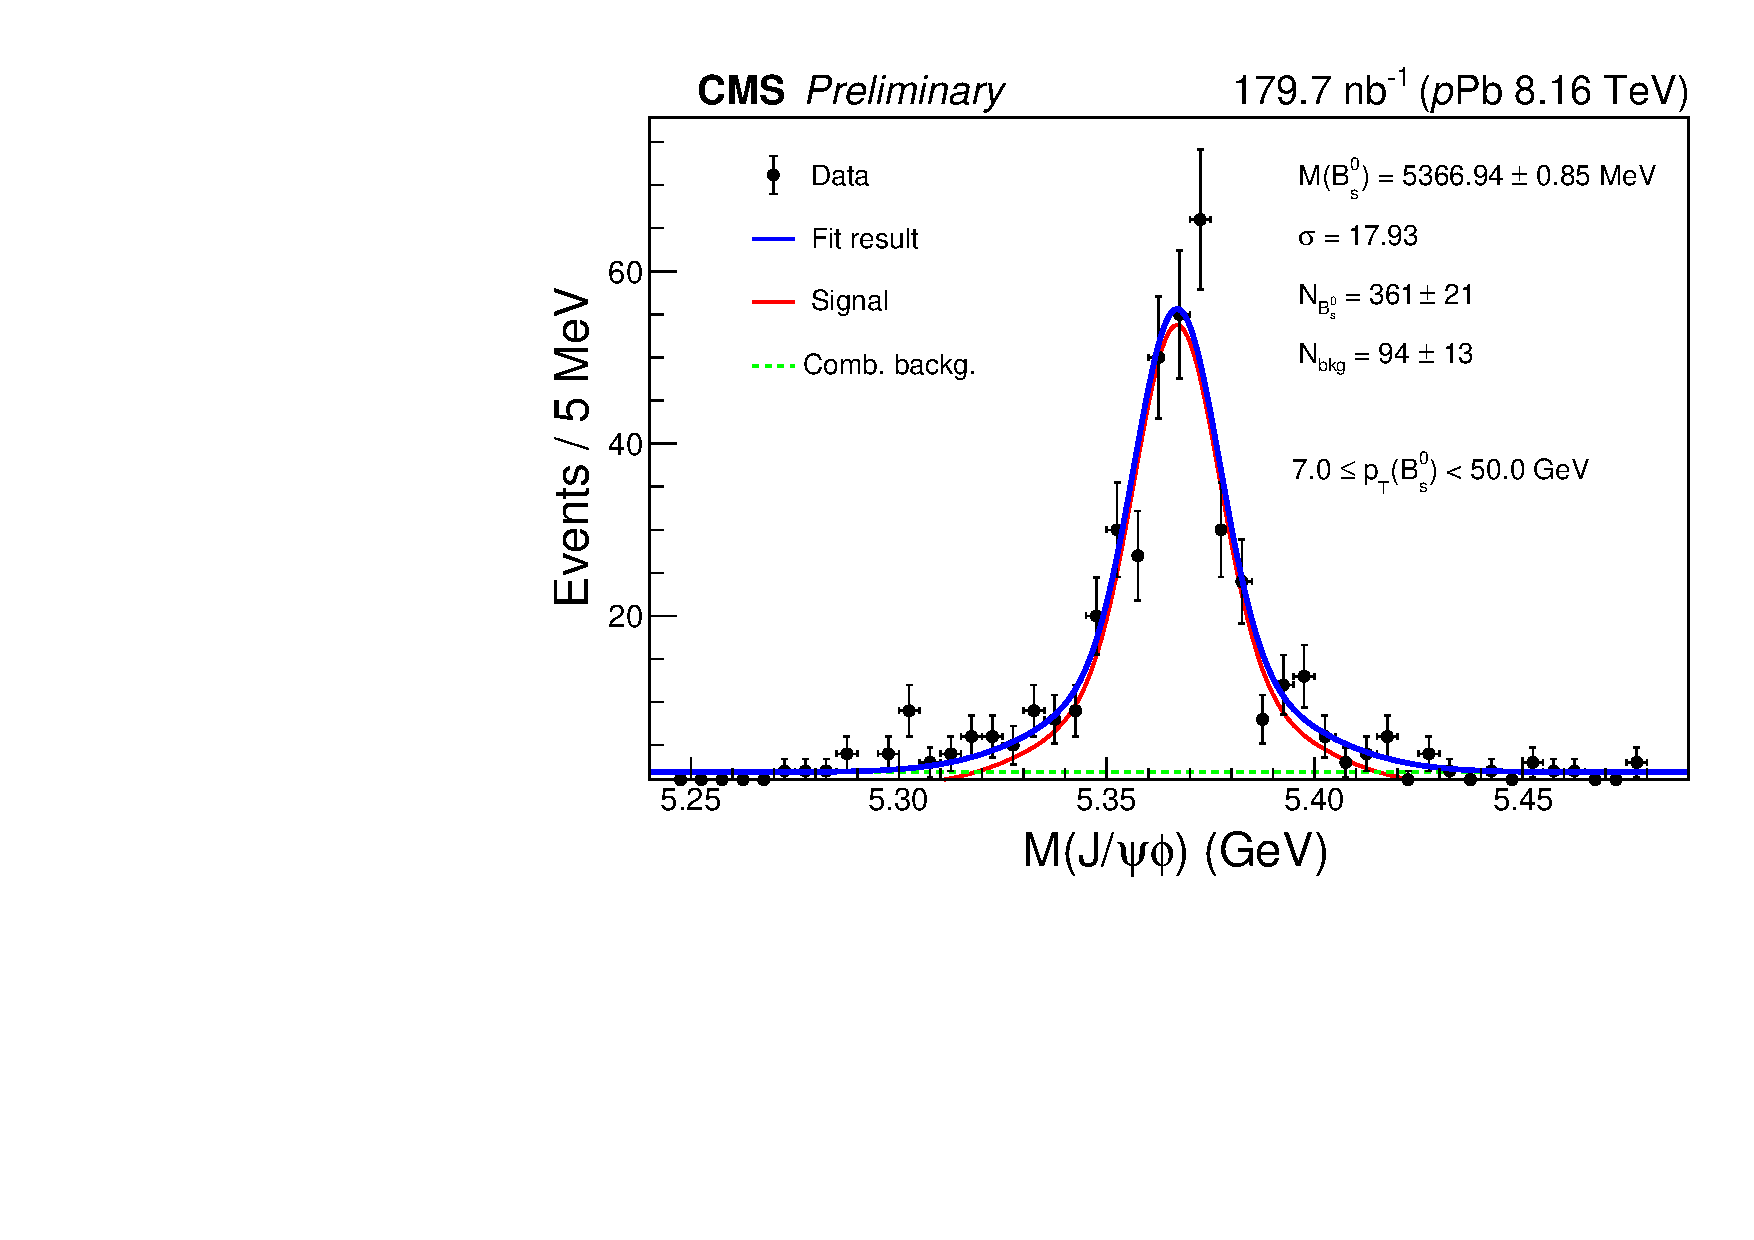
\includegraphics[width=\textwidth]{MainContent/Figs/mass/mass_BsFit_ptbins_sysbkg_7_50.PDF}}
		
	\end{subfigure}
	\caption{Invariant mass spectra for the $B^0_s$ meson using the data from p-Pb collision and a different model for the background data.}
	%%%%%%%%%%%%%%%%%%%%%%%%%%%%%%%%%%%%second row
	
\end{figure}

\begin{figure}
	\centering
	\begin{subfigure}[t]{0.8\textwidth}
		\raisebox{-\height}{\includegraphics[width=0.49\textwidth]{MainContent/Figs/mass/mass_BsFit_ptbins_syssig_7_10.PDF}}
		\raisebox{-\height}{\includegraphics[width=0.49\textwidth]{MainContent/Figs/mass/mass_BsFit_ptbins_syssig_10_15.PDF}}%
		\vspace{.6ex}
		\raisebox{-\height}{\includegraphics[width=0.49\textwidth]{MainContent/Figs/mass/mass_BsFit_ptbins_syssig_15_20.PDF}}
		\raisebox{-\height}{\includegraphics[width=0.49\textwidth]{MainContent/Figs/mass/mass_BsFit_ptbins_syssig_20_50.PDF}}%
	\end{subfigure}
	\hfill
	\begin{subfigure}[t]{0.8\textwidth}
		\raisebox{-\height}{\includegraphics[width=\textwidth]{MainContent/Figs/mass/mass_BsFit_ptbins_syssig_7_50.PDF}}
		
	\end{subfigure}
	\caption{Invariant mass spectra for the $B^0_s$ meson using the data from p-Pb collision and and a different model for the signal data.}
	%%%%%%%%%%%%%%%%%%%%%%%%%%%%%%%%%%%%second row
	
\end{figure}


\subsection{$|y|$ bins}

\section{Total efficiency}

\section{Systematic models}


\section{Differential cross-section}

% Chapter 7
\chapter{\leavevmode\newline  Conclusion}
\label{chap:conclusion}
Cheers!!!

\clearpage

% % Appendices
% \begin{appendices}

\addtocontents{toc}{\protect\renewcommand{\protect\cftchappresnum}{\appendixname\space}}
\addtocontents{toc}{\protect\renewcommand{\protect\cftchapnumwidth}{6em}}

\chapter{This is Appendix}
Add more chapters of appendices if need to.

\end{appendices}

% Reference
%========================================
\addcontentsline{toc}{chapter}{Bibliography}
\begin{singlespace}
	\setlength\bibitemsep{\baselineskip}
	\printbibliography[title={Bibliography}]
\end{singlespace}

\end{document}